\definecolor{celeste}{RGB}{166, 201, 236}
\definecolor{azul1}{RGB}{218, 233, 248}
\definecolor{azul2}{RGB}{192, 230, 245}
\definecolor{azul3}{RGB}{148, 220, 248}
\definecolor{azul4}{RGB}{97, 203, 243}
\definecolor{azul5}{RGB}{68, 179, 225}
\definecolor{azul6}{RGB}{100, 149, 237}
\definecolor{azul7}{RGB}{84, 127, 222}
\definecolor{azul8}{RGB}{77, 147, 217}
\definecolor{azul9}{RGB}{0, 134, 234}
\definecolor{azul10}{RGB}{0, 120, 210}

\chapter{Validación de sensor de distancia tipo láser}

En este capítulo se presentan las alternativas de sensores de distancia tipo láser consideradas y la validación de la selección del sensor más adecuado para la futura implementación de algoritmos de exploración y mapeo de entornos en agentes robóticos móviles. Cada uno de los sensores analizados presenta ventajas específicas, por lo que, con el fin de identificar aquel que mejor se adaptara a las necesidades de esta aplicación, se realizó un \textit{trade study} en el cual se evaluaron diversos parámetros y especificaciones de cada uno de estos. Este análisis comparativo asegura que la elección final ofrezca el mejor rendimiento posible según criterios relevantes para la aplicación.

\section{Sensores de distancia tipo láser considerados}
Las opciones de sensores de distancia tipo láser consideradas para este trabajo fueron: el módulo VL53L0X, el LiDAR FHL-LD20 y el YDLIDAR Tmini Pro. Estos sensores fueron seleccionados estratégicamente para analizar dos tecnologías de medición diferentes: triangulación y tiempo de vuelo (ToF, por sus siglas en inglés). Ambas tecnologías han demostrado ser altamente efectivas en la obtención de mediciones de distancia para aplicaciones de navegación autónoma, haciendo que los sensores que las utilizan sean candidatos adecuados para la aplicación prevista.

\subsection{Sensor VL53L0X}
El sensor de distancia láser VL530X de STMicroelectronics \cite{stmicroelectronics_vl53l0x_2016} es un módulo compacto con microcontrolador integrado que utiliza la tecnología de medición por tiempo de vuelo para obtener mediciones precisas, independientemente de la reflectancia del objetivo. Es capaz de medir distancias con precisión en un rango de 50 mm a 2 m. Una  característica destacada de este sensor es su emisor láser de cavidad vertical de 940 nm, el cual es completamente invisible para el ojo humano durante su funcionamiento. 
 
Con un campo de visión (FoV) típico de 25°, el sensor integra una avanzada matriz SPAD, capaz de detectar fotones individuales incluso en condiciones de luz extremadamente débil. Esta característica junto con sus filtros anti-infrarrojos, mejora significativamente la sensibilidad y precisión de las mediciones en entornos con niveles altos de luz infrarroja. Adicionalmente, su interfaz $I^2C$ estándar facilita el control y transferencia de datos, lo que simplifica su integración en proyectos electrónicos. Por estas razones, es ampliamente utilizado en aplicaciones como prevención de colisiones, detección de bordes, o en sistemas de auto-enfoque en cámaras digitales \cite{stmicroelectronics_vl53l0x_2016}.

\subsection{LiDAR FHL-LD20}

El LiDAR FHL-LD20, desarrollado por youyeetoo Tech \cite{youyeetoo_tech_ld20_nodate}, es un sensor omnidireccional de 360° que emplea tecnología de triangulación para escanear su entorno. Una vez recopilados los datos de distancia, el sensor combina estos valores con los ángulos medidos por la unidad de medición angular para generar una nube de puntos, que puede utilizarse para crear un mapa detallado del contorno circundante. Además, cuenta con un CCD fotosensible de alto rendimiento, el cual le permite medir distancias con precisión en un rango de 100 mm a 8 m. 

El núcleo de medición de distancia del FHL-LD20 permite capturar 4000 puntos por segundos, lo que facilita la actualización del entorno capturado. Esta capacidad, junto con la modulación de la velocidad del motor, mejora la cobertura del sensor y reduce los puntos ciegos en distintos entornos. Adicionalmente, su comunicación serial UART simplifica la integración del LiDAR en una amplia variedad de aplicaciones, como la navegación autónoma en robots móviles, la reconstrucción de mapas 2D y la elusión de obstáculos \cite{youyeetoo_tech_ld20_nodate}.

\subsection{YDLIDAR Tmini Pro}

El YDLIDAR Tmini Pro es un LiDAR 2D de 360° desarrollado por EAI Technology \cite{eai_technology_ydlidar_2022}. Emplea el principio de tiempo de vuelo para lograr mediciones de distancia con alta precisión. Durante la medición, su estructura mecánica gira 360 grados, lo que le permite obtener información continua de ángulos y realizar un escaneo completo del entorno. Entre sus características destacadas se encuentra su resistencia al polvo y al agua, lo que lo hace adecuado para operar en condiciones ambientales adversas.

Junto a esto, su tamaño compacto facilita su integración a otros sistemas, optimizando la estructura espacial en una amplia variedad de aplicaciones. Esto lo hace adecuado para pruebas en diversos escenarios. Utiliza comunicación serial UART para transmitir los datos de medición, lo que simplifica su conexión con sistemas de procesamiento. Con un rango de medición de 20 mm a 12 m, el YDLIDAR Tmini Pro es empleado en navegación y elusión de obstáculos en robots de servicio doméstico y aspiradoras robot, mejorando su eficiencia y capacidad de respuesta en entornos complejos \cite{eai_technology_ydlidar_2022}.

\section{Selección del sensor de distancia tipo láser}
Los sensores descritos en la sección anterior fueron evaluados considerando sus diferencias en metodología de medición y cantidad de datos generados. Aunque los tres sensores comparten el mismo propósito, estas variaciones presentan ventajas y desventajas específicas en función del objetivo y contexto de cada proyecto. Por esta razón, para realizar una comparación efectiva entre estos, se establecieron distintos criterios que se consideraron fundamentales para el desarrollo de este trabajo.

En el Cuadro \ref{cuadro:criterios} se presentan los criterios empleados en el \textit{trade study} junto con el peso asignado a cada parámetro. Estos pesos fueron determinados mediante el proceso de ponderación por pares, un método utilizado para comparar y sopesar criterios cualitativos y cuantitativos entre sí. Para este estudio, se consideraron 10 criterios para asegurar una decisión fundamentada al escoger el sensor.

\begin{table}[H]
	\centering
	\begin{tabular}{|l|r|}
		\hline
		\multicolumn{1}{|c|}{\textbf{Criterios}}&\multicolumn{1}{|c|}{\textbf{Peso}}\\ 
		\hline
		Costo&$10\%$\\
		\hline
		Disponibilidad&$15\%$\\
		\hline
		Precisión&$6\%$\\
		\hline
		Rango de medición&$7\%$\\
		\hline
		Parámetros eléctricos&$5\%$\\
		\hline
		Velocidad de medición&$6\%$\\
		\hline
		Tamaño&$6\%$\\
		\hline
		Masa&$8\%$\\
		\hline
		Operatividad en aplicaciones deseadas&$22\%$\\
		\hline
		Adaptabilidad a robots móviles&$15\%$\\
		\hline
	\end{tabular}
	\caption{Criterios de comparación.} 
	\label{cuadro:criterios}
\end{table}

El método de ponderación por pares emplea una matriz de comparaciones (ver Cuadro \ref{cuadro:matrizPP}) para evaluar la importancia relativa entre cada par de criterios. Primero, se calcula la media geométrica de los valores en cada fila de la matriz. Luego, estos valores se normalizan para obtener los factores de ponderación, garantizando que la suma total sea igual a 1 \cite{fatchurrahman_light_2016}. Los valores para las comparaciones se seleccionan dentro de un intervalo 1 a 9, como se describe en el Cuadro \ref{cuadro:valoresPP}.

\begin{table}[H]
	\centering
	\rotatebox{90}{
		\resizebox{0.98\textheight}{!}{
			\begin{tabular}{|c|c|c|c|c|c|c|c|c|c|c|c|c|}
				\hline
				&Costo&Disponibilidad&Precisión&\makecell{Rango\\de medición}&\makecell{Parámetros\\eléctricos}&\makecell{Velocidad\\de medición}&Tamaño&Peso&Operatividad&Adaptabilidad&\makecell{Media\\ Geométrica}&Masa\\
				\hline
				Costo&1&1/4&1/2&3&2&5&4&4&1/5&1/3&1.1487&0.1019
				\\
				\hline
				Disponibilidad&4&1&3&2&2&4&3&3&1/3&1/4&1.6438&0.1458
				\\
				Precisión&2&1/3&1&7&3&1&1/4&1/4&1/8&1/6&0.6700&0.0594
				\\
				\hline
				\makecell{Rango\\de medición}&1/3&1/2&1/7&1&5&1/3&5&5&1/3&1/4&0.7794&0.0691
				\\
				\hline
				\makecell{Parámetros\\eléctricos}&1/2&1/2&1/3&1/5&1&1/5&2&1/2&1/2&3&0.5887&0.0522
				\\
				\hline
				\makecell{Velocidad\\de medición}&1/5&1/4&1&3&5&1&1/4&1/4&1&1/2&0.6871&0.0609
				\\
				\hline
				Tamaño&1/4&1/3&4&1/5&1/2&4&1&1&1/5&1&0.6960&0.0617
				\\
				\hline
				Masa&1/4&1/3&4&1/5&2&4&1&1&1/3&1&0.8414&0.0746
				\\
				\hline
				Operatividad&5&3&8&3&2&1&5&3&1&1&2.5313&0.2244
				\\
				\hline
				Adaptabilidad&3&4&6&4&1/3&2&1&1&1&1&1.6917&0.1500
				\\
				\hline
				\multicolumn{11}{|r|}{Suma}&11.2779&1.0000
				\\
				\hline
			\end{tabular}
		}
	}
	\caption{Matriz de comparación por pares.} 
	\label{cuadro:matrizPP}
\end{table}

\begin{table}[H]
	\centering
	\begin{tabular}{|c|l|}
		\hline
		\multicolumn{1}{|c|}{\textbf{Valor}}&\multicolumn{1}{|c|}{\textbf{Descripción}}\\ \hline
		1&Igual importancia\\ \hline
		3&Moderadamente más importante\\ \hline
		5&Fuertemente más importante\\ \hline
		7&Muy fuertemente más importante\\ \hline
		9&Extremadamente más importante\\ \hline
		2,4,6,8&Valores intermedios entre los anteriores\\ \hline
		
	\end{tabular}
	\caption{Escala fundamental de comparación por pares.} 
	\label{cuadro:valoresPP}
\end{table}

\subsection{Criterios para el \textit{Trade Study} de los sensores de distancia tipo láser}
El \textit{trade study} es un método sistemático de toma de decisiones diseñado para identificar la solución técnica más adecuada entre un conjunto de alternativas viables. Este enfoque consiste en evaluar y comparar diferentes opciones en función de una serie de criterios predefinidos, los cuales son ponderados numéricamente según su importancia relativa en el proyecto. A cada criterio se le asigna un peso específico, de manera que las alternativas que satisfacen más plenamente con dicho criterio obtengan una puntuación superior a aquellas que lo satisfacen en menor medida. El Cuadro \ref{cuadro:valoresCompa} muestra las calificaciones posibles al desempeño de cada uno de los criterios evaluados.

\begin{table}[H]
	\centering
	\begin{tabular}{|l|l|}
		\hline
		\multicolumn{1}{|c|}{\textbf{Adjetivos(s)}}&\multicolumn{1}{|c|}{\textbf{Calificación}}\\ \hline
		No aceptable / Nulo&0\\ \hline
		Muy malo / Muy bajo&1\\ \hline
		Malo / Bajo&2\\ \hline
		Moderado / Normal&3\\ \hline
		Bueno / Alto&4\\ \hline
		Muy bueno / Muy Alto&5\\ \hline
		
	\end{tabular}
	\caption{Valores de interés para la comparación.} 
	\label{cuadro:valoresCompa}
\end{table}

\subsubsection{Costo}
Dado que no se contaba con los dispositivos, fue necesario evaluar su compra. Para este criterio, se asignó la ponderación más alta al módulo VL53L0X, cuyo precio aproximo de \$6.00 lo hace más accesible que los otros sensores de distancia. Su precio resulta ser más de diez veces inferior al de los LiDAR evaluados. Cabe señalar que las ponderaciones asignadas a cada sensor en el Cuadro \ref{cuadro:ponderacionCosto} reflejan las limitaciones económicas del proyecto, donde se priorizaron las opciones que se ajustaran al presupuesto disponible. En el Cuadro \ref{cuadro:caracteristicasgenerales} se especifican los precios de los LiDAR, junto con características destacables que serán mencionadas en los criterios de evaluación.

\begin{table}[H]
	\centering
	\begin{tabular}{|l|l|}
		\hline
		\textbf{Alternativa} & \textbf{Costo} \\ \hline
		VL53L0X & 5 \\ \hline
		FHL-LD20 & 3 \\ \hline
		YDLIDAR Tmini Pro & 1 \\ \hline
	\end{tabular}
	\caption{Ponderación de costo.} 
	\label{cuadro:ponderacionCosto}
\end{table}


\subsubsection{Disponibilidad}
Este criterio es considerado uno de los más importantes, ya que la disponibilidad de un sensor influye directamente en diversos aspectos. Por un lado, un sensor que se encuentra ampliamente disponible permite realizar sustituciones rápidas y oportunas cuando sea necesario. Junto a esto, los sensores con amplia disponibilidad suelen ofrecer un mejor soporte técnico, lo que facilita su mantenimiento y desarrollo. En este contexto, como se muestra en el Cuadro \ref{cuadro:ponderacionDisponibilidad}, el módulo VL53L0X recibió la ponderación más alta, ya que es accesible en el mercado local de Guatemala. Es importante señalar que, aunque los otros dos sensores son desarrollados en el extranjero y generan un cargo adicional por envío, también cuentan con un excelente soporte técnico. 

\begin{table}[H]
	\centering
	\begin{tabular}{|l|l|}
		\hline
		\multicolumn{1}{|c|}{\textbf{Alternativas}}&\multicolumn{1}{|c|}{\textbf{Disponibilidad}}\\ \hline
		VL53L0X&5\\ \hline
		FHL-LD20&3\\ \hline
		YDLIDAR Tmini Pro&1\\ \hline
	\end{tabular}
	\caption{Ponderación de disponibilidad.} 
	\label{cuadro:ponderacionDisponibilidad}
\end{table}

\subsubsection{Precisión}
Como se indica en el Cuadro \ref{cuadro:caracteristicasgenerales}, la precisión de cada sensor se presenta dentro de un rango, donde el primer valor refleja la precisión en condiciones óptimas y el segundo corresponde a escenarios menos favorables. Aunque estos valores pueden fluctuar según el entorno donde se utilicen, los rangos proporcionan una idea general de la precisión de cada sensor. En este contexto, se observa que ambos sensores de distancia tipo láser LiDAR tienen una precisión inferior en comparación con el módulo VL53L0X. En particular, el FHL-LD20 muestra la menor precisión entre los tres sensores evaluados, lo que justifica su puntuación en el Cuadro \ref{cuadro:ponderacionPrecision}. 

\begin{table}[H]
	\centering
	\begin{tabular}{|l|l|}
		\hline
		\multicolumn{1}{|c|}{\textbf{Alternativas}}&\multicolumn{1}{|c|}{\textbf{Precisión}}\\ \hline
		VL53L0X&5\\ \hline
		FHL-LD20&3\\ \hline
		YDLIDAR Tmini Pro&4\\ \hline
	\end{tabular}
	\caption{Ponderación de precisión.} 
	\label{cuadro:ponderacionPrecision}
\end{table}

\subsubsection{Rango de medición}
El rango de medición del sensor debe ser adecuado para cubrir las dimensiones del área de trabajo. Puesto que se planea operar en el ecosistema Robotat, que cuenta con una plataforma de 4.8$\times$3.8 m, es importante que el sensor tenga un rango suficiente para medir distancias dentro de este espacio sin restricciones. Además, al considerar su futura integración con robots móviles para el mapeo de entornos, un rango de medición limitado podría restringir significativamente su utilidad. En este contexto, el FHL-LD20 obtiene la ponderación más alta (ver Cuadro \ref{cuadro:ponderacionRango}), ya que tiene la capacidad de cubrir áreas de trabajo moderadamente grandes como la plataforma del Robotat . 

\begin{table}[H]
	\centering
	\begin{tabular}{|l|l|}
		\hline
		\multicolumn{1}{|c|}{\textbf{Alternativas}}&\textbf{\makecell{Rango\\de medición}}\\ \hline
		VL53L0X&2\\ \hline
		FHL-LD20&5\\ \hline
		YDLIDAR Tmini Pro&4\\ \hline
		
	\end{tabular}
	\caption{Ponderación de rango de medición.} 
	\label{cuadro:ponderacionRango}
\end{table}

\subsubsection{Parámetros eléctricos}
El sensor debe ser compatible con el voltaje de operación del sistema en el que se integrará, ya que esto influye directamente en el diseño general del mismo. También, es importante conocer su consumo de corriente para evitar sobrecargas en la fuente de alimentación. En aplicaciones móviles, un sensor con bajo consumo de energía es preferible, ya que extiende el tiempo de funcionamiento y reduce la frecuencia de recargas. Como se muestra en el Cuadro \ref{cuadro:caracteristicasgenerales}, los tres sensores operan con voltajes de alimentación similares. Sin embargo, los sensores LiDAR presentan un mayor consumo de corriente durante su funcionamiento. Aunque este incremento es manejable al integrarlos con otros subsistemas, el módulo VL53L0X destaca por su menor consumo energético, lo cual respalda su puntuación en el Cuadro \ref{cuadro:PE}. 


\begin{table}[H]
	\centering
	\begin{tabular}{|l|l|}
		\hline
		\multicolumn{1}{|c|}{\textbf{Alternativas}}&\textbf{\makecell{Parámetros\\eléctricos}}\\ \hline
		VL53L0X&5\\ \hline
		FHL-LD20&3\\ \hline
		YDLIDAR Tmini Pro&3\\ \hline
	\end{tabular}
	\caption{Ponderación de parámetros eléctricos.} 
	\label{cuadro:PE}
\end{table}


\subsubsection{Velocidad de medición}
Una mayor velocidad de medición permite capturar rápidamente los cambios en el entorno, lo que mejora la capacidad de respuesta en tiempo real. En este aspecto, tanto el sensor LiDAR FHL-LD20 como el YDLIDAR Tmini Pro pueden obtener mediciones a una velocidad de 4000 puntos por segundo, lo que les otorga una alta ponderación en este criterio (ver Cuadro \ref{cuadro:VM}). Por otro lado, la velocidad de medición del módulo VL53L0X depende del modo de operación, con tiempos de respuesta típicos que oscilan entre 30 ms y 200 ms, lo que lo hace más lento en comparación con los otros sensores.


\begin{table}[H]
	\centering
	\begin{tabular}{|l|l|}
		\hline
		\multicolumn{1}{|c|}{\textbf{Alternativas}}&\textbf{\makecell{Velocidad\\de medición}}\\ \hline
		VL53L0X&2\\ \hline
		FHL-LD20&5\\ \hline
		YDLIDAR Tmini Pro&5\\ \hline
	\end{tabular}
	\caption{Ponderación de velocidad de medición.} 
	\label{cuadro:VM}
\end{table}

\subsubsection{Tamaño}
Un sensor compacto se integra más fácilmente en sistemas con espacio limitado como lo podría ser un robot móvil. Un tamaño reducido permite mayor flexibilidad en el diseño estructural del sistema. En este contexto, como se muestra en el Cuadro \ref{cuadro:Tamaño}, el módulo VL53L0X recibió la ponderación más alta. No obstante, los tamaños de los otros dos sensores también son manejables y adecuados para la aplicación en cuestión. 

\begin{table}[H]
	\centering
	\begin{tabular}{|l|l|}
		\hline
		\multicolumn{1}{|c|}{\textbf{Alternativas}}&\multicolumn{1}{|c|}{\textbf{Tamaño}}\\ \hline
		VL53L0X&5\\ \hline
		FHL-LD20&3\\ \hline
		YDLIDAR Tmini Pro&4\\ \hline
	\end{tabular}
	\caption{Ponderación de tamaño.} 
	\label{cuadro:Tamaño}
\end{table}

\subsubsection{Masa}
Cada gramo adicional puede impactar la eficiencia energética y la estabilidad de sistema en el que se integre el sensor. Un sensor liviano reduce la carga que el sistema debe soportar, favoreciendo su rendimiento. Por esta razón, el módulo VL53L0X recibió la mayor ponderación en términos de masa. Sin embargo, las masas de los otros dos sensores también son manejables y adecuados para la aplicación en cuestión, siendo el YDLIDAR Tmini Pro el sensor con menor puntuación debido a su mayor masa (ver Cuadro \ref{cuadro:Masa}).

\begin{table}[H]
	\centering
	\begin{tabular}{|l|l|}
		\hline
		\multicolumn{1}{|c|}{\textbf{Alternativas}}&\multicolumn{1}{|c|}{\textbf{Masa}}\\ \hline
		VL53L0X&5\\ \hline
		FHL-LD20&3\\ \hline
		YDLIDAR Tmini Pro&4\\ \hline
	\end{tabular}
	\caption{Ponderación de masa.} 
	\label{cuadro:Masa}
\end{table}

\subsubsection{Operatividad en aplicaciones deseadas}
Este fue el criterio que se consideró más importante, pues determina cómo el sensor se ajusta a las necesidades específicas de la aplicación. Puesto que se requiere para futuras aplicaciones de mapeo de entornos con robots móviles, la naturaleza unidireccional del módulo VL53L0X afecta su rendimiento en comparación con los otros dos sensores, que son omnidireccionales. Por esta razón, como se muestra en el Cuadro \ref{cuadro:operatividad}, el módulo VL53L0X obtuvo la menor puntuación en comparación a los LIDAR evaluados. El VL53L0X mide distancias en una sola dirección a la vez, lo que implica que para capturar un mapa completo del entorno, el sensor se debe girar o el robot cambiar su orientación. Esto puede complicar la eficiencia en la obtención de datos y aumentar el tiempo necesario para crear un mapa exhaustivo. 

Por otro lado, los sensores omnidireccionales tienen la ventaja de capturar el entorno completo en una sola rotación. Eso reduce significativamente el tiempo necesario para obtener un mapa completo y facilita la interpretación de bordes y esquinas al realizar SLAM. Esta capacidad mejora notablemente la eficiencia en la programación de algoritmos de mapeo y planificación de trayectorias, haciéndolos ideales para aplicaciones de navegación autónoma, evasión de obstáculos y generación de mapas 2D. En contraste, el sensor unidireccional enfrenta desafíos adicionales en términos de localización y mapeo, dado que requiere múltiples capturas para obtener una visión completa del entorno. 


\begin{table}[H]
	\centering
	\begin{tabular}{|l|l|}
		\hline
		\multicolumn{1}{|c|}{\textbf{Alternativas}}&\textbf{\makecell{Operatividad\\en aplicaciones\\deseadas}}\\ \hline
		VL53L0X&1\\ \hline
		FHL-LD20&5\\ \hline
		YDLIDAR Tmini Pro&5\\ \hline
	\end{tabular}
	\caption{Ponderación de operatividad en aplicaciones deseadas.} 
	\label{cuadro:operatividad}
\end{table}

\subsubsection{Adaptabilidad a robots móviles}
Este criterio, considerado como el segundo en importancia, evalúa la facilidad de integración y el desempeño del sensor en sistemas robóticos. Este criterio hace énfasis en la facilidad de montaje y mantenimiento al integrar el sensor al diseño estructural de distintos sistemas robóticos, asegurando que no interfieran con otros componentes estructurales. También, toma en cuenta el campo de visión, que determina la cobertura del entorno: un campo de visión más amplio proporciona una visión más completa y detallada. Finalmente, se analiza la robustez y resistencia del sensor frente a condiciones operativas adversa. 

En este contexto, dado que se planea utilizar los sensores en aplicaciones futuras con robots móviles, la naturaleza unidireccional del módulo VL53L0X exige la instalación de al menos cinco sensores para cubrir múltiples direcciones y recabar suficientes características del entorno. Otra alternativa sería implementar un sistema de rotación para obtener una cobertura completa sin la necesidad de instalar más de uno, lo que añadiría complejidad al diseño. En contraste, los sensores LiDAR están diseñados para ser montados en diversas posiciones y orientaciones, lo cual facilita su integración en robots móviles y ofrece una cobertura más amplia del entorno. Además, su capacidad para operar en diversas condiciones ambientales, tanto en interiores como exteriores, y su versatilidad en aplicaciones, les otorgan una puntuación superior que el módulo VL53L0X (ver Cuadro \ref{cuadro:adaptabilidad}).

\begin{table}[H]
	\centering
	\begin{tabular}{|l|l|}
		\hline
		\multicolumn{1}{|c|}{\textbf{Alternativas}}&\textbf{\makecell{Adaptabilidad\\a robots móviles}}\\ \hline
		VL53L0X&2\\ \hline
		FHL-LD20&4\\ \hline
		YDLIDAR Tmini Pro&5\\ \hline
	\end{tabular}
	\caption{Ponderación de adaptabilidad a robots móviles.} 
	\label{cuadro:adaptabilidad}
\end{table}

\begin{table}[H]
	\centering
	\resizebox{\textwidth}{!}{
	\begin{tabular}{|c|l|l|l|}
		\hline
		&\multicolumn{1}{|c|}{\textbf{VL53L0X}}&\multicolumn{1}{|c|}{\textbf{FHL-LD20}}&\multicolumn{1}{|c|}{\textbf{YDLIDAR Tmini Pro}}\\
		\hline
		\multicolumn{1}{|c|}{\textbf{Precio}}&\$6.00&\$60.00&\$100.00\\
		\hline
		\multicolumn{1}{|c|}{\textbf{Disponibilidad}}&Guatemala&Estados Unidos&Estados Unidos\\
		\hline
		\multicolumn{1}{|c|}{\textbf{Precisión}}&$\pm$ 3 mm a $\pm$ 10 mm&$\pm$ 10 mm a $\pm$ 20 mm&$\pm$ 25 mm a $\pm$ 50 mm\\
		\hline
		\multicolumn{1}{|c|}{\textbf{Rango de medición}}& 50 mm a 2 m& 100 mm a 8 m&20 mm a 12 m\\
		\hline
		\multicolumn{1}{|c|}{\textbf{Parámetros eléctricos}}& DC 3.3 V @ 20 mA & \multicolumn{1}{|l|}{\makecell{DC 5 V @ 300 mA\\$i_{inrush} \leq 1.0$ A}} & \multicolumn{1}{|l|}{\makecell{DC 5 V @ 340 mA\\$i_{inrush} \leq 1.0$ A}}\\
		\hline
		\multicolumn{1}{|c|}{\textbf{Velocidad de medición}}& 30 ms a 200 ms & 4000 puntos/s & 4000 puntos/s\\
		\hline
		\multicolumn{1}{|c|}{\textbf{Tamaño}}& 4.4 $\times$ 2.4 $\times$ 1.0 mm & 96.3 $\times$ 59.8 $\times$ 38.8 mm & 38.6 $\times$ 38.6 $\times$ 33.4 mm\\
		\hline
		\multicolumn{1}{|c|}{\textbf{Peso}}& 2.0 g & 100.4 g & 45.0 g\\
		\hline
		\textbf{\makecell{Operatividad en\\ aplicaciones deseadas}}& Unidireccional & Omnidireccional & Omnidireccional\\
		\hline
		\textbf{\makecell{Adaptabilidad a\\robots móviles}}& $I^2C$ & UART & UART\\
		\hline
	\end{tabular}}
	\caption{Características de los sensores analizados.} 
	\label{cuadro:caracteristicasgenerales}
\end{table}

\subsection{Resultados del \textit{trade study}}
Una vez definidos los pesos y ponderaciones de los criterios presentados previamente, se elaboró un esquema de ponderación para obtener los resultados del estudio comparativo. En la Figura \ref{fig:graf_trade_study}, el gráfico de barras apiladas ilustra el valor total de cada alternativa a través de la longitud de la barra segmentada. Cada segmento de la barra representa un criterio evaluado (ver Figura \ref{fig:legend_graf_trade_study}), y su longitud indica la magnitud de la ponderación obtenida. De acuerdo con la puntuación final, se concluyó que el LiDAR FHL-LD20 era la opción más adecuada como sensor de distancia tipo láser. Por lo tanto, se seleccionó para utilizarlo en investigaciones con robots móviles dentro del ecosistema Robotat. Cabe señalar que en el Cuadro \ref{cuadro:ponderacion_individual} se resume la ponderación individual obtenida por cada sensor de acuerdo con los criterios mencionados anteriormente.

\begin{figure}[H]
	\centering
	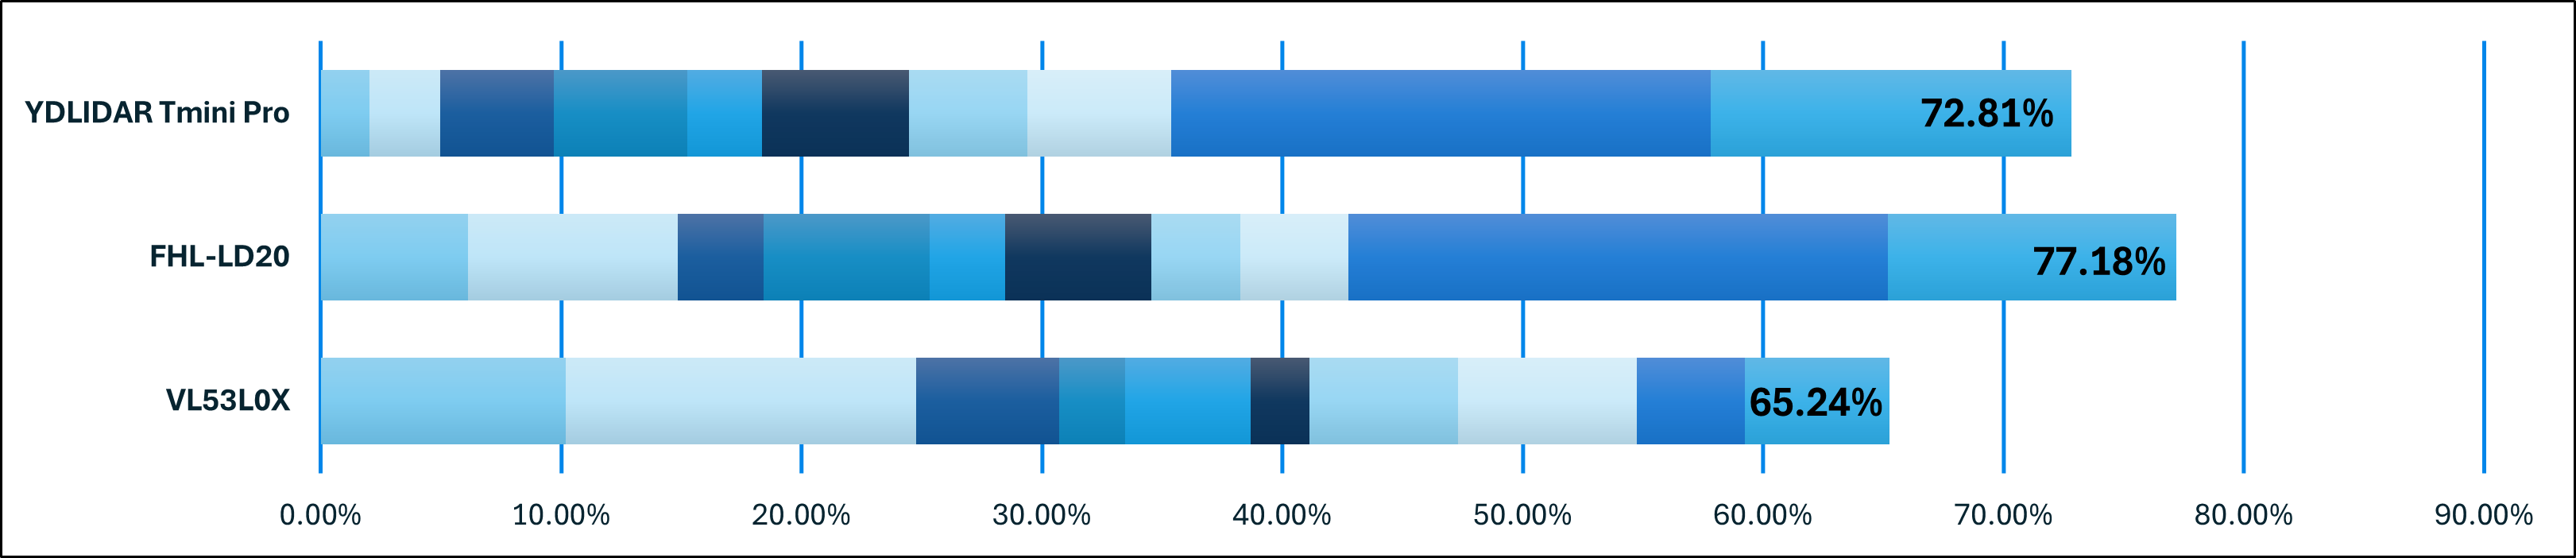
\includegraphics[width=1\textwidth]{trade_study.png}
	\caption{Resultados del \textit{trade study}.}
	\label{fig:graf_trade_study}
\end{figure}

\begin{figure}[H]
	\centering
	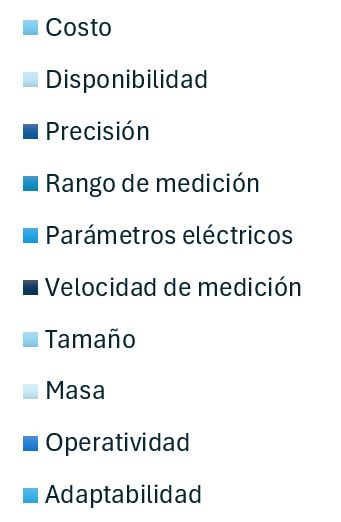
\includegraphics[width=0.25\textwidth]{parametros_tradestudy.jpg}
	\caption{Leyenda del gráfico de barras segmentadas.}
	\label{fig:legend_graf_trade_study}
\end{figure}

\begin{table}[H]
	\centering
	\begin{tabular}{|l|r|r|r|}
		\hline
		\multirow{2}{6.5cm}{\centering\textbf{Criterios}}&\multicolumn{1}{|c|}{\textbf{VL53L0X}}&\multicolumn{1}{|c|}{\textbf{FHL-LD20}}&\multicolumn{1}{|c|}{\textbf{\makecell{YDLIDAR\\Tmini Pro}}}\\
		\cline{2-4}
		&\multicolumn{1}{|c|}{Pesos}&\multicolumn{1}{|c|}{Pesos}&\multicolumn{1}{|c|}{Pesos}\\
		
		\hline
		Costo&$10.19\%$&$6.11\%$&$2.04\%$\\
		\hline
		Disponibilidad&$14.57\%$&$8.74\%$&$2.91\%$\\
		\hline
		Precisión&$5.94\%$&$3.56\%$&$4.75\%$\\
		\hline
		Rango de medición&$2.76\%$&$6.91\%$&$5.53\%$\\
		\hline
		Parámetros eléctricos&$5.22\%$&$3.13\%$&$3.13\%$\\
		\hline
		Velocidad de medición&$2.44\%$&$6.09\%$&$6.09\%$\\
		\hline
		Tamaño&$6.17\%$&$3.70\%$&$4.94\%$\\
		\hline
		Masa&$7.46\%$&$4.48\%$&$5.97\%$\\
		\hline
		Operatividad en aplicaciones deseadas&$4.49\%$&$22.44\%$&$22.44\%$\\
		\hline
		Adaptabilidad a robots móviles&$6.00\%$&$12.00\%$&$15.00\%$\\
		\hline
		\multicolumn{1}{|r|}{\textbf{Total}}&\textbf{$65.24\%$}&\textbf{$77.18\%$}&\textbf{$72.81\%$}\\
		\hline
	\end{tabular}
	\caption{Ponderación individual de los sensores evaluados según criterios establecidos.} 
	\label{cuadro:ponderacion_individual}
\end{table}

\chapter{Lectura e interpretación de datos extraídos del LiDAR FHL-LD20}
Este capítulo aborda el funcionamiento y la interpretación de datos del sensor LiDAR FHL-LD20. Se detalla el formato de los paquetes de datos enviados por el sensor, y se describe cómo se captura y procesa esta información utilizando software como Matlab y Python. Además, se presenta la aplicación desarrollada para que el usuario comprenda como operar el sensor y utilizar de manera efectiva los datos que proporciona.

\section{Funcionamiento del sensor de distancia FHL-LD20}
Esta sección se centra en el funcionamiento del sensor FHL-LD20, detallando sus características técnicas, protocolo de comunicación y la estructura de los datos que transmite. Se exploran los principios de operación que permiten al sensor capturar y transmitir información de manera eficiente. La comprensión de estos aspectos es fundamental para integrar y utilizar el sensor de manera efectiva en aplicaciones que requieran mediciones precisas. 
\subsection{Características generales}
El sensor de distancia tipo láser FHL-LD20, fabricado por Youyeetoo, está diseñado para capturar datos en un plano bidimensional, generalmente en orientación horizontal. Utiliza un láser infrarrojo con una longitud de onda que varía entre 775 nm y 800 nm, siendo 793 nm el valor típico. Su campo de visión (FOV, por sus siglas en inglés) abarca una sección circular de 360° con un radio que varía entre 100 mm y 8 m. Además, cuenta con un motor eléctrico integrado que hace girar la ventana óptica de emisión y recepción del láser, permitiendo cubrir un ángulo de medición en todo el plano horizontal. En el Cuadro \ref{cuadro:parametrosrendi} se presentan a algunos parámetros relevantes del sensor.

\begin{table}[H]
	\centering
	\begin{tabular}{|l|l|} 
		\hline
		\multicolumn{2}{|c|}{Parámetros de rendimiento}\\
		\hline
		\multicolumn{1}{|l|}{Resolución angular}& 0.54°\\
		\hline
		\multicolumn{1}{|l|}{\textit{Pitch}}& 0°$\sim$1.0°\\
		\hline		
		\multicolumn{1}{|l|}{\textit{Yaw}}& -0.5°$\sim$0.5°\\
		\hline
		\multirow{2}{*}{Tiempo de arranque}&$\leq$ 3.4 s\\
		&Típico de 3 s\\
		\hline
		\multicolumn{1}{|l|}{Frecuencia de escaneo}& 6 Hz $\pm$ 0.2 Hz\\
		\hline
		\multicolumn{1}{|l|}{Temperatura de funcionamiento}& -10°C a 50°C\\
		\hline
		\multicolumn{1}{|l|}{Humedad relativa}& < 95\% RH\\
		\hline
		\multicolumn{1}{|l|}{Nivel de seguridad del láser}& IEC 60825 Clase 1\\
		\hline
	\end{tabular}
	\caption{Parámetros de rendimiento.} 
	\label{cuadro:parametrosrendi}
\end{table}

\subsubsection{Orientación del sensor}
El LiDAR FHL-LD20 utiliza un sistema de coordenadas zurdo, donde el centro de rotación actúa como el origen de coordenadas (ver Figura \ref{fig:orientación}). La dirección que conecta el centro de rotación con el centro de la rueda motriz se establece como la dirección de cero grados, y el ángulo de rotación aumenta en sentido horario. Ademas, el sensor tiene un margen limitado de inclinación y rotación en los ejes de \textit{pitch} y \textit{yaw}, por lo que si se superan los límites descritos en el Cuadro \ref{cuadro:parametrosrendi}, su capacidad para medir distancias con precisión podría verse comprometida.

\begin{figure}[H]
	\centering
	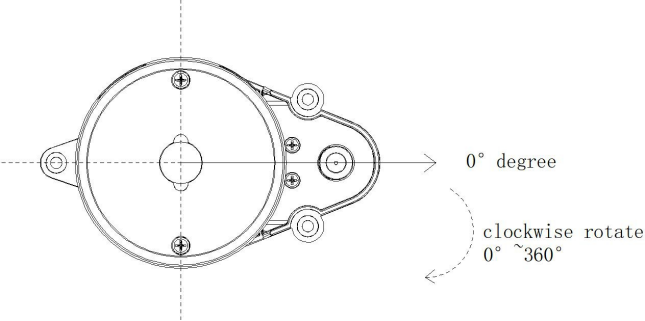
\includegraphics[width=0.7\textwidth]{orientacion_lidar.jpg}
	\caption{Orientación del sensor \cite{youyeetoo_tech_ld20_nodate}.}
	\label{fig:orientación}
\end{figure}

\subsection{Protocolo de comunicación}
El FHL-LD20 utiliza un puerto serial asíncrono estándar (UART) para la transmisión unidireccional de datos. La conexión se realiza a través de un conector ZH1.5T-4P de 1.25mm, que se utiliza tanto para la alimentación como para la transmisión de datos hacia un dispositivo \textit{Host}. En la Figura \ref{fig:pines} y en el Cuadro \ref{cuadro:parametrostrans} se muestra el orden de los pines de entrada y salida del sensor, y en el Cuadro \ref{cuadro:parametrostrans} se especifican los parámetros de transmisión.

\begin{figure}[H]
	\centering
	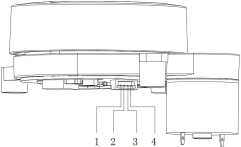
\includegraphics[width=0.4\textwidth]{pin_lidar.jpg}
	\caption{Esquema de conexión del conector ZH1.5T-4P del LiDAR FHL-LD20 \cite{youyeetoo_tech_ld20_nodate}.}
	\label{fig:pines}
\end{figure}

\begin{table}[H]
	\centering
	\resizebox{\textwidth}{!}{\begin{tabular}{|l|l|l|l|l|l|l|} 
		\hline
		\multirow{2}{*}{\centering\textbf{No. Pin}}&\multirow{2}{*}{\centering\textbf{Señal}}&\multirow{2}{*}{\centering\textbf{Tipo}}&\multirow{2}{*}{\centering\textbf{Descripción}}&\multicolumn{3}{|c|}{\textbf{Voltajes de operación}}\\
		&&&&\multicolumn{1}{|c|}{\textbf{Mínimo}}&\multicolumn{1}{|c|}{\textbf{Típico}}&\multicolumn{1}{|c|}{\textbf{Máximo}}\\
		\hline
		\multicolumn{1}{|c|}{\textbf{1}}&RX/PWM&Entrada&Control de velocidad externo&3 V&3.3 V&3.6 V\\
		\hline
		\multicolumn{1}{|c|}{\textbf{2}}&GND&Alimentación&Tierra&-&0 V&-\\
		\hline
		\multicolumn{1}{|c|}{\textbf{3}}&TZ&Salida&Salida de datos del LiDAR&3 V&3.3 V&3.6 V\\
		\hline
		\multicolumn{1}{|c|}{\textbf{4}}&VCC&Alimentación&Alimentación positiva&4.5 V&5 V&5.5 V\\
		\hline
	\end{tabular}}
	\caption{Parámetros de conexión del Lidar FHL-LD20.} 
	\label{cuadro:parametrospin}
\end{table}

\begin{table}[H]
	\centering
	\resizebox{\textwidth}{!}{\begin{tabular}{|l|l|l|l|l|} 
		\hline
		\multicolumn{1}{|c|}{\textbf{Velocidad en baudios}}&\multicolumn{1}{|c|}{\textbf{Longitud de los datos}}&\multicolumn{1}{|c|}{\textbf{Bits de parada}}&\multicolumn{1}{|c|}{\textbf{Bit de paridad}}&\multicolumn{1}{|c|}{\textbf{Control de flujo}}\\
		\hline
		230400&8 bits&1&N/A&N/A\\
		\hline
	\end{tabular}}
	\caption{Parámetros de transmisión UART.} 
	\label{cuadro:parametrostrans}
\end{table}

\subsubsection{Formato de paquete}
Cuando el sensor alcanza un estado de operación estable, comienza a enviar automáticamente paquetes de datos de medición sin requerir ninguna instrucción. En el Cuadro \ref{cuadro:paquete} se detalla la estructura general de estos paquetes de medición y el significado de cada campo.
\begin{table}[H]
	\centering
	\resizebox{\textwidth}{!}{\begin{tabular}{|l|l|l|l|l|l|l|l|l|l|l|l|} 
			\hline
			\multicolumn{1}{|c|}{\textbf{\makecell{Carácter\\de inicio}}}&\multicolumn{1}{|c|}{\textbf{VerLen}}&\multicolumn{2}{|c|}{\textbf{\makecell{Velocidad\\del radar}}}&\multicolumn{2}{|c|}{\textbf{\makecell{Ángulo\\de inicio}}}&\multicolumn{1}{|c|}{\textbf{Data}}&\multicolumn{2}{|c|}{\textbf{\makecell{Ángulo\\final}}}&\multicolumn{2}{|c|}{\textbf{\makecell{Marca\\de tiempo}}}&\multicolumn{1}{|c|}{\textbf{\makecell{Verificación\\CRC}}}\\
			\hline
			54H&2CH&LSB&MSB&LSB&MSB&...&LSB&MSB&LSB&MSB&1 Byte\\
			\hline
			\multicolumn{12}{c}{\textbf{}}\\
			\multicolumn{6}{c}{\textbf{}}&\multicolumn{1}{c}{\textbf{$\Downarrow$}}&\multicolumn{5}{c}{\textbf{}}\\
			\multicolumn{12}{c}{\textbf{}}\\
			\hline
			\multicolumn{3}{|c|}{\textbf{Punto de medición 1}}&\multicolumn{3}{|c|}{\textbf{Punto de medición 2}}&\multicolumn{3}{|c|}{\textbf{...}}&\multicolumn{3}{|c|}{\textbf{Punto de medición 12}}\\
			\hline
			\multicolumn{2}{|c|}{\textbf{Valor distancia 1}}&\textbf{Intensidad}&\multicolumn{2}{|c|}{\textbf{Valor distancia 2}}&\textbf{Intensidad}&\multicolumn{3}{|c|}{\textbf{...}}&\multicolumn{2}{|c|}{\textbf{Valor distancia 12}}&\textbf{Intensidad}\\
			\hline
			LSB&MSB&1 Byte&LSB&MSB&1 Byte&\multicolumn{3}{|c|}{\textbf{...}}&LSB&MSB&1 Byte\\
			\hline
	\end{tabular}}
	\caption{Estructura de un paquete de medición.} 
	\label{cuadro:paquete}
\end{table}

\begin{itemize}
	\item  Carácter de inicio (1 byte): Valor fijo de 0x54, señala el inicio de un paquete.
	\item  VerLen (1 byte): Valor fijo de 0x2C, especifica que cada paquete contiene 12 puntos de medición.
	\item  Velocidad del radar (2 bytes): Representa la velocidad del radar en grados por segundo.
	\item  Ángulo de inicio (2 bytes): Indica el ángulo de inicio en unidades de 0.01 grados.
	\item  Data (36 bytes): Contiene la información de 12 puntos de medición, cada uno de 3 bytes. Los primeros 2 bytes de cada punto indican el valor de distancia en milímetros, y el tercer byte refleja la intensidad de la señal de reflexión; los valores más altos indican una mayor intensidad.
	\item  Ángulo final (2 bytes): Señala el ángulo de finalización de la medición, en unidades de 0.01 grados.
	\item  Marca de tiempo (2 bytes): Representa el tiempo en milisegundos en el que se capturaron los datos.
	\item  Verificación CRC (1 byte):  Byte utilizado como \textit{checksum} para asegurar la integridad de todos los datos anteriores que forman un phaquete.
\end{itemize}

\section{Lectura de datos}
La integración de microcontroladores y software de análisis es fundamental para el desarrollo de sistemas de captura y procesamiento de datos en aplicaciones de sensores. En esta sección, se describe el proceso de lectura y decodificación de datos del sensor FHL-LD20, utilizando un microcontrolador ESP32 y plataformas de software como Matlab y Python. También, se presenta la aplicación desarrollada para la recolección e interpretación de datos del sensor, proporcionando una herramienta útil para evaluar su precisión y confiabilidad en diversos escenarios.

\subsection{Lectura e interpretación de datos mediante ESP32 y Matlab}
Para desarrollar el prototipo inicial de un sistema de captura y análisis de datos del sensor FHL-LD20, se utilizó un microncontrolador ESP32, programado mediante la plataforma de Arduino, en combinación con el software Matlab. El microcontrolador ESP32 se encargó de la recolección de información a través de la conexión UART proporcionada por el sensor. Este primer modelo permitió realizar una evaluación preliminar del rendimiento del sensor. En la Figura \ref{fig:diagrama_captura} se muestra el proceso general de captura de datos en términos generales.

\begin{figure}[H]
	\centering
	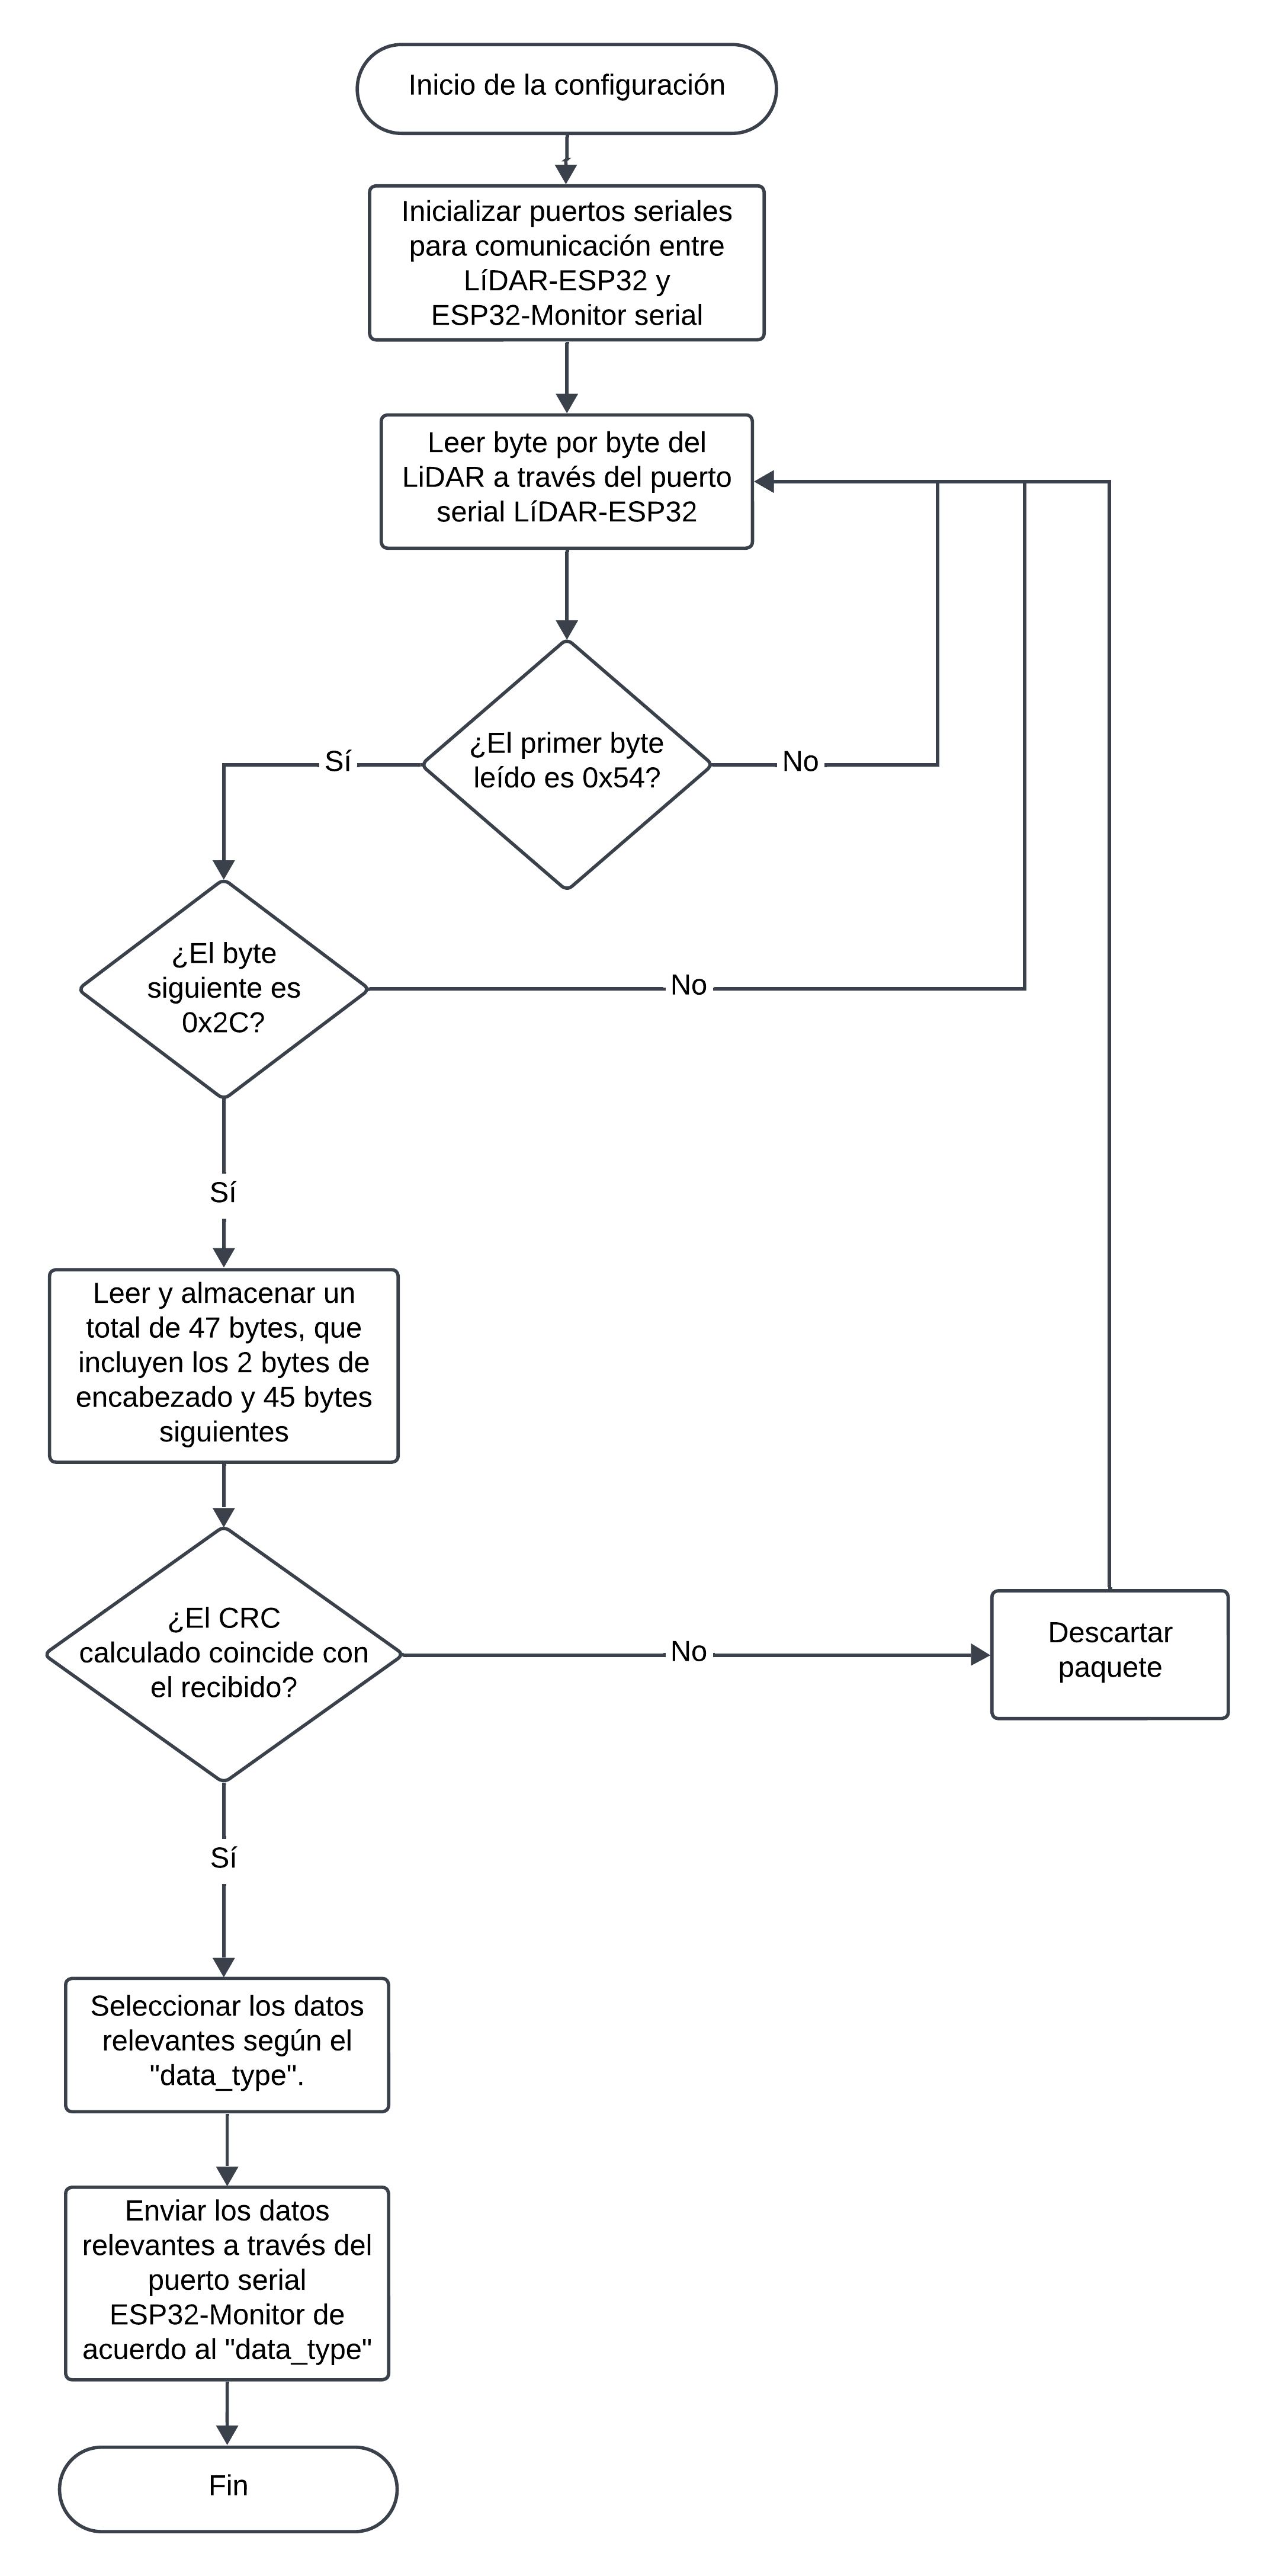
\includegraphics[width=0.6\textwidth]{diagrama_captura.png}
	\caption{Diagrama de flujo general para captura de datos provenientes del sensor.}
	\label{fig:diagrama_captura}
\end{figure}

El proceso de captura de datos sigue una estructura de validación en la que se espera recibir un paquete de 47 bytes. Cada paquete se valida mediante los dos bytes de encabezados específicos (0x54 y 0x2C), una vez recibido el paquete completo, se realiza una verificación de integridad utilizando un cálculo de verificación por redundancia cíclica (CRC) de 8 bits. El código opera de manera cíclica en el bucle principal, lo que permite un flujo continuo de lectura de datos del LiDAR. 

En el diagrama de flujo presentado se destaca la importancia de la variable ``data\_type''. Esta variable define la cantidad de datos que el microcontrolador enviará a Matlab para su procesamiento. Dicha variable puede asumir uno de tres valores predefinidos: ``FULL\_DATA'', ``RELEVANT\_DATA'' o ``RELEVANT\_DATA2'', cada uno especificando una longitud distinta para los datos a transmitir.
\begin{itemize}
	\item  ``FULL\_DATA'': Corresponde a un paquete completo de 47 bytes (94 caracteres).
	\item ``RELEVANT\_DATA'': Paquete de 30 bytes que excluye la velocidad del radar, los bytes de intensidad de la señal, los de la marca de tiempo y el byte de verificación CRC (60 caracteres).
	\item ``RELEVANT\_DATA2'': Paquete de 42 bytes que, a diferencia de ``RELEVANT\_DATA'', incluye los bytes de intensidad de la señal (84 caracteres).
\end{itemize}
La flexibilidad en el tamaño de los paquetes fue implementada para optimizar el tiempo de procesamiento en Matlab, lo cual es particularmente relevante en aplicaciones en tiempo real o cuando se manejan múltiples paquetes de datos en rápida sucesión. Al reducir la cantidad de información procesada, se logra una respuesta más rápida del sistema sin necesidad de realizar cambios significativos en el software. Cabe destacar que los datos capturados se envían como una cadena de caracteres hexadecimales a través del puerto serial.

Una vez capturada la información del sensor, se utilizó Matlab para desarrollar un programa capaz de recibir los datos transmitidos desde el microcontrolador. El software permitió obtener y decodificar múltiples lecturas consecutivas, así como graficar los resultados. Este proceso se utilizó para verificar la concordancia de las lecturas del sensor con los valores esperados, además de ofrecer una herramienta sencilla para manipular los datos recibidos. La Figura \ref{fig:diagrama_procesamiento} muestra el proceso de recepción, decodificación y visualización de los datos obtenidos.

\begin{figure}[H]
	\centering
	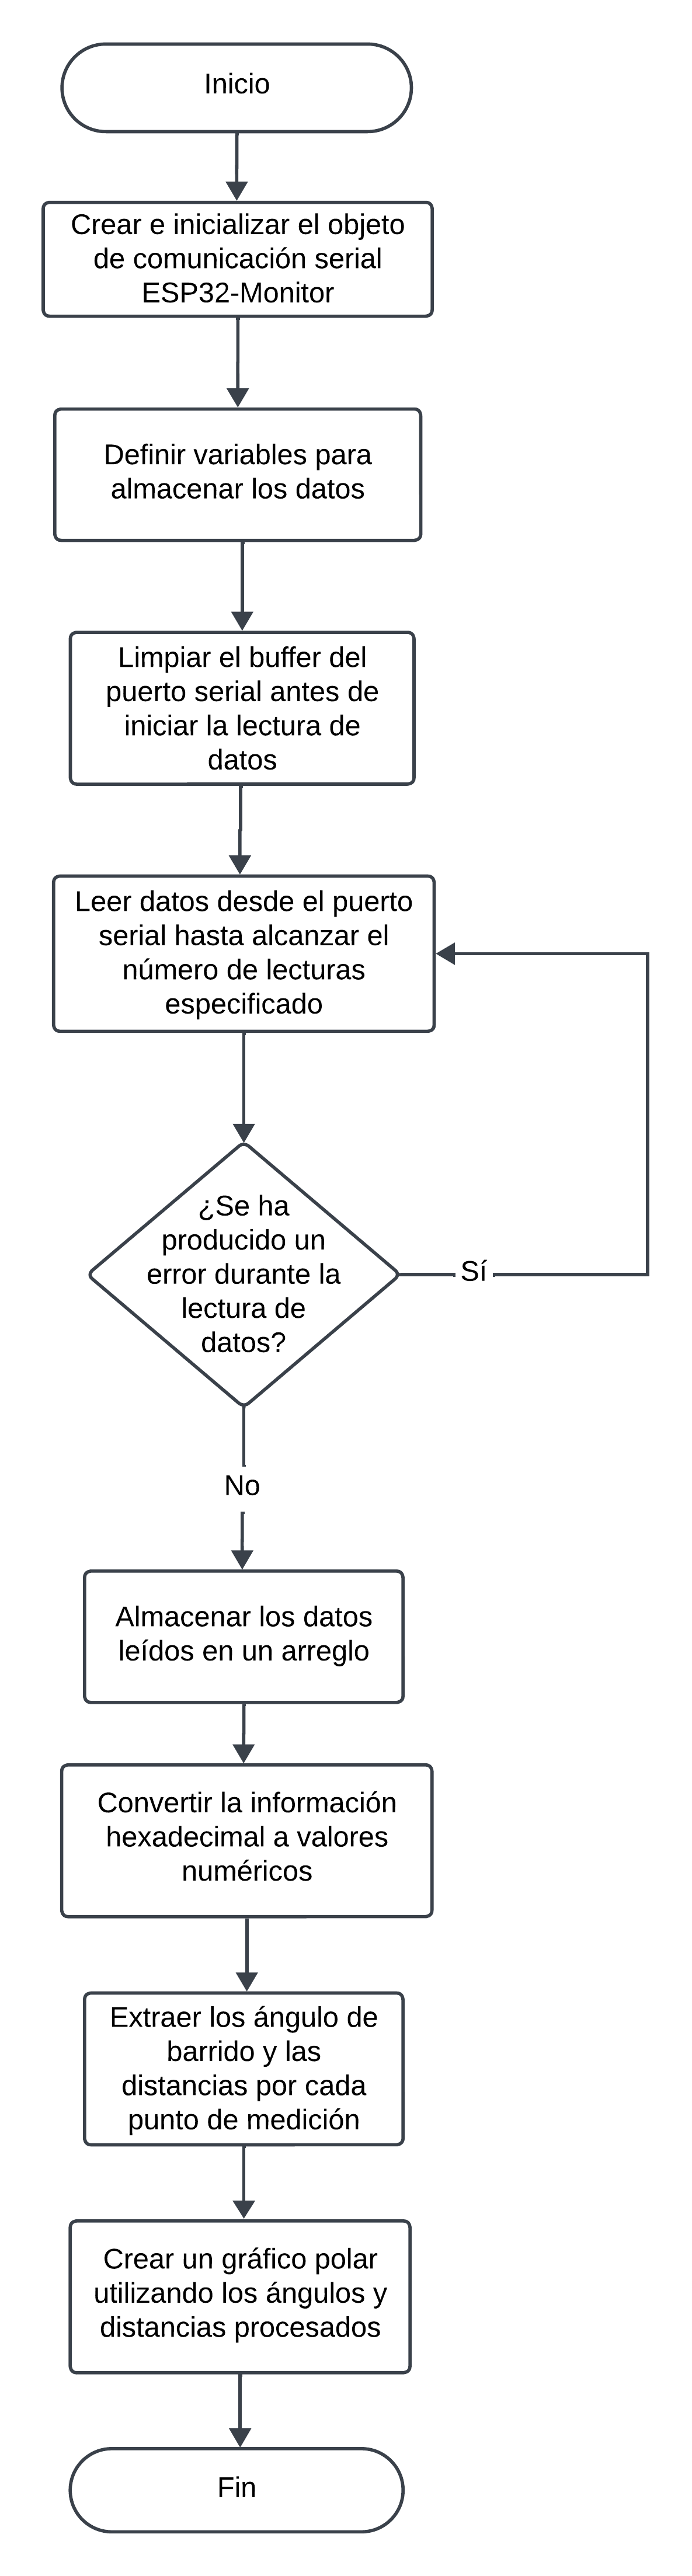
\includegraphics[width=0.33\textwidth]{diagrama_procesamiento.png}
	\caption{Diagrama de flujo general para procesamiento de datos provenientes del sensor.}
	\label{fig:diagrama_procesamiento}
\end{figure}

Como se mencionó anteriormente, el paquete de datos recibido consiste en un arreglo de caracteres que contiene información estructurada en formato hexadecimal. La conversión de datos se realiza dividiendo el paquete en segmentos y extrayendo pares de caracteres hexadecimales. Para reconstruir los valores completos de ángulos y distancias, se combinan dos partes: un byte de menor orden y un byte de mayor orden. 

Por ejemplo, para el ángulo de inicio codificado en dos bytes, se extraen las partes de menor y mayor orden para obtener los valores hexadecimales correspondientes. Luego, se desplaza el byte de mayor orden a la posición correcta dentro del valor de 16 bits y se suma con el byte de menor orden para obtener el valor completo. De esta manera, se reconstruye el valor decimal correspondiente al ángulo de inicio medido, expresado en unidades de 0.01 grados, en el paquete de datos evaluado como se muestra en la Figura \ref{fig:data_in}.

\begin{figure}[H]
	\centering
	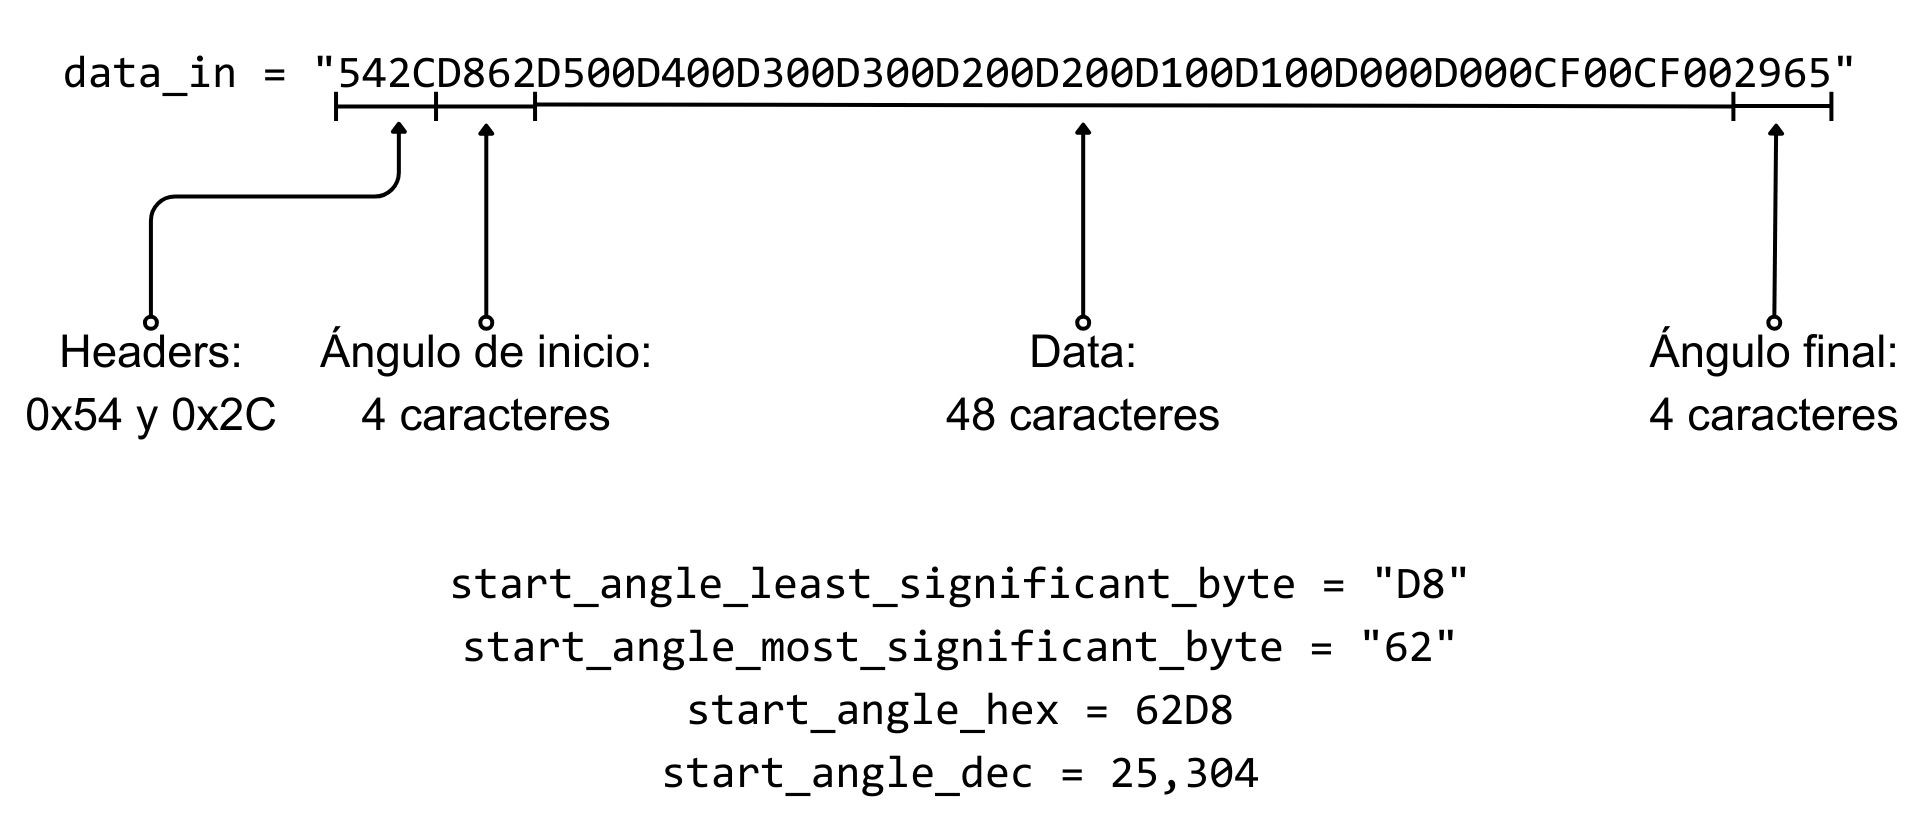
\includegraphics[width=0.8\textwidth]{data_in.jpg}
	\caption{Ejemplificación del proceso de reconstrucción de mediciones: ángulo de inicio.}
	\label{fig:data_in}
\end{figure}

Una vez que las lecturas fueron decodificadas y segmentadas en sus partes correspondientes, se calculó el ángulo de barrido para cada punto de distancia. Este cálculo se realizó determinando el paso angular, el cual fue obtenido al dividir la diferencia entre los ángulos de inicio y fin por el número de intervalos entre los puntos de medición. Este incremento angular fue sumado acumulativamente al angulo de inicio. De esta manera, a cada punto de distancia medido se le asignaría un ángulo de barrido específico. Cabe destacar que la diferencia entre los ángulos de inicio y fin fue de aproximadamente 6°, lo que implica que cada paquete de datos cubre un barrido de esta magnitud.

Los valores de distancias y ángulos resultantes del procesamiento de datos se organizaron en una matriz de datos la cual se representó en una gráfica de coordenadas polares en Matlab para recrear la visualización generada por el LiDAR. Para verificar su funcionamiento y realizar un reconocimiento de área, se colocó el sensor FHL-LD20 dentro de una caja de 38.5$\times$23 cm. En la Figura \ref{primera_corrida} se presenta la disposición del sensor dentro de la caja y la reconstrucción visual realizada a partir de 60 paquetes del puerto serial, es decir, 720 puntos de medición procesados o bien, una revolución completa.

\begin{figure}[H]
	\centering
	\begin{subfigure}{0.8\textwidth}
		\centering
		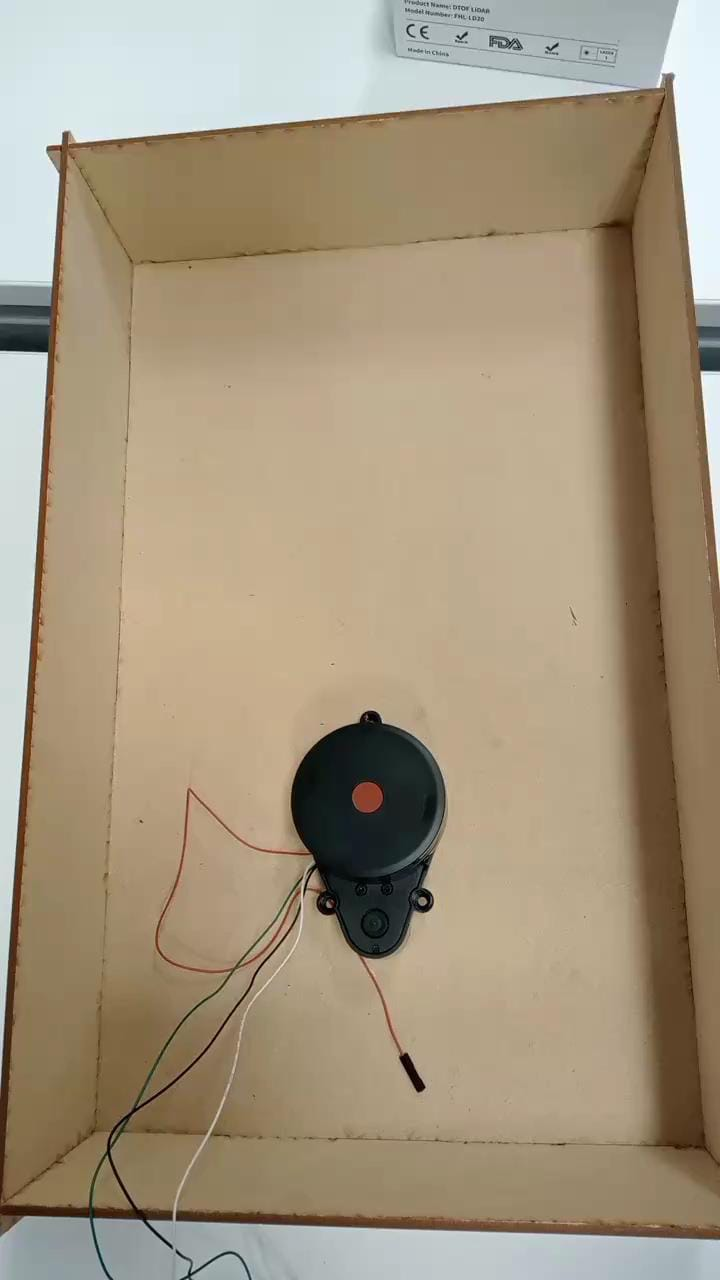
\includegraphics[angle=270,width=0.8\linewidth]{disposicion_lidar1.jpeg}
		\caption{Disposición del sensor FHL-LD20 dentro de la caja.}
		\label{primera_corrida_disp}
		\vspace{1em}
	\end{subfigure}
	\begin{subfigure}{0.8\textwidth}
		\centering
		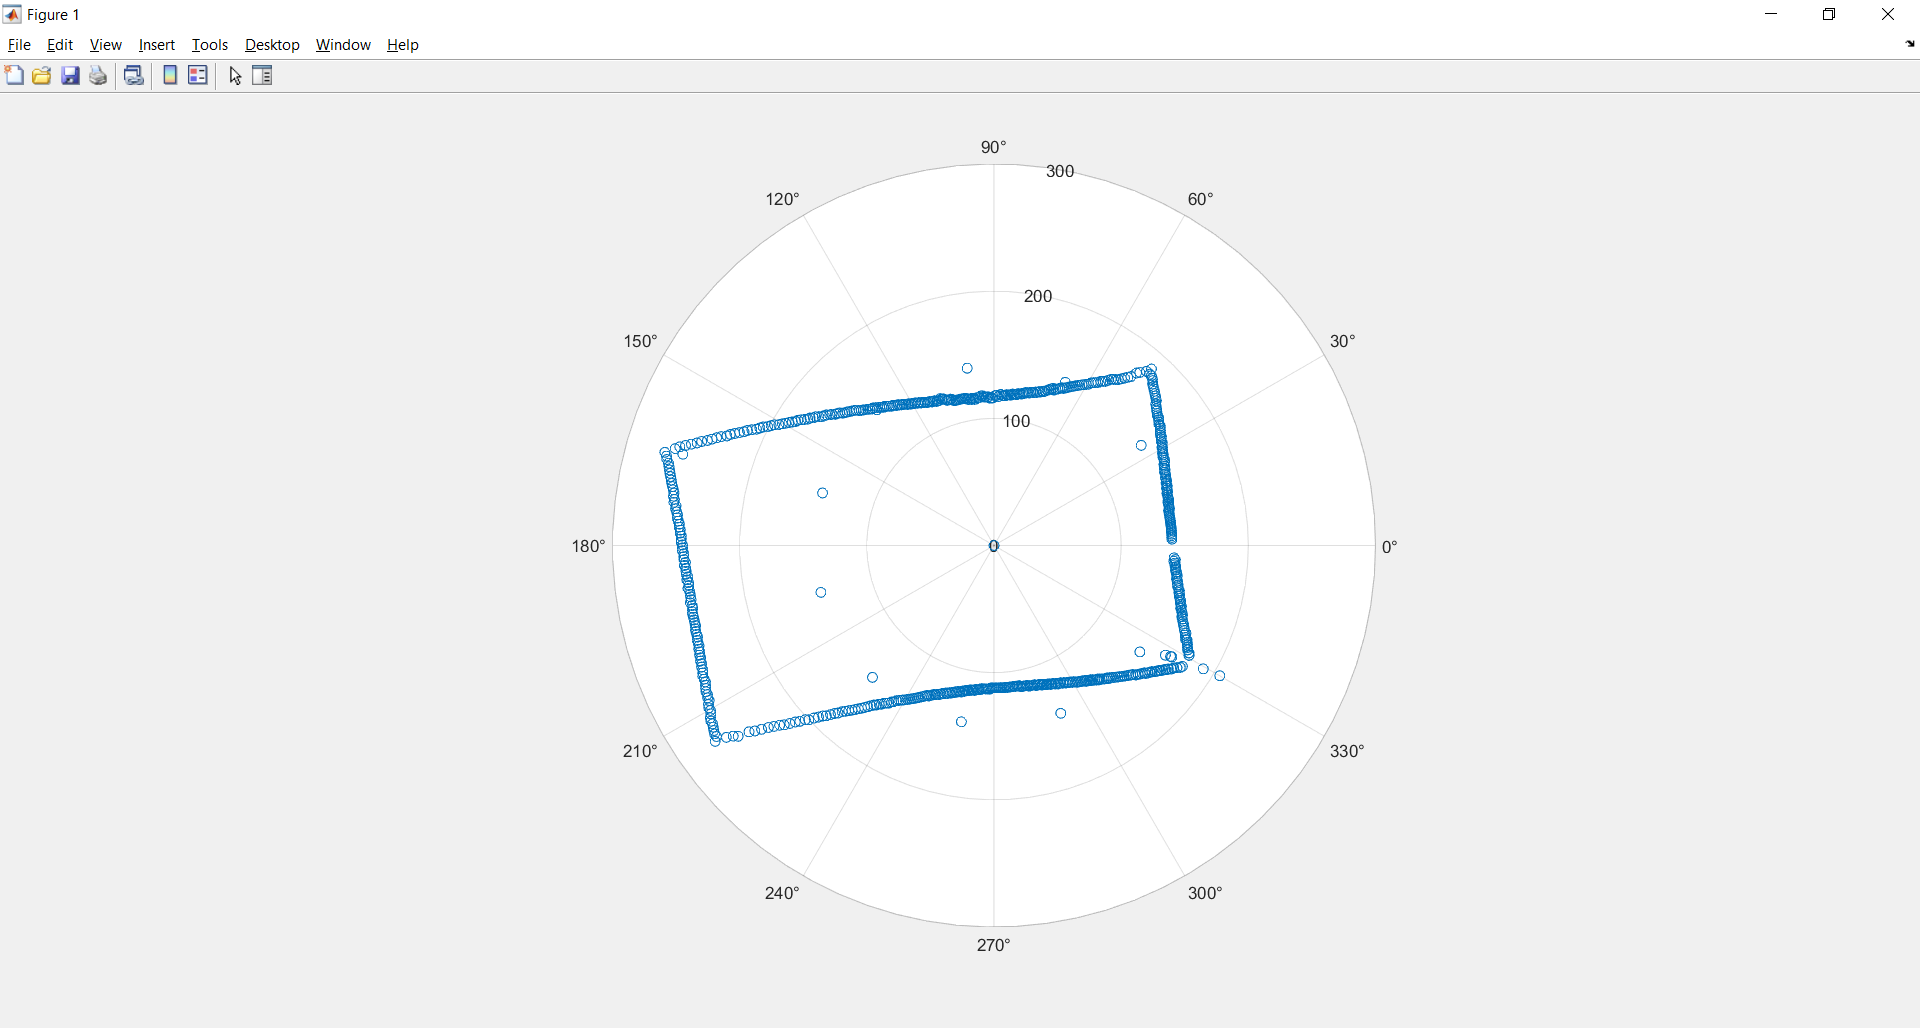
\includegraphics[width=0.8\linewidth]{primera_lectura.png}
		\caption{Reconstrucción de las 70 lecturas del sensor.}
		\label{primera_corrida_recon}
	\end{subfigure}
	\caption{Visualización de la primera corrida del sensor: 840 puntos de medición.}
	\label{primera_corrida}
\end{figure}
A partir de la Figura \ref{primera_corrida_recon}, se identificaron distintas áreas de mejora al momento de realizar la reconstrucción. En primer lugar, aunque la forma y las proporciones generales de la caja se representaron correctamente, la reconstrucción se presenta de manera ``invertida'' en comparación con la disposición física observada (Figura \ref{primera_corrida_disp}). La causa de esta discrepancia radica en que el LiDAR captura los datos en dirección horaria, mientras que los sistemas de visualización convencionales suelen interpretar los datos en sentido antihorario. Como resultado, la orientación visual de la reconstrucción difiere con lo que se observa a simple vista. Este hecho resaltó la necesidad de implementar una opción para ajustar la orientación de los puntos capturados, de modo que la reconstrucción se alinee con la disposición física y sea más intuitiva.

Otro aspecto destacable es la ligera curvatura observada en las aristas de la reconstrucción, que difiere con los bordes rectos de la caja física. Esta distorsión surgió debido a que los datos se procesaron sin considerar el ajuste para alinear los puntos obtenidos con el sistema de referencia deseado (eje central de rotación del sensor como origen). Es decir, no se aplicó una compensación adecuada para corregir los desfases entre el sistema de coordenadas en el que se capturan las mediciones (propio del LiDAR) y el sistema de coordenadas en el que se deberían de visualizar los datos (eje central). Como resultado, la reconstrucción presenta una leve deformación en comparación con la realidad física observada.

Además, se identificó un conjunto de aproximadamente 10 puntos distribuidos de forma circular que no deberían de estar presentes en la reconstrucción. Al revisar el procesamiento de datos, se determinó que estos puntos atípicos surgieron debido a un error en el cálculo del barrido angular. Cuando el ángulo de inicio era mayor que el ángulo final, se obtenía una diferencia negativa, lo que provocaba que las mediciones cercanas al cruce del punto de 0 grados se distorsionaran. Para solventar esto, se implementó una corrección en el cálculo del ángulo, añadiendo 360 grados cuando el ángulo de inicio superaba al ángulo final. Esta corrección garantizaba una transición continua entre mediciones al momento en que el sensor completaba un ciclo y cruzaba por el ángulo de 0 grados. Estos detalles no solo resaltaron la importancia de revisar cuidadosamente el procesamiento de datos, sino también la necesidad de diseñar un soporte para estabilizar y alinear adecuadamente el sensor LiDAR.

\subsection{Lectura e interpretación de datos mediante ESP32 y Python}
En lugar de desarrollar únicamente un software para obtener y procesar los datos, se decidió crear una aplicación que mejorara la experiencia del usuario al utilizar el sensor FHL-LD20. Para ello, se optó por utilizar Python 3.11 como lenguaje de programación, considerando la necesidad de un entorno más flexible y eficiente para el manejo de datos. Las principales razones por las cuales se seleccionó Python sobre Matlab, que se había usado anteriormente, fueron las siguientes:
\begin{itemize}
	\item  A diferencia de Matlab, Python es un lenguaje de código abierto y gratuito. 
	\item Python cuenta con un ecosistema amplio, con una gran variedad de librerías y \textit{frameworks} que facilitan la integración de diferentes funcionalidades en una misma aplicación.
	\item Para el desarrollo de aplicaciones de escritorio, Python ofrece múltiples frameworks como Tkinter, PyQT y Kivy, mientras que Matlab sólo dispone de App Designer para la creación de interfaces gráficas.
	\item Python cuenta con una comunidad de desarrolladores muy grande y activa, lo que facilita la resolución de problemas y la implementación de nuevas funcionalidades.
\end{itemize}
Cabe señalar que el código desarrollado para el ESP32, se mantuvo sin cambios, ya que mostró ser eficiente para la recolección de datos.

Ahora bien, para el desarrollo de la aplicación, se empleó CustomTkinter, una extensión moderna y estilizada de Tkinter. Esta elección no solo permitió mejorar la estética de la interfaz, sino que también ofreció una experiencia más funcional en comparación con herramientas tradicionales, como Tkinter. En la Figura \ref{fig:vista_interfaz}, se presenta la interfaz gráfica nombrada ``LiDAR MapViewer'', junto con las distintas opciones y paneles disponibles dentro de la aplicación. Es importante destacar que el procesamiento de datos siguió la misma estructura general que el diagrama de flujo presentado en la Figura \ref{fig:diagrama_procesamiento}. Las modificaciones específicas realizadas se detallan en el siguiente capítulo.

\begin{figure}[H]
	\centering
	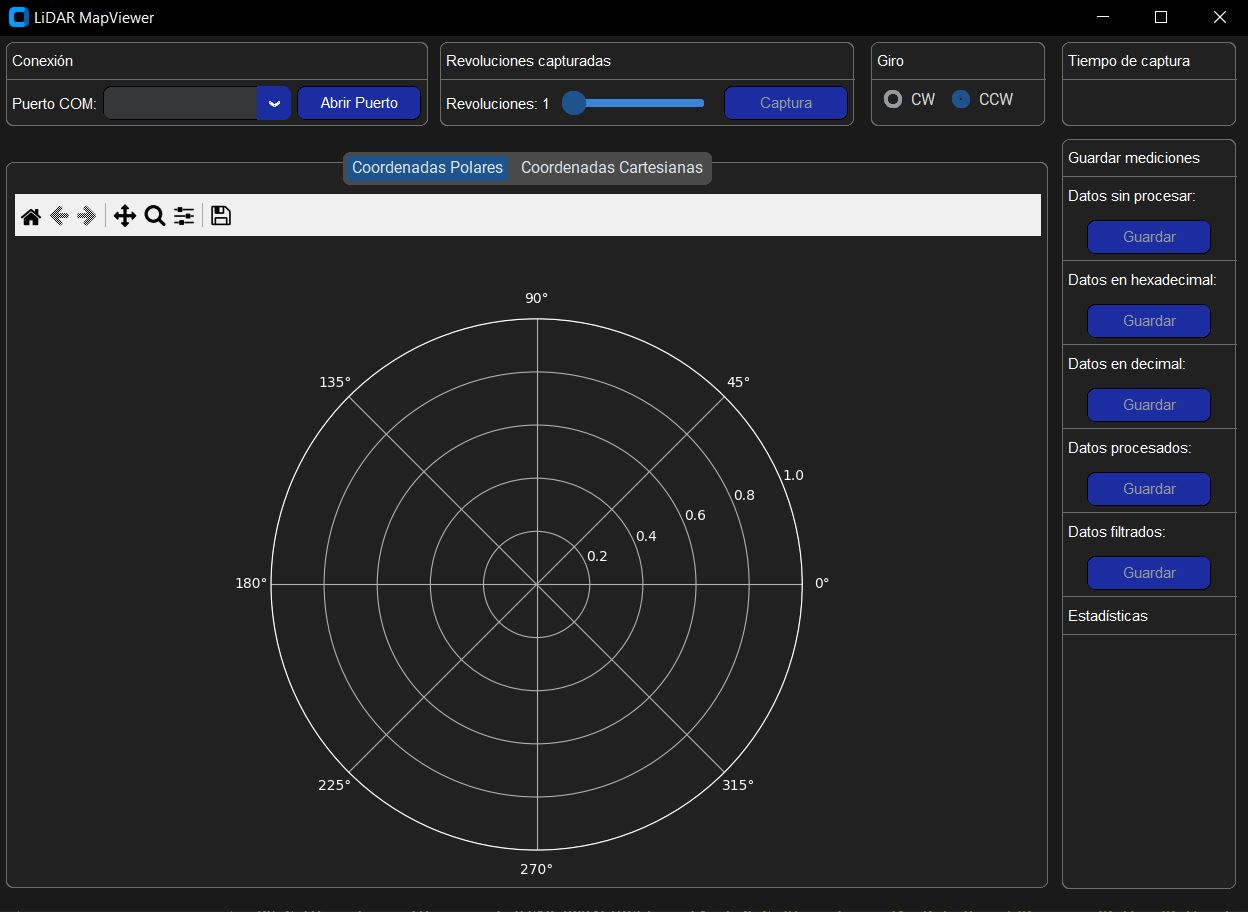
\includegraphics[width=0.9\textwidth]{app.jpg}
	\caption{Vista de usuario, interfaz gráfica LiDAR MapViewer.}
	\label{fig:vista_interfaz}
\end{figure}

\begin{itemize}
	\item  Panel de conexión: Este panel gestiona la conexión entre el ESP32 y el monitor a través de un puerto serial, que puede seleccionarse mediante un menú desplegable que muestra los puertos COM disponibles. La conexión se habilita mediante un botón, siempre que el puerto COM se encuentra activo y disponible. 
	\item Panel de revoluciones capturadas: Este marco contiene los controles para seleccionar y visualizar el número de revoluciones capturadas por el LiDAR. Incluye un control deslizante que permite elegir entre 1 y 5 revoluciones, y un botón para iniciar la captura de datos.
	\item Panel de giro: Este panel cuenta con dos botones que permiten al usuario seleccionar la orientación del giro  de los datos capturados por el LiDAR. Este selección ajusta el cálculo de los ángulos para su visualización.
	\item Panel de tiempo de captura: Muestra el tiempo total empleado por la interfaz para capturar, procesar y graficar todas las muestras seleccionadas por el usuario. El panel se actualiza al finalizar el proceso de captura.
	\item Panel de gráficos: Este marco contiene los gráficos de la interfaz, donde se visualizan los resultados de los datos capturados por el LiDAR, tanto en formato polar como cartesiano.
	\item Panel de guardado de mediciones: Este panel ofrece cinco opciones para almacenar distintos conjuntos de datos en archivos CSV:
	\begin{itemize}
		\item Datos sin procesar.
		\item Datos segmentados en hexadecimal.
		\item Datos segmentados en decimal.
		\item Datos procesados de ángulos y distancias.
		\item Datos filtrados de ángulos y distancias. 
	\end{itemize}
	Cada botón permite al usuario elegir la ubicación donde se guardará la información, simplificando así la organización y el análisis de los datos recopilados.
	\item Panel de pruebas estadísticas: Sección en la cual se muestran los análisis estadísticos de las mediciones radiales capturadas por el sensor. Esta sección solamente aplica para reconstrucciones de entornos circulares.
\end{itemize}

\chapter{Calibración del LiDAR FHL-LD20}
En este capítulo se describe la calibración del sensor LiDAR FHL-LD20, un proceso para corregir desviaciones sistemáticas en las lecturas, derivadas de factores inherentes del sensor, permitiendo que las mediciones reflejen con mayor fidelidad las dimensiones reales del entorno.  La calibración no solo minimiza discrepancias en distancia y ángulo, aspectos esenciales en aplicaciones como la navegación robótica y el mapeo, sino que también establece criterios de evaluación claros y parámetros clave para mejorar el procesamiento de datos. Este proceso resulta fundamental para garantizar la precisión y confiabilidad de las mediciones, alineándolas con un estándar o referencia conocida. Al combinarse con la caracterización del sensor, este procedimiento sienta las bases para un desempeño más robusto en filtros y algoritmos avanzados, optimizando la calidad de las mediciones y su interpretación.

\section{Desarrollo de plataforma física para pruebas y calibración del LiDAR FHL-LD20}
La plataforma para pruebas preliminares se diseñó utilizando el software de Autodesk Inventor 2024. La estructura consistía en una base cuadrada de 400$\times$400 mm sobre la cual se montaban cuatro paredes de 70 mm de altura de dos clases. Como se muestra en la Figura \ref{fig:pared_ranura}, la primera clase de pared presentaba divisiones escalonadas cada 10 mm, lo que permitía sujetar otras paredes y brindar modularidad a la plataforma. Esta pared también contaba con dos ranuras: una para deslizar y ajustar su posición sobre la plataforma, y otra para facilitar el paso de los cables de conexión del sensor. La segunda, en cambio, era una pieza sin divisiones (ver Figura \ref{fig:pared_normal}), diseñada para proporcionar soporte estructural adicional y cerrar la plataforma.

\begin{figure}[H]
	\centering
	\begin{subfigure}{0.5\textwidth}
		\centering	
		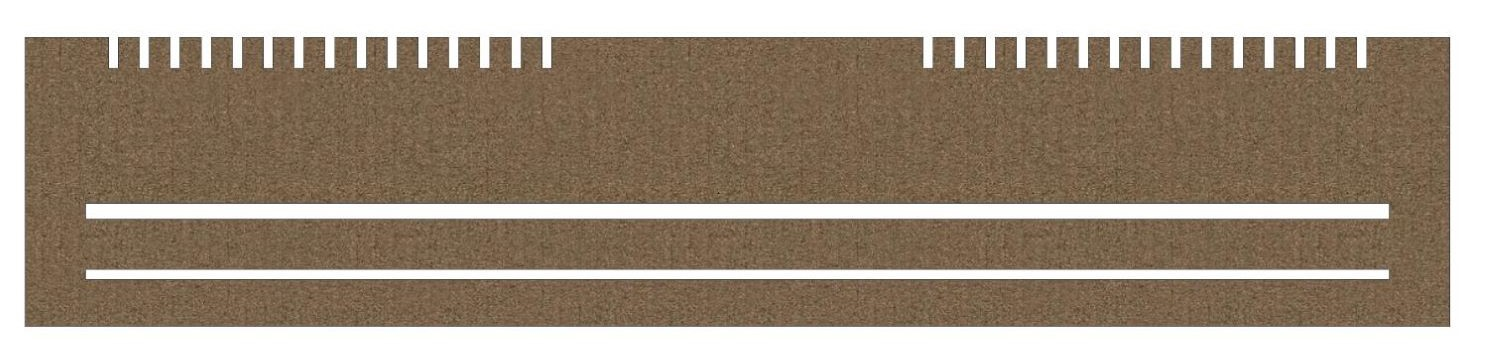
\includegraphics[width=1\linewidth]{pared_ranura.jpg}
		\caption{Pared modular con divisiones y ranuras.}
		\label{fig:pared_ranura}
	\end{subfigure}%
	\begin{subfigure}{0.5\textwidth}
		\centering
		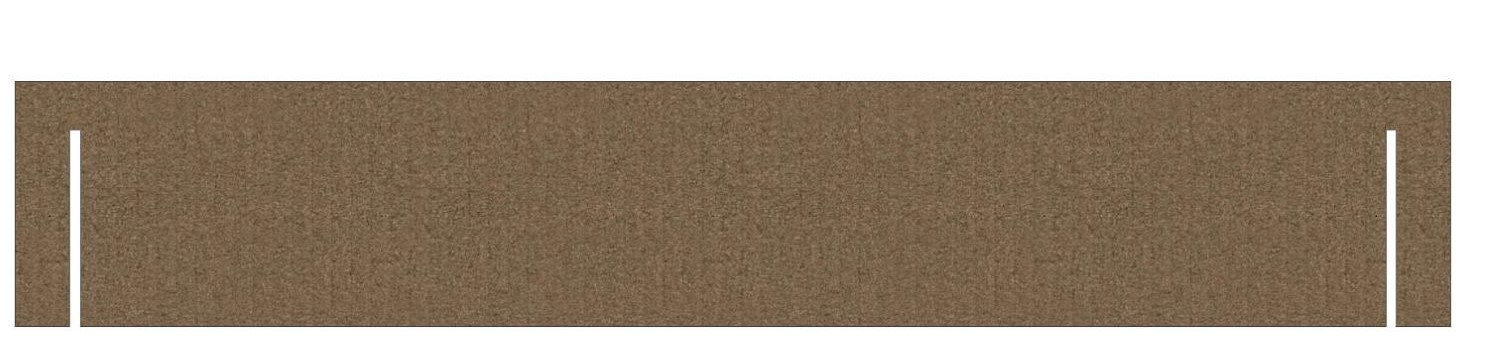
\includegraphics[width=1\linewidth]{pared_normal.jpg}
		\caption{Pared lisa de soporte estructural.}
		\label{fig:pared_normal}
	\end{subfigure}
	
	\caption{Vista frontal de las dos clases de paredes laterales que componen la plataforma de pruebas.}
	\label{fig:pared}
\end{figure}

En la Figura \ref{fig:base} se observa que la base de la plataforma fue cubierta con una cuadrícula milimetrada en la que se marcaron cuatro líneas diagonales a 45, 135, 225 y 315 grados. Esto se realizó con el objetivo de proporcionar referencias visuales precisas de las dimensiones de la plataforma para el montaje de las paredes y la alineación exacta del sensor en el espacio. Además, se diseñó un soporte para sujetar y nivelar el sensor, incorporando dos patrones radiales que simulaban una brújula (ver Figura \ref{fig:soporte}). Estos patrones se ubicaron a 135 y 225 grados desde el centro ideal del sensor, con un desplazamiento de 30 mm. Esta disposición permitió alinear el LiDAR correctamente, ya que, al estar su centro bloqueado visualmente, los patrones desplazados proporcionaban puntos de referencia para centrarlo con precisión, teniendo en cuenta la distancia radial de 30 mm y las diagonales de la base. 

\begin{figure}[H]
	\centering
	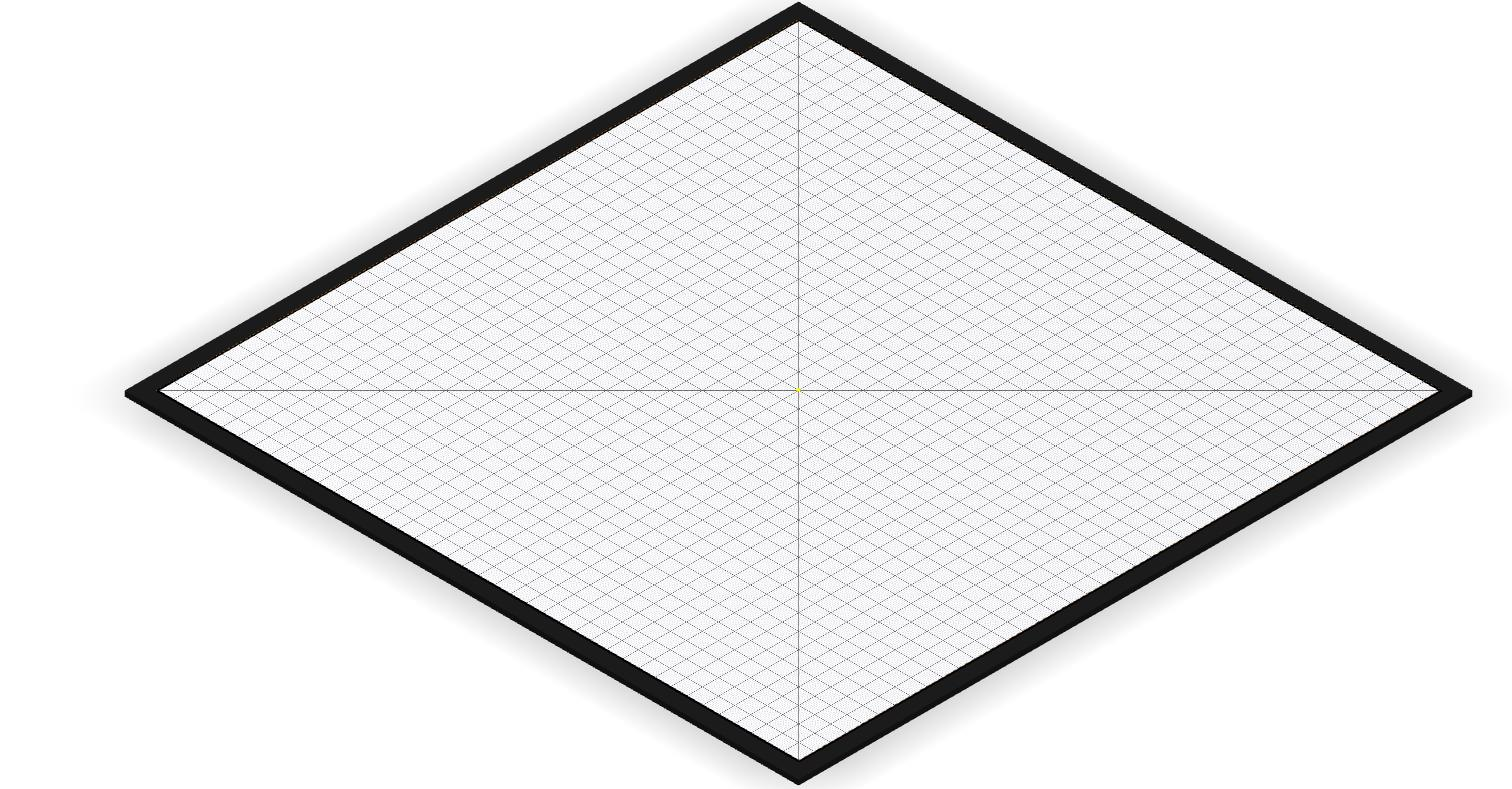
\includegraphics[width=0.6\textwidth]{base.jpg}
	\caption{Vista isométrica de la base de la plataforma de pruebas.}
	\label{fig:base}
\end{figure}

\begin{figure}[H]
	\centering
	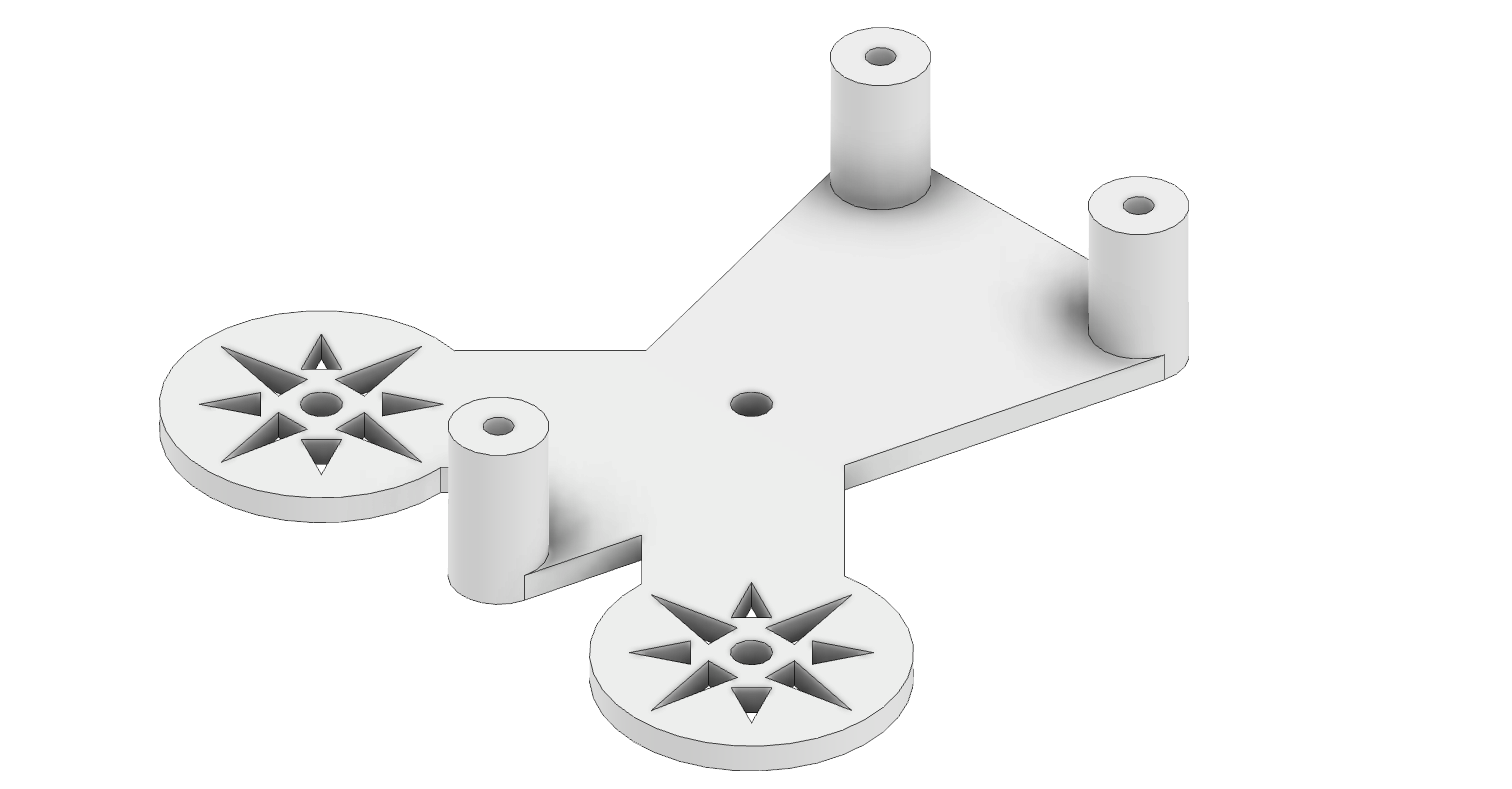
\includegraphics[width=0.5\textwidth]{base_lidar.png}
	\caption{Vista isométrica del soporte para el LiDAR FHL-LD20.}
	\label{fig:soporte}
\end{figure}

Las referencias visuales en la cuadrícula y las paredes de la plataforma permitieron comparar las lecturas obtenidas por el sensor con las dimensiones conocidas de la plataforma, ayudando a identificar cualquier desviación en las lecturas y permitiendo realizar ajustes en la orientación del sensor. Este escenario controlado aseguraba que cada medición del sensor fuera consistente y replicable en diversas pruebas. En la Figura \ref{fig:plataforma_pruebas} se presenta el diseño del ensamble final de la plataforma de pruebas, mientras que en la Figura \ref{fig:plataforma_fisica} se muestra la plataforma física fabricada junto con una reconstrucción visual del entorno, generada a partir de las lecturas del LiDAR tras el proceso de calibración descrito en la Sección \ref{sec:calibracion}.

\begin{figure}[H]
	\centering
	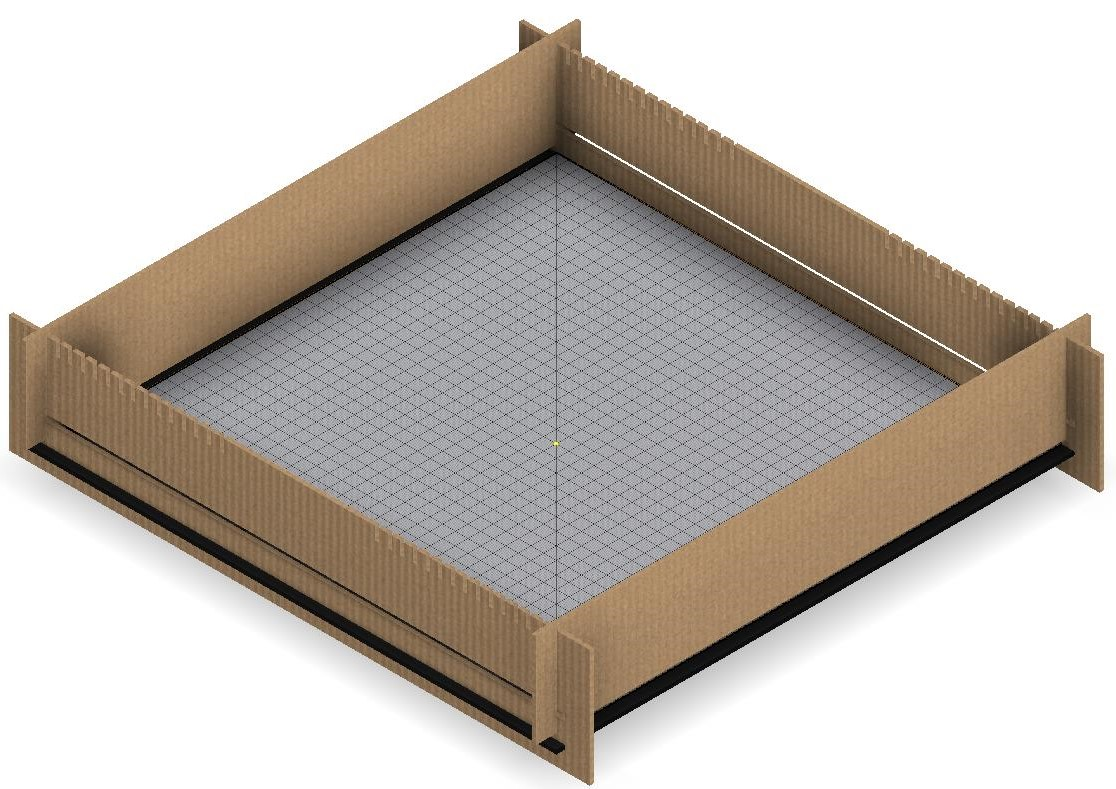
\includegraphics[width=0.6\textwidth]{plataforma_cad2.jpg}
	\caption{Vista isométrica de la plataforma de pruebas.}
	\label{fig:plataforma_pruebas}
\end{figure}

\begin{figure}[H]
	\centering
	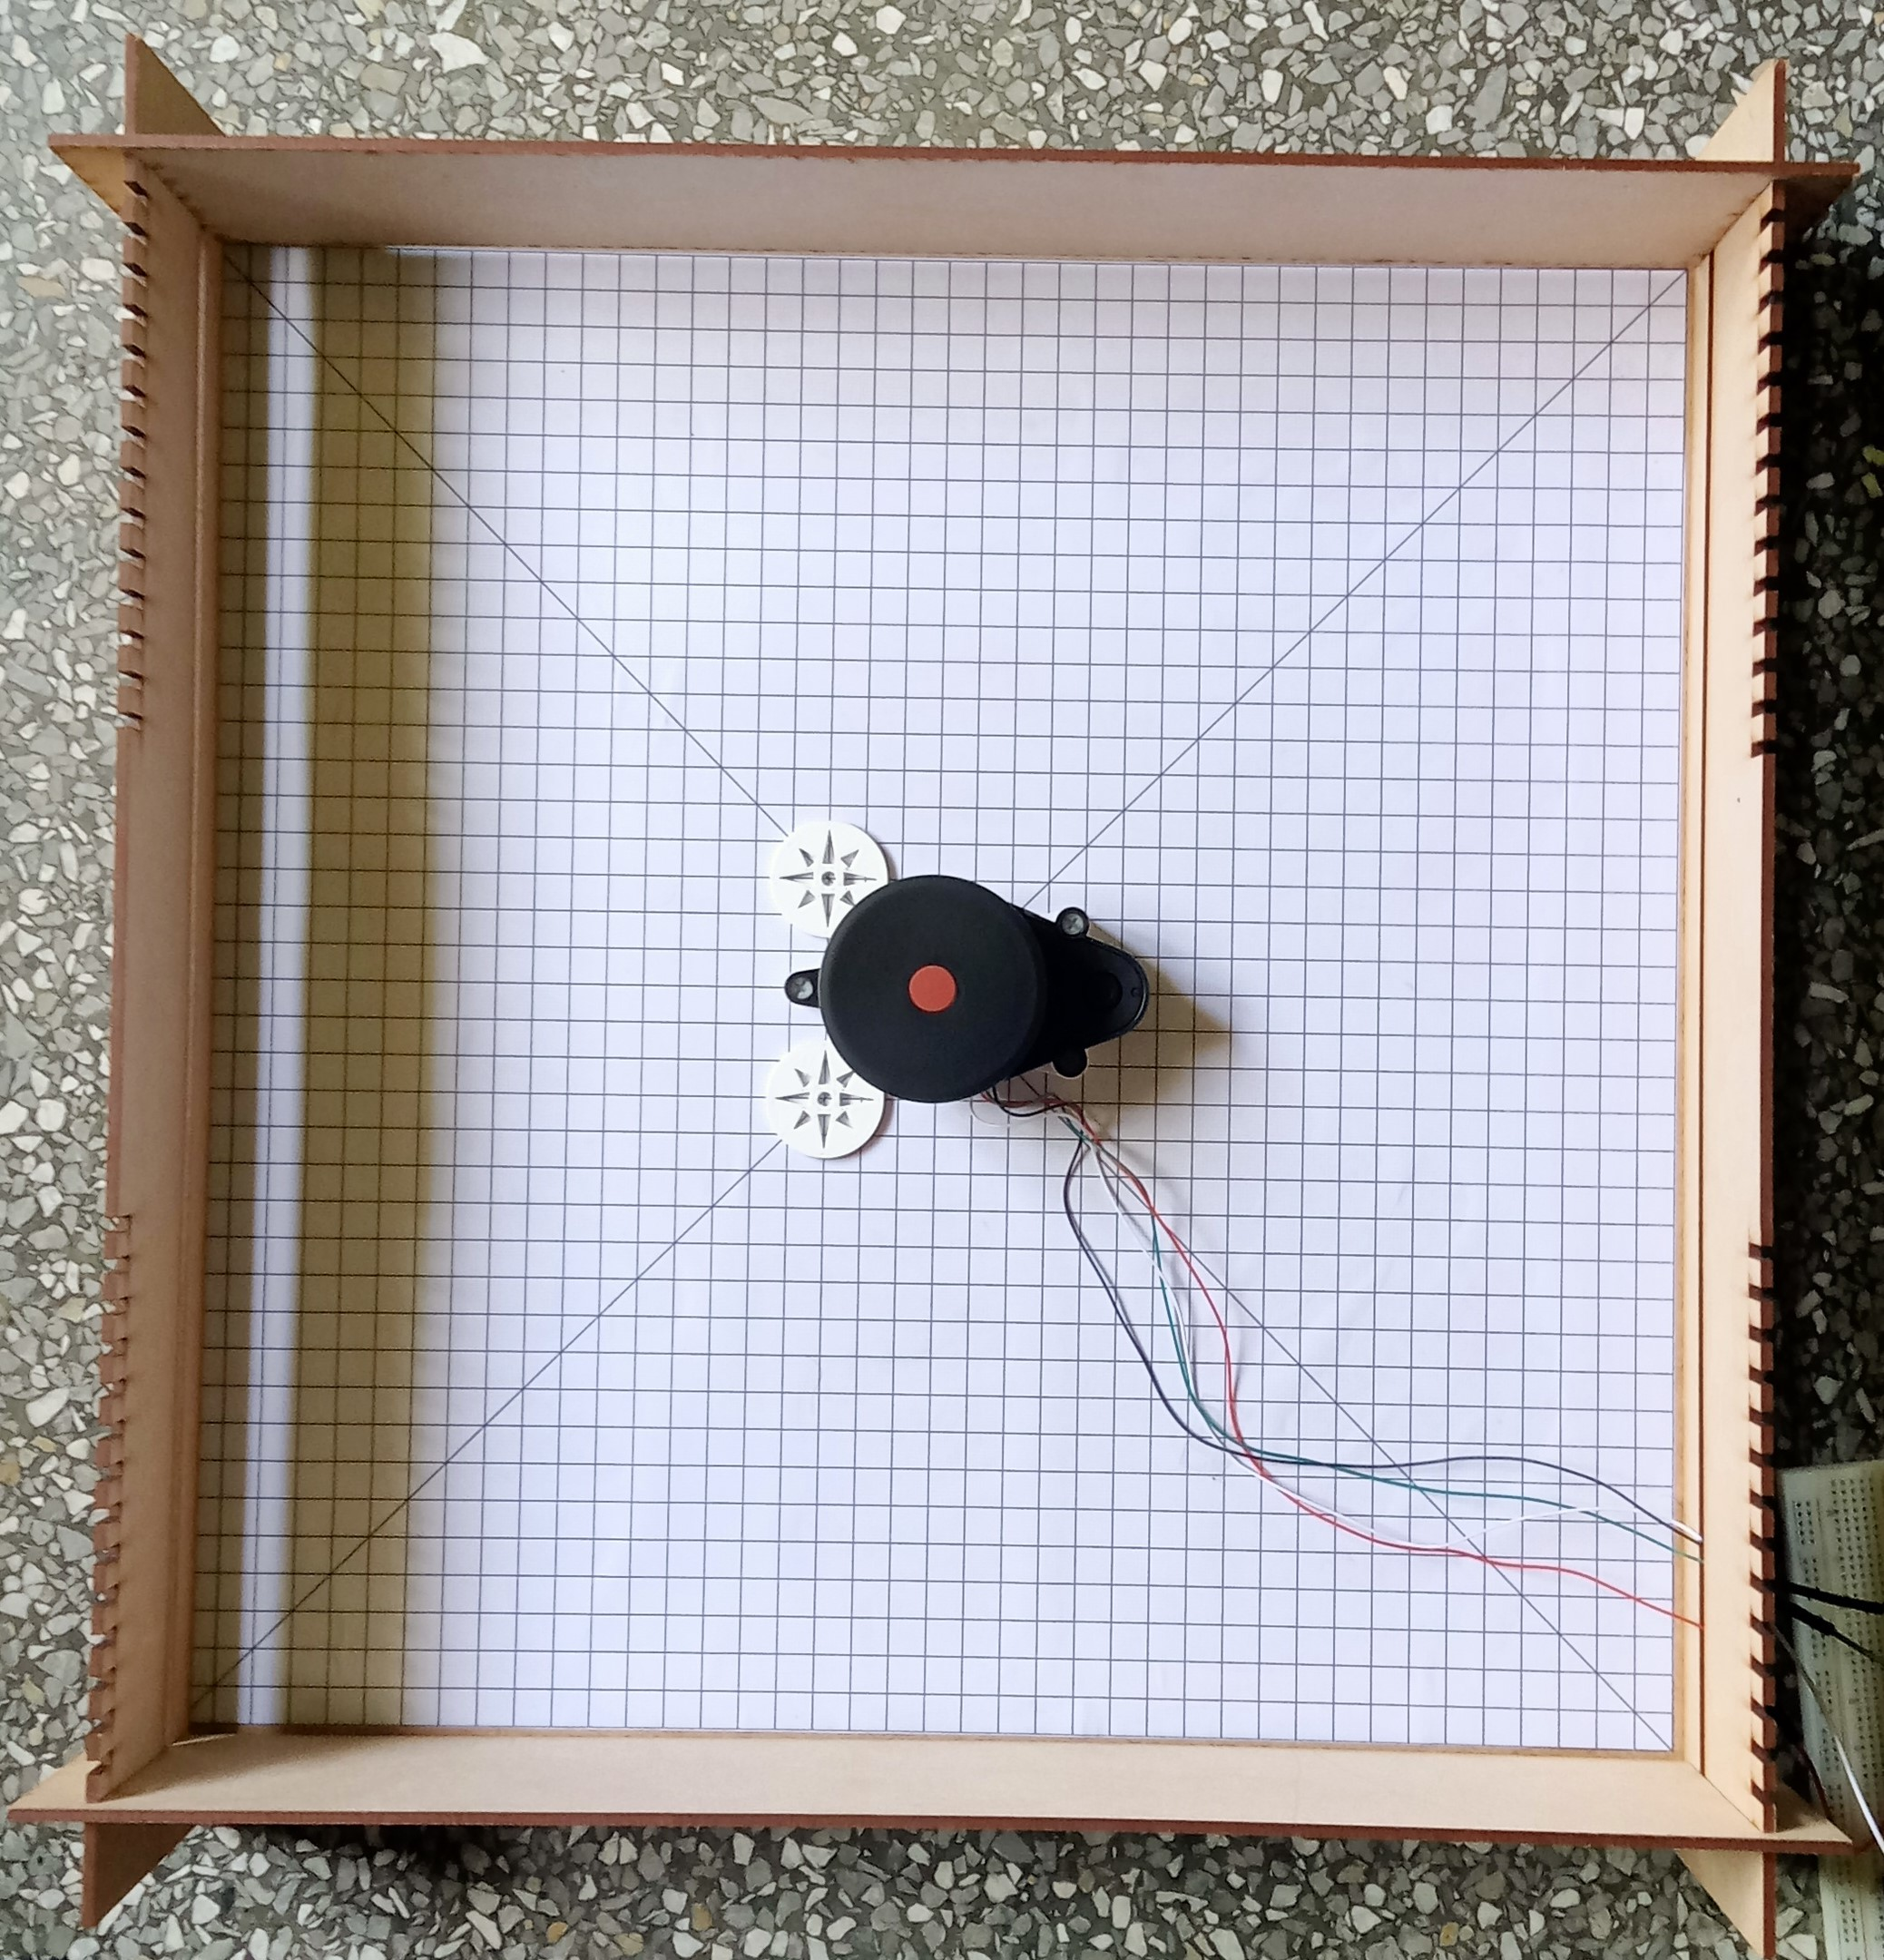
\includegraphics[width=0.5\textwidth]{plataforma.jpg}
	\caption{Vista superior de la plataforma de pruebas.}
	\label{fig:plataforma_fisica}
\end{figure}

Para asegurar una detección eficiente y minimizar el ruido generado por componentes estructurales de los agentes robóticos donde se instalará el sensor, se definió un rango mínimo de operación de 15 cm. Considerando un robot móvil como el Pololu 3pi+, permitir que el sensor opere a distancias menores podría hacer que registre elementos de su propia estructura, afectando negativamente la precisión de las mediciones. Además, dado que es poco probable encontrar obstáculos relevantes a menos de 15 cm, este límite permite enfocar la detección en elementos que realmente impacten la navegación y mejoren la maniobrabilidad del robot.

\section{Calibración de las mediciones del LiDAR FHL-LD20}
\label{sec:calibracion}

En la primera reconstrucción realizada (Figura \ref{primera_corrida}), se observaron deformaciones en las aristas de la caja, que no coincidían con los bordes rectos de la caja física. Estas deformaciones fueron causadas por la falta de corrección angular debida al desplazamiento físico del emisor/receptor del láser dentro de la carcasa. Este desplazamiento implica que el punto exacto desde donde se emite el láser y donde el sensor recoge las reflexiones está ligeramente descentrado con respecto al eje de rotación del sensor.

Cuando el láser no se emite desde el centro del círculo ideal que describe el barrido del LiDAR, se produce un desfase que afecta la precisión angular. Sin embargo, este desplazamiento interno no afecta la distancia medida, ya que sigue siendo una medición directa entre el sensor y el objeto. La luz viaja y vuelve directamente, similar a cómo se usaría una regla para medir la distancia en línea recta. El problema radica en que, un desfase angular interno provoca que el punto aparezca en una ubicación incorrecta en el plano, es decir, más a la izquierda o derecha de su verdadera posición.

El giro del sensor sobre un eje para medir diferentes ángulos genera inconsistencias cuando el emisor/receptor del láser está desplazado del centro de rotación. En este caso, los ángulos registrados no representan con precisión la posición real de los objetos en el entorno. Para abordar este error, la documentación del fabricante sugiere realizar una corrección basada en el código fuente proporcionado \cite{youyeetoo_tech_ld20_nodate}. En este proceso, se utilizan dos valores ajustados:  ``x\_val'' y ``y\_val'', que incorporan los desplazamientos físicos del emisor/receptor en los ejes X y Y. Estos valores no representan las coordenadas cartesianas de los puntos medidos, sino que funcionan como parámetros de ajuste para calcular y corregir el error angular causado por el desfase interno del sensor.

\begin{center}
	\begin{equation}
		\label{eq:valor_ajustado_x}
		\begin{array}{c}
			x\_val = distancia\_radial + x\_offset \\
			\text{donde:} \\
			x\_offset = 5.9
		\end{array}
	\end{equation}
\end{center}

\begin{center}
	\begin{equation}
		\label{eq:valor_ajustado_y}
		\begin{array}{c}
			x\_val = distancia\_radial \times y\_factor + y\_offset \\
			\text{donde:} \\
			y\_offset = -18.975571 \\
			y\_factor = 0.11923
		\end{array}
	\end{equation}
\end{center}

En la Ecuación \ref{eq:valor_ajustado_y}, el valor ajustado ``y\_val'' utiliza una constante  ``y\_factor'' de 0.11923. Aunque la documentación no especifica la razón exacta de este valor, se puede inferir que su propósito era corregir la proyección angular de las mediciones. Probablemente compensando una inclinación natural del sensor o representando un ajuste empírico destinado a mejorar la precisión de las mediciones. A partir de los valores ajustados, se calcula un ángulo de corrección usando la función arcotangente de la relación ``y\_val'' sobre ``x\_val''. Este ángulo de corrección refleja cuánto debe sumarse o restarse al ángulo original para compensar el desplazamiento interno del sensor. 

Si el sistema utiliza coordenadas en sentido antihorario, el angulo se invierte (restándole 360 grados) y luego se suma el ángulo de corrección para obtener el valor final. En caso contrario, el ángulo de corrección se resta directamente del ángulo original. La Figura \ref{fig: comparación_con_sin_corre}, muestra la disposición del sensor dentro de la caja, junto con una comparación de la reconstrucción visual obtenida a partir de tres revoluciones completas capturadas, utilizando el ángulo sin y con corrección.

\begin{figure}[H]
	\centering
	\begin{subfigure}{0.6\textwidth}
		\centering
		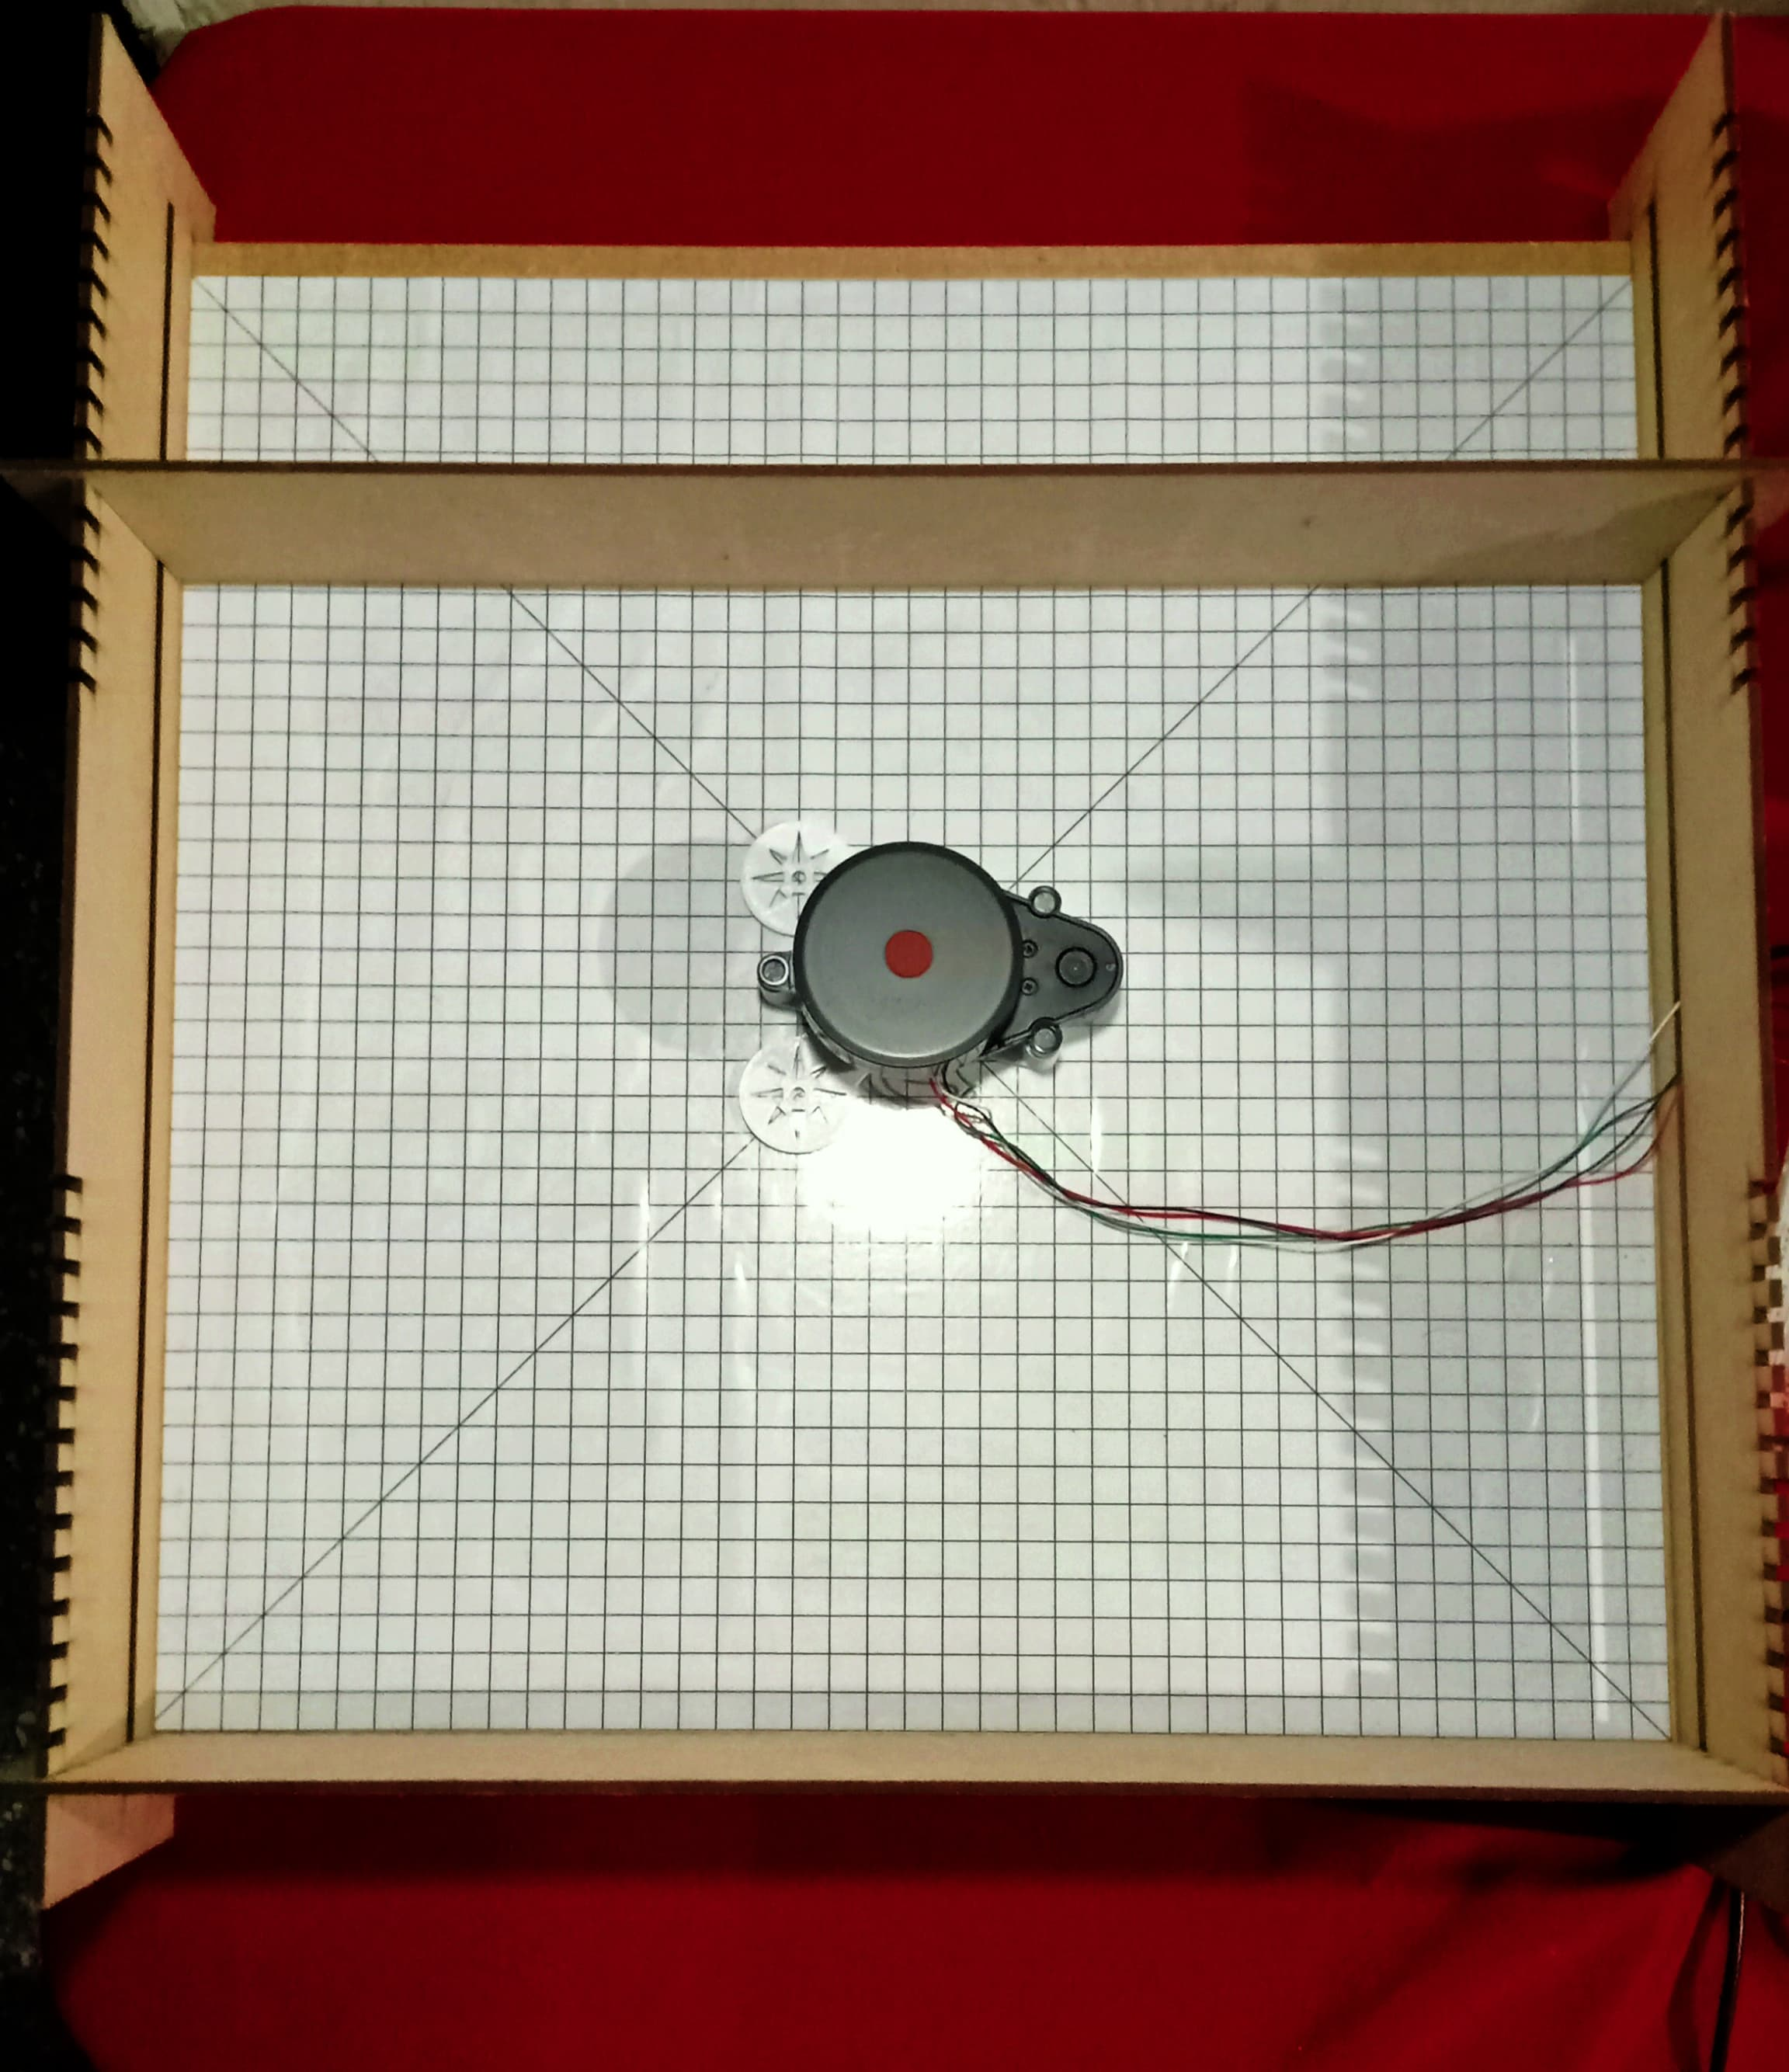
\includegraphics[width=0.6\linewidth]{disposicion_lidar2.jpeg}
		\caption{Disposición del sensor FHL-LD20 dentro de la caja}
		\label{disposicion_lidar2}
		\vspace{1em}
	\end{subfigure}
	\begin{subfigure}{0.45\textwidth}
		\centering
		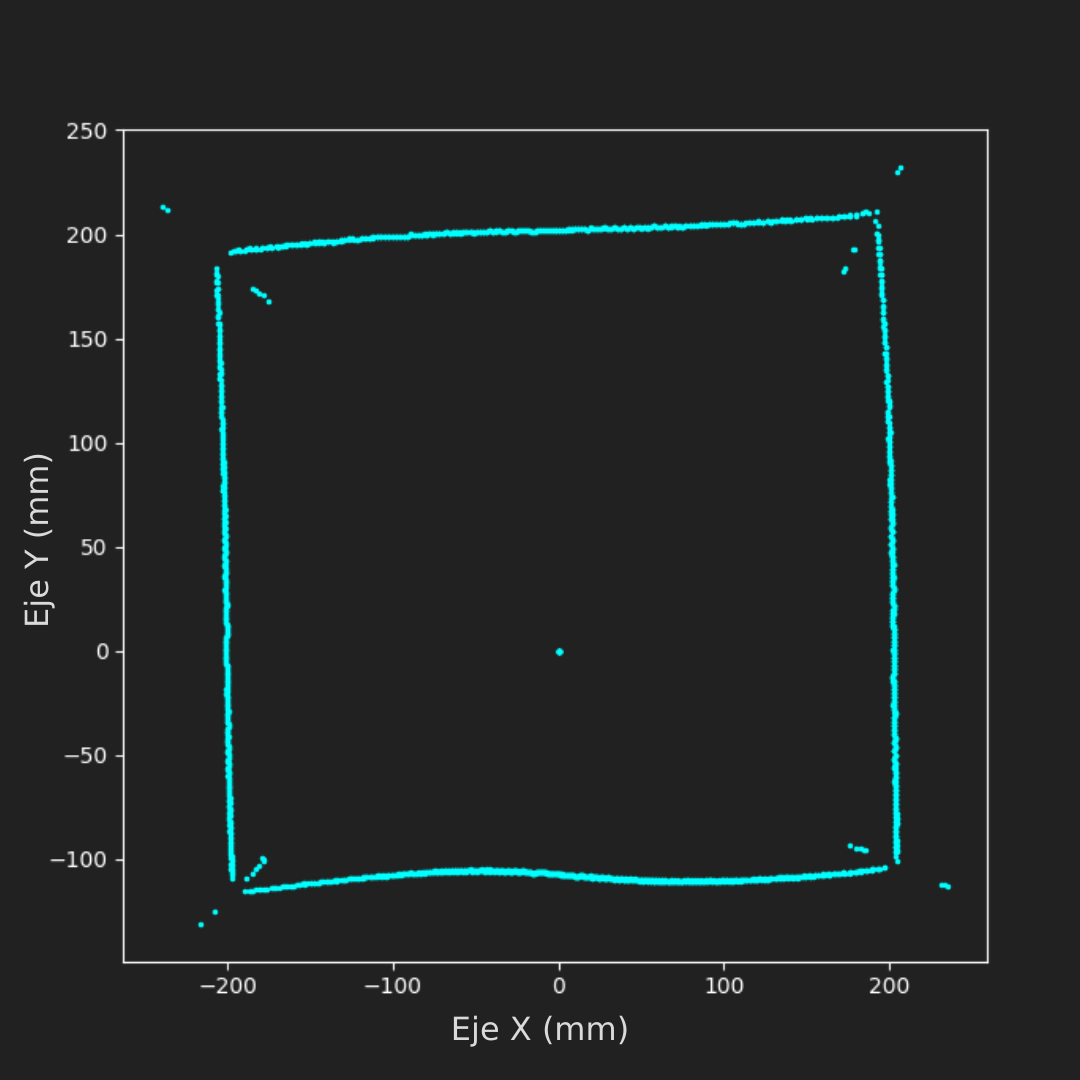
\includegraphics[width=0.9\linewidth]{lectura_sin_corre.png}
		\caption{Reconstrucción de tres revoluciones completas capturadas sin ángulo de corrección}
		\label{lectura_sin_corre}
	\end{subfigure}
	\hspace{1em}
	\begin{subfigure}{0.45\textwidth}
		\centering
		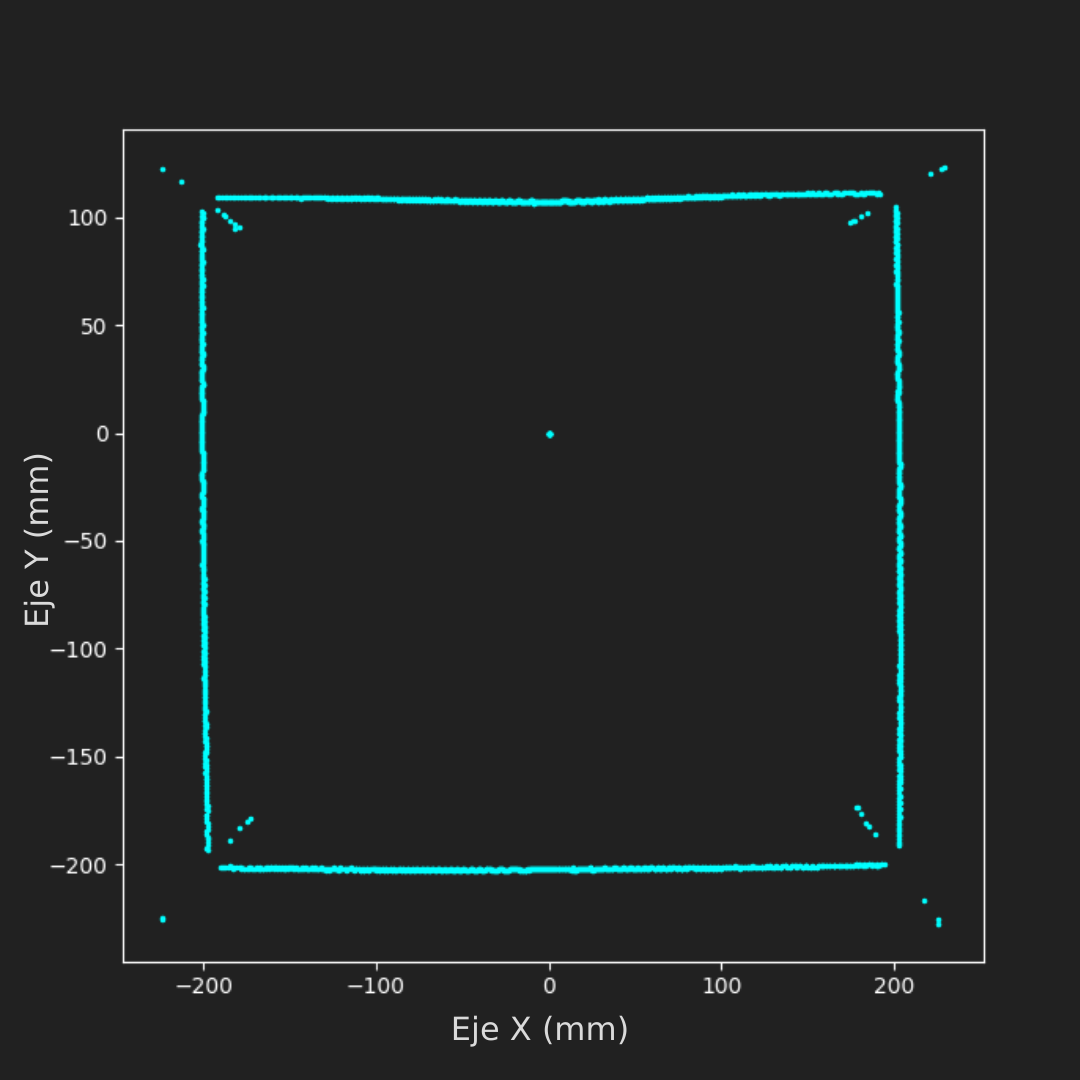
\includegraphics[width=0.9\linewidth]{lectura_con_corre.png}
		\caption{Reconstrucción de tres revoluciones completas capturadas con ángulo de corrección}
		\label{lectura_con_corre}
	\end{subfigure}
	\caption{Comparación de la reconstrucción con y sin ángulo de corrección: tres revoluciones completas capturadas.}
	\label{fig: comparación_con_sin_corre}
\end{figure}

\section{Precisión del LiDAR FHL-LD20 después del proceso de calibración}
Para verificar la calibración del sensor, se colocó en el centro de la plataforma utilizando las brújulas incluidas en el soporte para asegurar su alineación. Una vez posicionado, se realizó una captura de tres revoluciones completas y se compararon los valores medidos de las aristas con los valores nominales esperados. Se realizó un análisis de la reconstrucción obtenida empleando como escenario la plataforma de pruebas preliminares. Este análisis incluyó la determinación de regresiones lineales en las aristas detectadas y el cálculo de diversas métricas para medir la fidelidad de las mediciones realizadas por el sensor. El proceso para evaluar la precisión del sensor para una caja de 400 $\times$ 400 mm se detalla a continuación.

En primer lugar, se aplicó un filtro para seleccionar los puntos más cercanos a las aristas esperadas, utilizando un intervalo de tolerancia de $\pm$ 5 mm.  Luego, se excluyó una franja de 8 mm alrededor de los bordes de la caja para minimizar distorsiones relacionadas con el efecto de las esquinas, donde el ángulo de incidencia del haz sobre la superficie dificulta la detección precisa de la geometría. Estas áreas generan reflexiones difusas que alteran las mediciones del sensor (ver Sección \ref{mediciones_angulares}).  Tras el filtrado, se procedió a obtener la regresión lineal para cada conjunto de puntos que definía una arista de la caja reconstruida. Como se muestra en las Figuras \ref{fig: reconstruccion_analisis_horizontal_1}, las aristas horizontales se ajustaron los valores del eje Y en función de los del eje X, mientras que para las aristas verticales se invirtió esta relación, ajustando los valores del eje X en función de los del eje Y (ver Figura \ref{fig: reconstruccion_analisis_vertical_1}). Este procedimiento evitó pendientes tendientes a infinito en las aristas verticales, generando pendientes cercanas a cero que facilitan su interpretación. De este modo, se logró una representación más clara y consistente de las características geométricas de la caja reconstruida.

A partir de los puntos filtrados y las regresiones obtenidas, se calcularon las siguientes métricas para cada arista:
\begin{itemize}
	\item Ecuación de la recta: Pendiente e intercepto obtenidos a partir del ajuste lineal.
	\item Intervalos de confianza (IC): Para la pendiente e intercepto, se calcularon intervalos de confianza del 95\%, proporcionando una medida de la incertidumbre en la estimación de los parámetros de la recta.
	\item Diferencia promedio. Media de las diferencias entre los puntos detectados y el valor real esperado, proporcionando una medida del error sistemático del sensor.
	\item Medición máxima y mínima: Los valores extremos detectados en cada conjunto de puntos que indican la variabilidad en las mediciones.
	\item Rango: Diferencia entre el valor máximo y mínimo, lo que refleja la dispersión de las mediciones.
\end{itemize}

Para evaluar la rectitud de las aristas, se analizaron las pendientes obtenidas a partir del ajuste lineal. Los valores obtenidos muestran desviaciones mínimas respecto a la horizontalidad o verticalidad ideal, evidenciando una inclinación prácticamente despreciable. Por ejemplo, la pendiente máxima observada para las aristas horizontales fue de 0.0073 (ver Figura \ref{analisis_precision_1_3}), lo que corresponde a un ángulo de inclinación aproximado de 0.42° respecto al eje horizontal, mientras que la máxima para las aristas verticales fue de 0.0077, con un ángulo de inclinación de 0.44° respecto al eje vertical (ver Figura \ref{analisis_precision_1_4}). Estas inclinaciones son insignificantes en comparación con la escala de la plataforma (400 $\times$ 400 mm) y se encuentran dentro de los márgenes atribuibles a errores en las herramientas de medición, así como a ligeras imprecisiones experimentales durante la orientación del sensor.

Los intervalos de confianza calculados para estas pendientes presentan rangos estrechos, reflejando una alta consistencia en las mediciones y una baja variabilidad entre los puntos analizados. Las magnitudes de las pendientes, todas cercanas a cero, corroboran que las aristas reconstruidas se aproximan con gran precisión a la geometría ideal de líneas rectas. Estos resultados demuestran que el sistema es capaz de capturar la rectitud esperada con un nivel de precisión altamente satisfactorio.

\begin{figure}[H]
	\centering
	\begin{subfigure}{\textwidth}
		\centering
		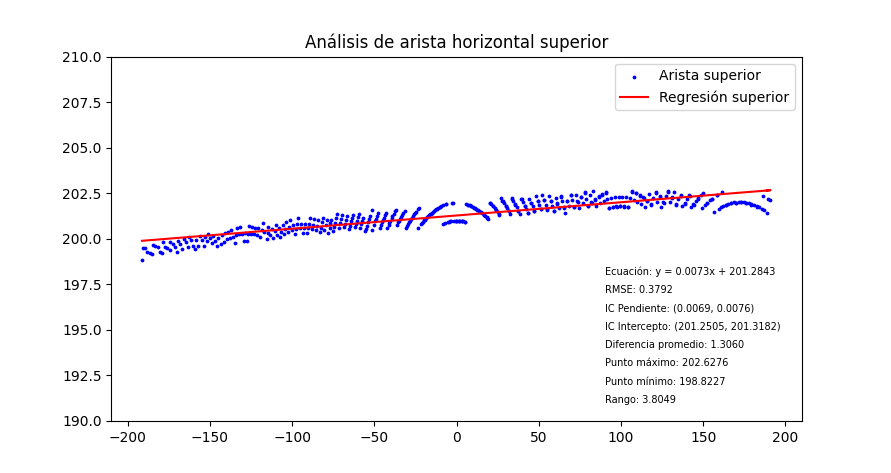
\includegraphics[width=1.5\linewidth]{analisis_precision_1_1.png}
		\caption{Análisis de arista horizontal superior}
		\label{analisis_precision_1_1}
	\end{subfigure}
	\hspace{1em}
	\begin{subfigure}{\textwidth}
		\centering
		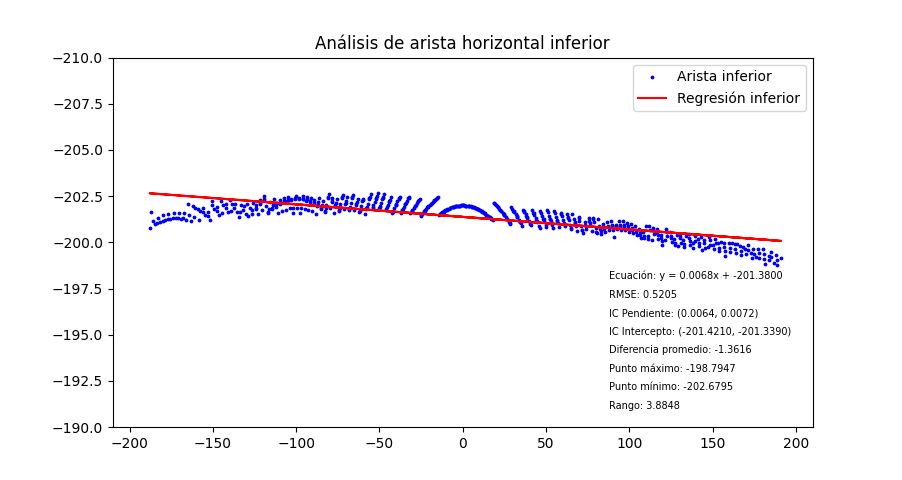
\includegraphics[width=1.5\linewidth]{analisis_precision_1_2.png}
		\caption{Análisis de arista horizontal inferior}
		\label{analisis_precision_1_2}
	\end{subfigure}
	\caption{Análisis de la reconstrucción realizada para las aristas horizontales de una caja de 400$\times$400 mm: tres revoluciones completas capturadas.}
	\label{fig: reconstruccion_analisis_horizontal_1}
\end{figure}

\begin{figure}[H]
	\centering
	\begin{subfigure}{0.45\textwidth}
		\centering
		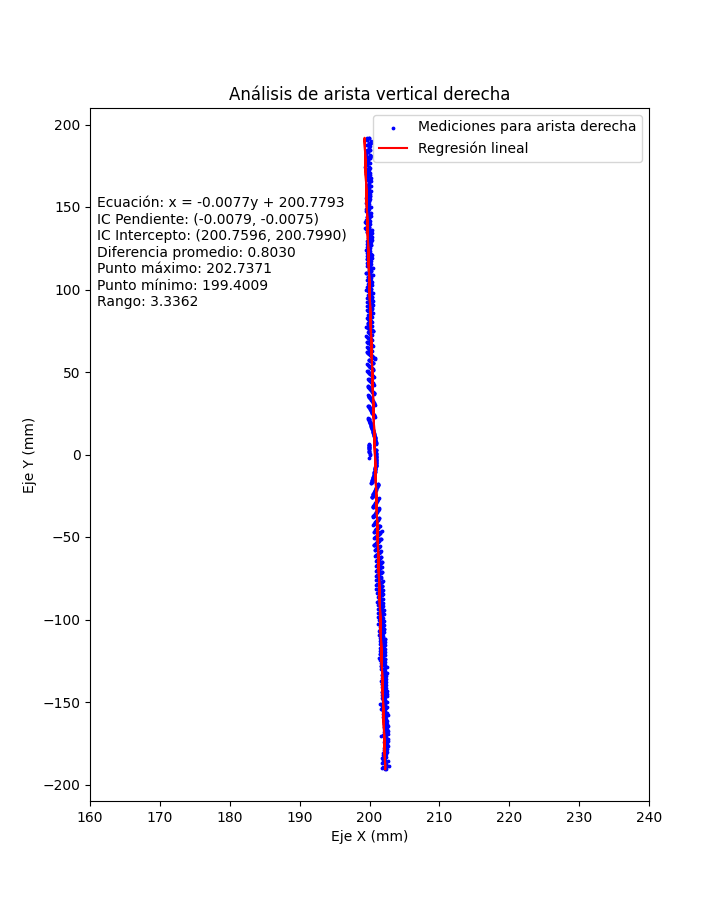
\includegraphics[width=1.2\linewidth]{analisis_precision_1_3.png}
		\caption{Análisis de arista vertical derecha}
		\label{analisis_precision_1_3}
	\end{subfigure}
	\hspace{1em}
	\begin{subfigure}{0.45\textwidth}
		\centering
		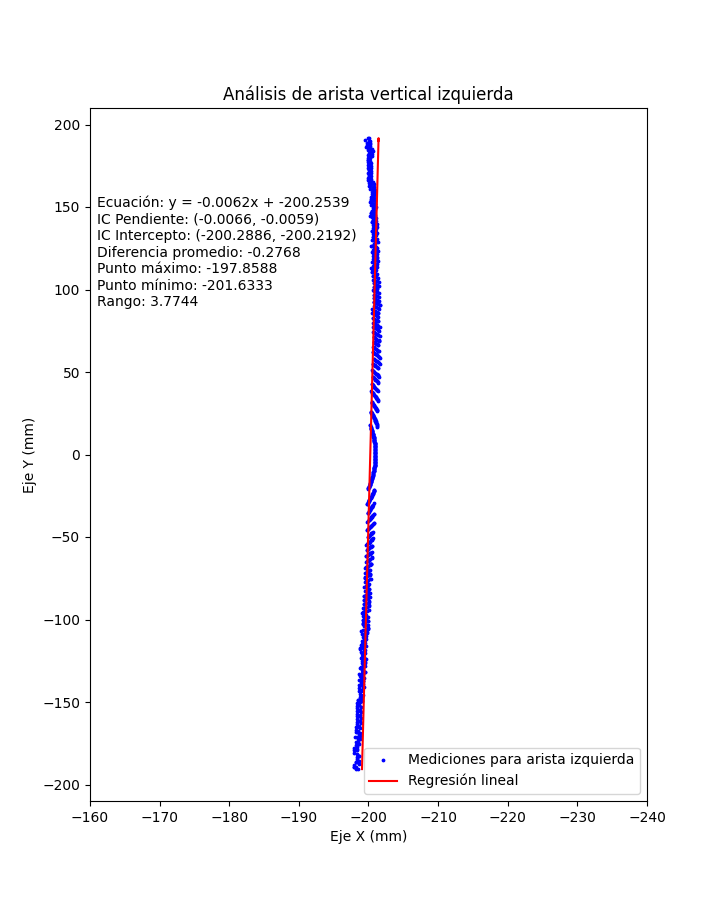
\includegraphics[width=1.2\linewidth]{analisis_precision_1_4.png}
		\caption{Análisis de arista vertical izquierda}
		\label{analisis_precision_1_4}
	\end{subfigure}
	\caption{Análisis de la reconstrucción realizada para las aristas verticales de una caja de 400$\times$400 mm: tres revoluciones completas capturadas.}
	\label{fig: reconstruccion_analisis_vertical_1}
\end{figure}

El intercepto calculado resulta útil para evaluar el alineamiento general del sensor con respecto a las posiciones esperadas. En todos los casos, se observan ligeras desviaciones en el intercepto que oscilaban entre 0.3959 mm y 2.4565 mm con respecto a las dimensiones esperadas de $\pm$ 200 mm, lo cual es relativamente bajo. El análisis de los intervalos de confianza de la pendiente y el intercepto proporciona una medida de la fiabilidad de estos parámetros. Al mostrar rangos estrechos, se demuestra una fuerte consistencia en las mediciones, lo cual refuerza la confiabilidad de las regresiones lineales obtenidas. 

El rango de las mediciones, que varió entre 3.8049 mm y 4.4322 mm para las diferentes aristas, refleja una dispersión controlada. La diferencia promedio entre las mediciones registradas y el valor real esperado, inferior a 3 mm, confirma que la dispersión de las mediciones se encuentra dentro de los límites de precisión indicados en la Sección \ref{var_dist}. En resumen, las métricas analizadas demuestran que el sensor presenta una buena precisión general. A pesar que se observen pequeñas desviaciones, los errores están por debajo de los 5 mm, lo cual es aceptable para la mayoría de las aplicaciones, en especial para navegación autónoma.

En la Sección \ref{caracterizacion} se detallan pruebas adicionales que complementan el proceso de calibración, proporcionando información clave para el posprocesamiento de los datos. Estas pruebas permiten analizar en mayor profundidad la precisión y consistencia del sensor en diferentes escenarios, lo que resulta esencial para su correcta calibración posprocesamiento. A partir de los resultados descritos en los párrafos anteriores y de las pruebas realizadas en la siguiente sección, se definieron los criterios de evaluación para la calibración del sensor:

\begin{itemize}
	\item Exactitud al reconstruir las dimensiones de objetos calibrados (escenarios circulares o plataforma de pruebas): Los valores reconstruidos deben coincidir con las dimensiones nominales de referencia, con desviaciones menores a $\pm$ 5 mm.
	\item Diferencia entre la distancia medida y la distancia real: El error promedio debe mantenerse por debajo de 3 mm, conforme a los límites de precisión indicados en la Sección \ref{caracterizacion}.
	\item Variabilidad en las mediciones realizadas en condiciones idénticas: La dispersión debe ser mínima, con un rango de variabilidad inferior a $\pm$ 5 mm en mediciones repetidas en las mismas condiciones.
	\item Consistencia de las pendientes en las aristas reconstruidas: Para el caso de escenarios cuadrados/rectangulares, al centrar correctamente el LiDAR utilizando su soporte, las pendientes obtenidas de las regresiones deben ser cercanas a cero, reflejando la rectitud esperada de la geometría.
	\item Análisis de la dispersión angular en puntos de transición geométrica: Los valores mínimos, máximos y promedio de las mediciones angulares deben alinearse con los valores teóricos esperados, con una variabilidad inferior a $\pm$ 3° (ver Sección\ref{mediciones_angulares}).
\end{itemize}

Estos criterios resultan relevantes para evaluar la capacidad del sensor en escenarios que abarcan tanto geometrías simples como aquellas con transiciones abruptas. Cabe señalar que la variabilidad en las mediciones indicadas en los criterios, con márgenes de ±3 mm, ±5 mm o ±3°, son prácticamente despreciables en la aplicación de navegación autónoma dentro de un espacio de trabajo como lo puede ser el Robotat (4.8$\times$3.8 m) o en el rango mínimo de medición establecido de 15 cm (ver Sección \ref{minima_dist}). Sin embargo, se recomienda implementar técnicas de posprocesamiento, como el suavizado de datos o algoritmos de compensación geométrica, para mitigar las dispersiones en las mediciones. Dichas técnicas deben considerar la variabilidad identificada en esta y la siguiente sección, tanto para las mediciones radiales como para las angulares, permitiendo así compensar o mitigar dicha variabilidad y generando mejores aproximaciones del entorno.

\chapter{Caracterización del LiDAR FHL-LD20}
\label{caracterizacion}
En este capítulo se describe la caracterización del sensor LiDAR FHL-LD20, un procedimiento diseñado para evaluar y modelar la confiabilidad de sus mediciones bajo condiciones reales de operación. Este análisis se centra en las variaciones presentes en las mediciones de distancia y ángulo registradas por el sensor. Proporciona, además, una comprensión detallada de los parámetros de incertidumbre asociados, los cuales facilitan su integración en algoritmos de percepción y navegación autónoma, como el filtro de Kalman extendido (EKF). Este proceso permite validar las especificaciones proporcionadas por el fabricante, que pueden diferir del desempeño real en campo. Además, resulta clave para adaptar el sensor a las condiciones específicas de la aplicación, identificar posibles limitaciones y optimizar su configuración para maximizar su rendimiento en la implementación final.

\section{Depuración de mediciones nulas en el LiDAR FHL-LD20}
Como se describe en la Sección \ref{sec:calibracion}, el proceso de calibración utiliza las distancias en formato decimal, para calcular el ángulo de corrección, el cual ajusta la posición angular de los puntos medidos por el LiDAR. En el diagrama de flujo (Figura \ref{fig:diagrama_procesamiento_dec}), se puede apreciar que el procesamiento depende de si la distancia medida es mayor a cero. Cuando es mayor, se calculan tanto los valores de ajuste como el ángulo de desplazamiento real. Una vez determinado el ángulo real, se actualiza el valor del ángulo de corrección antiguo por el más reciente.

\begin{figure}[H]
	\centering
	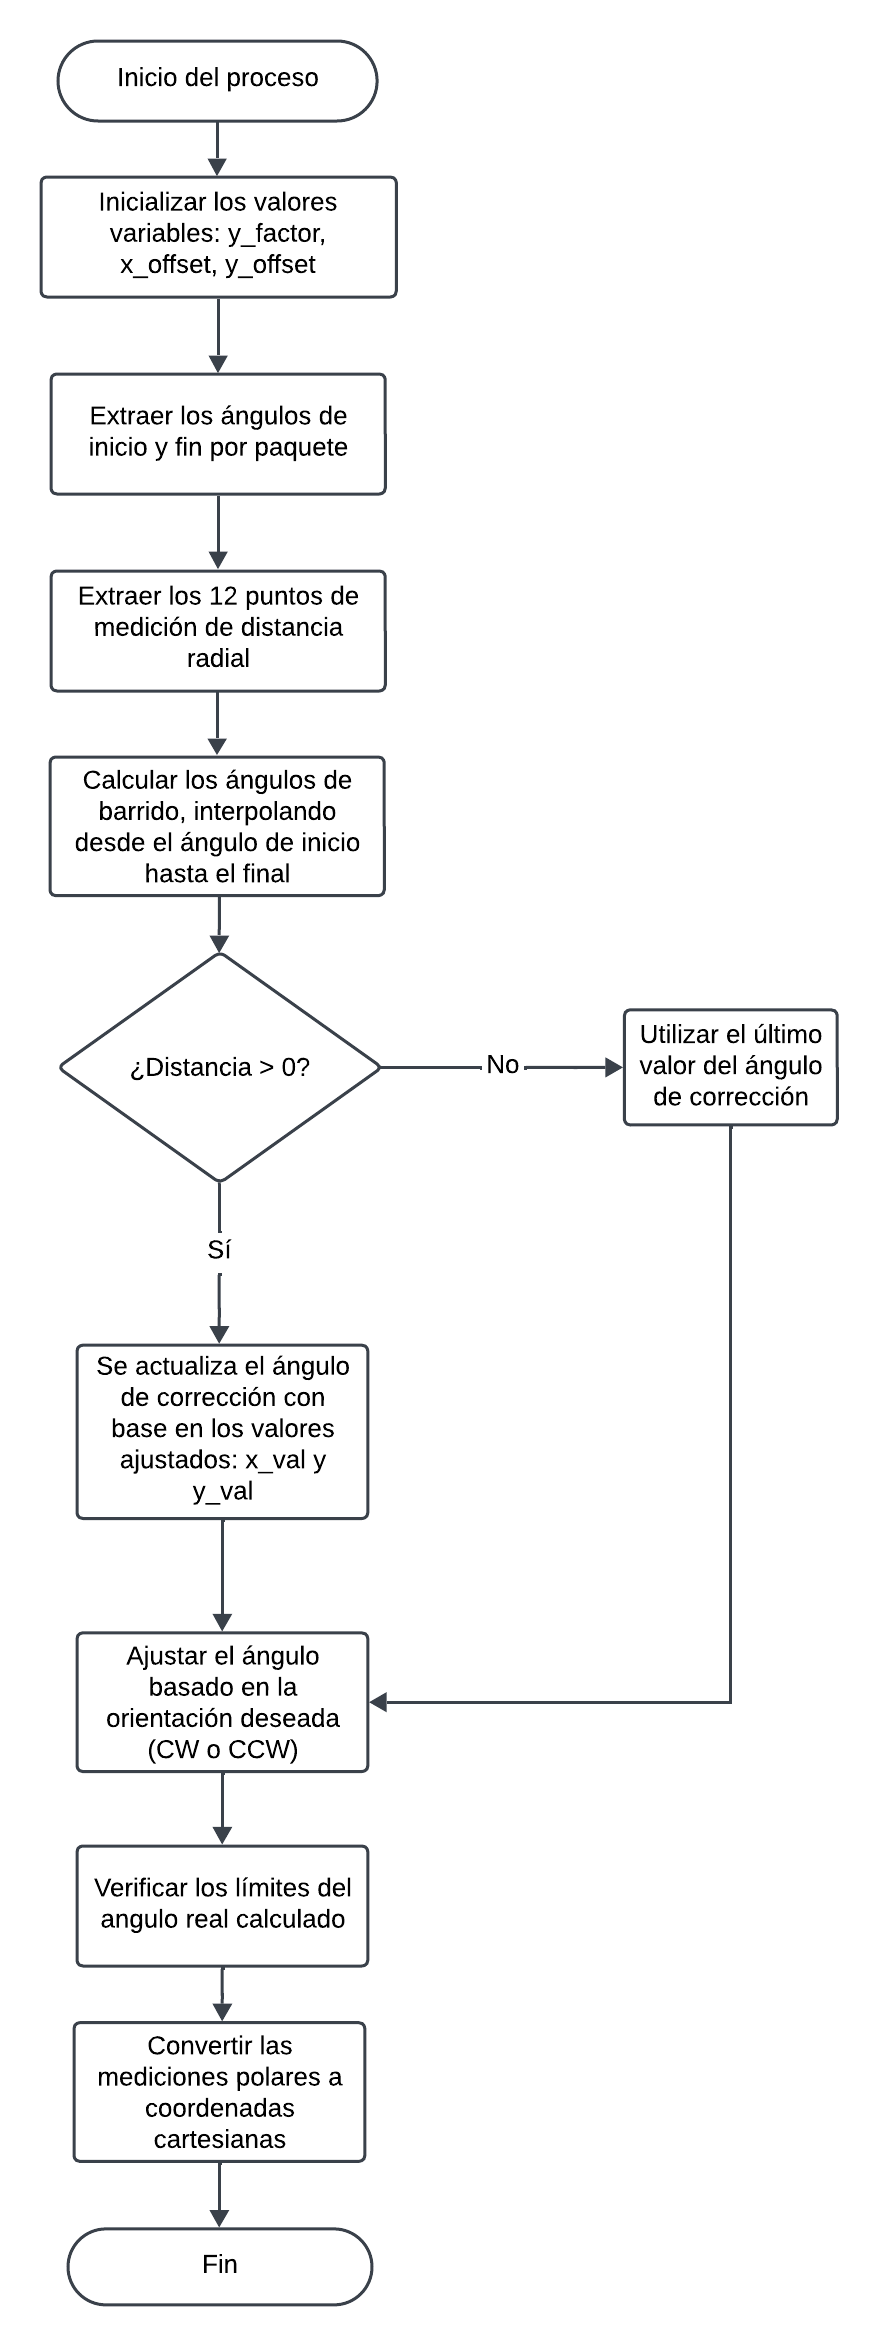
\includegraphics[width=0.4\textwidth]{diagrama_procesamiento_dec.png}
	\caption{Diagrama de flujo general para procesamiento de datos en formato decimal.}
	\label{fig:diagrama_procesamiento_dec}
\end{figure}

En caso de que la distancia medida sea igual a cero, no se recalculan los valores de ajuste, ya que la medición carece de información para ese punto. En su lugar, se reutiliza el último ángulo de corrección calculado, para ajustar el ángulo real de esa medición nula. Este procedimiento garantiza que incluso estas mediciones mantengan una continuidad angular coherente respecto a las anteriores, evitando distorsiones en la reconstrucción del entorno. Sin embargo, incluir estas mediciones nulas en los gráficos de coordenadas polares y cartesianas resulta innecesario, ya que, físicamente, el sensor no es capaz de registrar mediciones justo en su eje de rotación. 

Estos puntos añaden cierta confusión visual al interpretar el entorno capturado. Por esta razón, se optó por filtrar las mediciones cuya distancia radial fuese cero. Al eliminar estos puntos en la generación de los gráficos, se preservan solo las distancias que aportan información relevante sobre el entorno. Este filtrado mejora la claridad y precisión de la representación de los objetos detectados, lo cual mejora la interpretación de los datos capturados. En la Figura \ref{fig: comparación_con_sin_filt} se muestra la comparación antes y después de depurar las mediciones nulas capturadas.

\begin{figure}[H]
	\centering
	\begin{subfigure}{0.6\textwidth}
		\centering
		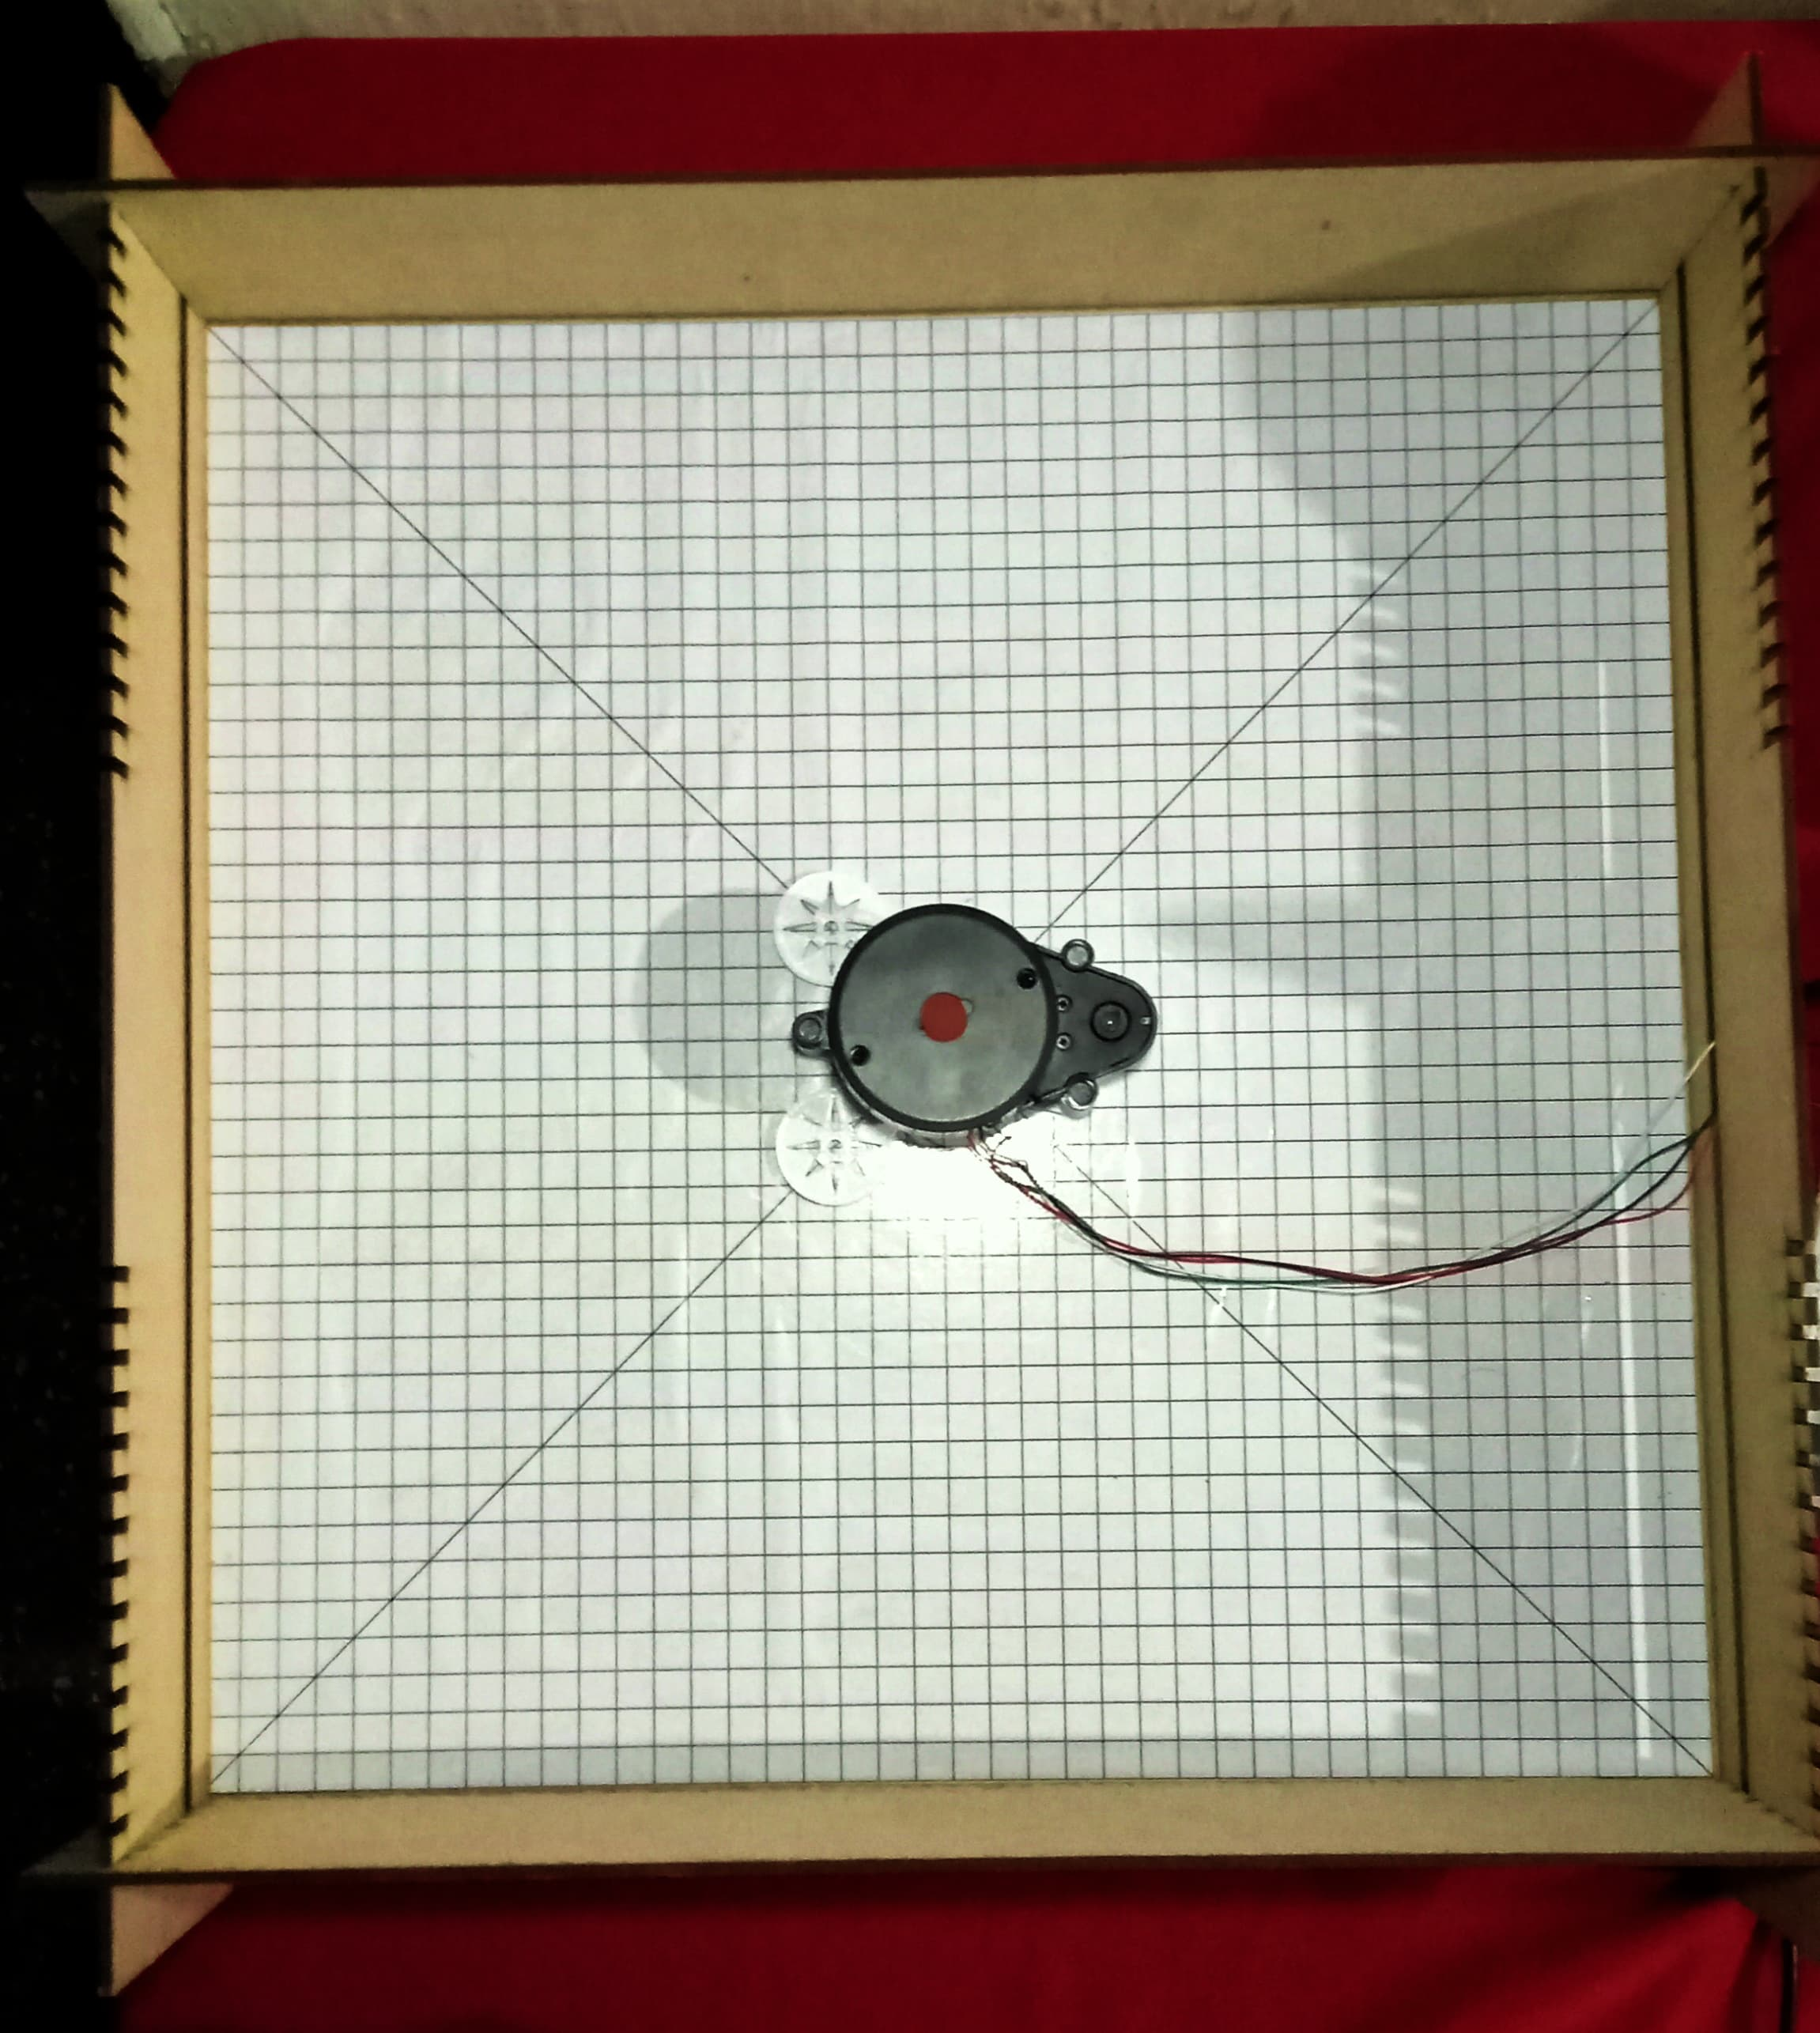
\includegraphics[width=0.7\linewidth]{disposicion_lidar3.jpeg}
		\caption{Disposición del sensor FHL-LD20 dentro de la caja.}
		\label{disposicion_lidar3}
		\vspace{1em}
	\end{subfigure}
	\begin{subfigure}{0.45\textwidth}
		\centering
		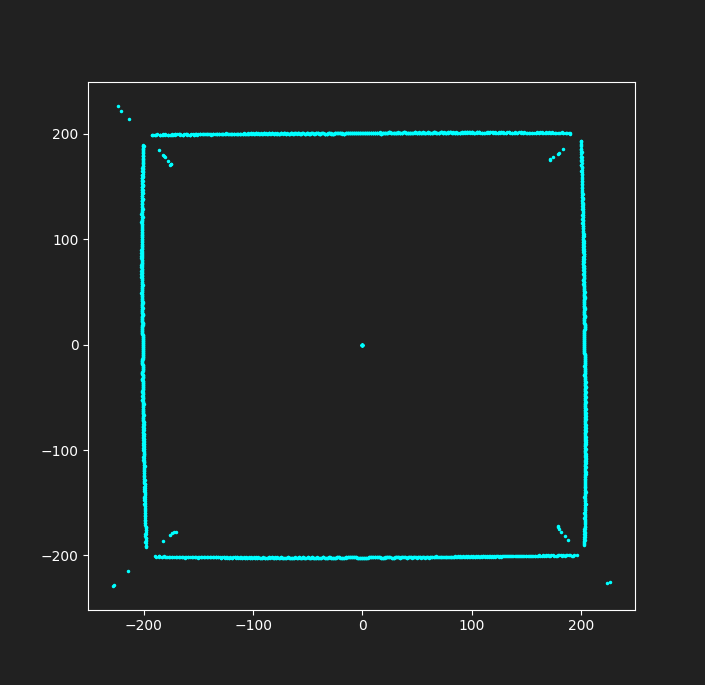
\includegraphics[width=0.9\linewidth]{lectura_sin_filt.png}
		\caption{Reconstrucción de tres revoluciones completas capturadas sin filtro de mediciones nulas.}
		\label{lectura_sin_filt}
	\end{subfigure}
	\hspace{1em}
	\begin{subfigure}{0.45\textwidth}
		\centering
		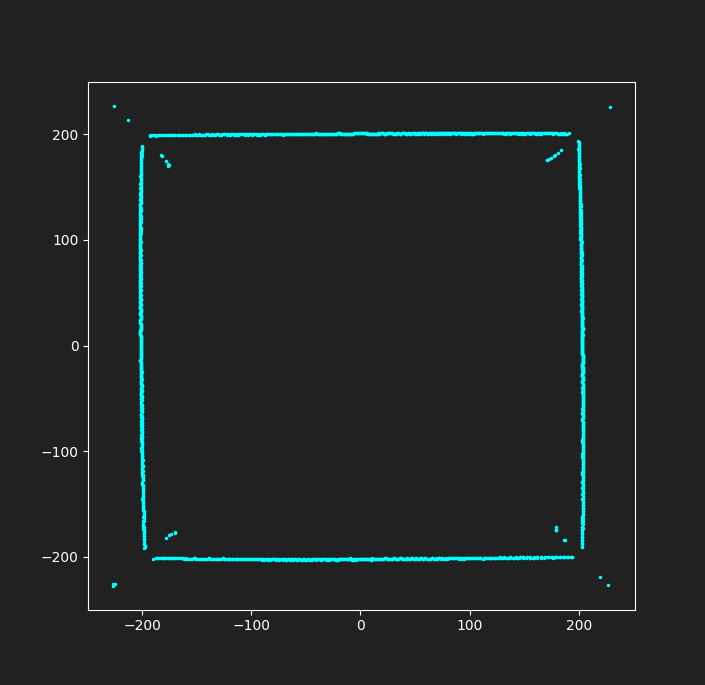
\includegraphics[width=0.9\linewidth]{lectura_con_filt.png}
		\caption{Reconstrucción de tres revoluciones completas capturadas con filtro de mediciones nulas.}
		\label{lectura_con_filt}
	\end{subfigure}
	\caption{Comparación de la reconstrucción con y sin filtro de mediciones nulas: tres revoluciones completas capturadas.}
	\label{fig: comparación_con_sin_filt}
\end{figure}

\section{Rango de medición efectivo del LiDAR FHL-LD20}
\label{minima_dist}
Determinar el rango de medición efectivo implica evaluar la distancia mínima a la que el sensor puede operar con precisión y confiabilidad. El rango mínimo de medición es fundamental para identificar las limitaciones del sensor en rangos cercanos y definir el alcance mínimo que el sensor puede capturar. Conocer este límite permite ajustar la caracterización del sensor para satisfacer las necesidades específicas de la aplicación en la que se utilizará.

\subsection{Rango mínimo de medición}
Para evaluar la distancia mínima que el sensor es capaz de medir, se diseñaron entornos circulares con diámetros cercanos a la distancia mínima especificada por el fabricante. Se imprimieron en 3D círculos de 60, 70, 80, 90 y 100 mm de radio con el fin de identificar el rango mínimo que permitiera un funcionamiento adecuado del sensor. Optar por un contorno circular en lugar de uno cuadrado resultó ventajoso, ya que la naturaleza del sensor favorece una cobertura uniforme en todas las direcciones.

En la Figura \ref{fig: reconstrucciones_vacías_6} se muestra la primera prueba, realizada con un contorno circular de 6 cm de radio. Como se aprecia en las Figuras \ref{try_6cm_r} y \ref{try_6cm_r_car}, el contorno no pudo ser reconstruido, y las gráficas resultaron vacías. Al analizar los datos sin procesar de este experimento, se descubrió que el sensor no era capaz de registrar distancias válidas, por lo que se registraban como cero (ver Figura \ref{fig:data_null}). Y, debido a que las mediciones se filtraban para eliminar las distancias nulas, la reconstrucción de los datos resultó vacía. 

Es importante señalar que, a pesar de la ausencia de mediciones de distancia válidas, el sensor aún capturaba los ángulos de inicio y final, como se muestra en la Figura \ref{fig:data_null}. Esto sugiere que la cobertura del campo de visión del sensor es independiente de su capacidad para registrar distancias radiales válidas.
\begin{figure}[H]
	\centering
	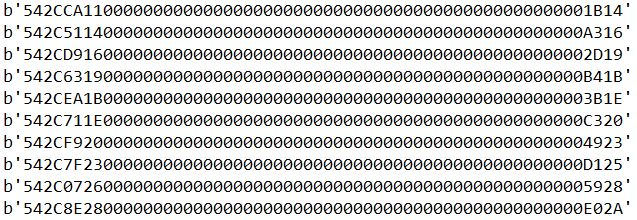
\includegraphics[width=0.8\textwidth]{lecturas_nula.jpg}
	\caption{Ejemplificación de las lecturas nulas durante la reconstrucción de mediciones: entorno circular de 60 mm de radio.}
	\label{fig:data_null}
\end{figure}

\begin{figure}[H]
	\centering
	\begin{subfigure}{0.6\textwidth}
		\centering
		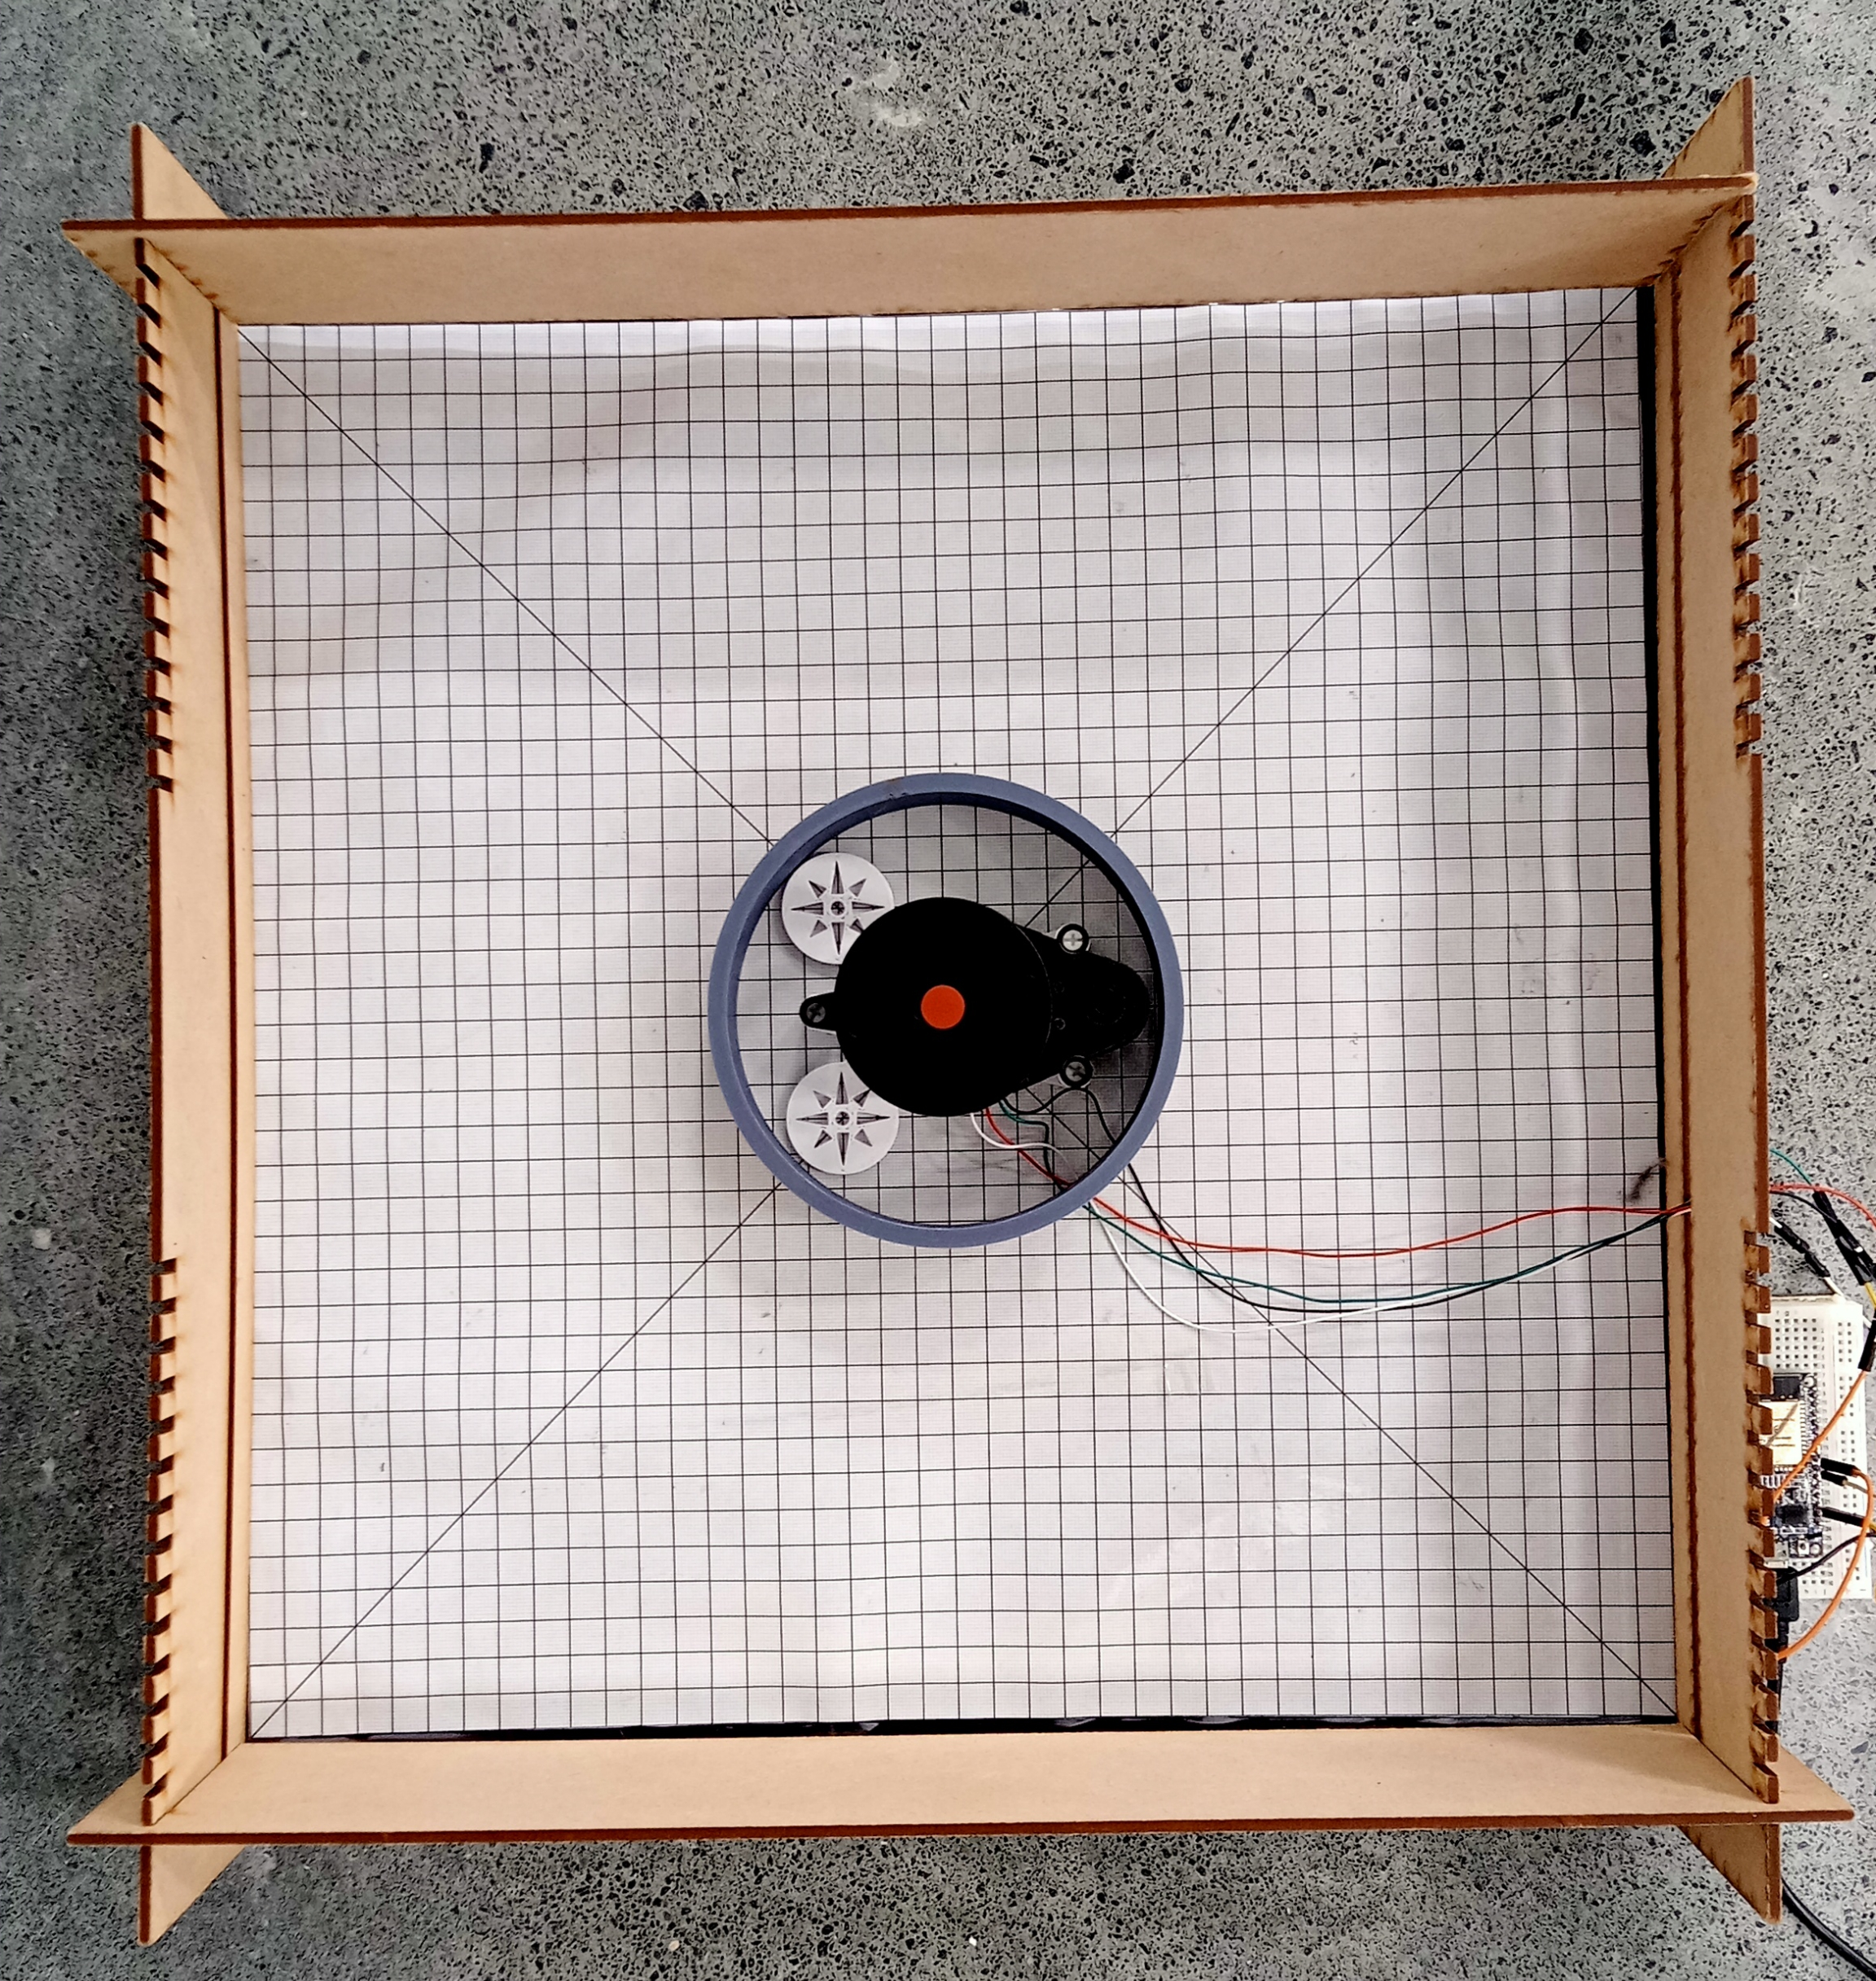
\includegraphics[width=0.65\linewidth]{disposicion_lidar4.jpeg}
		\caption{Disposición del sensor FHL-LD20 dentro del entorno circular: 60 mm de radio.}
		\label{disposicion_lidar4}
		\vspace{1em}
	\end{subfigure}
	\begin{subfigure}{0.45\textwidth}
		\centering
		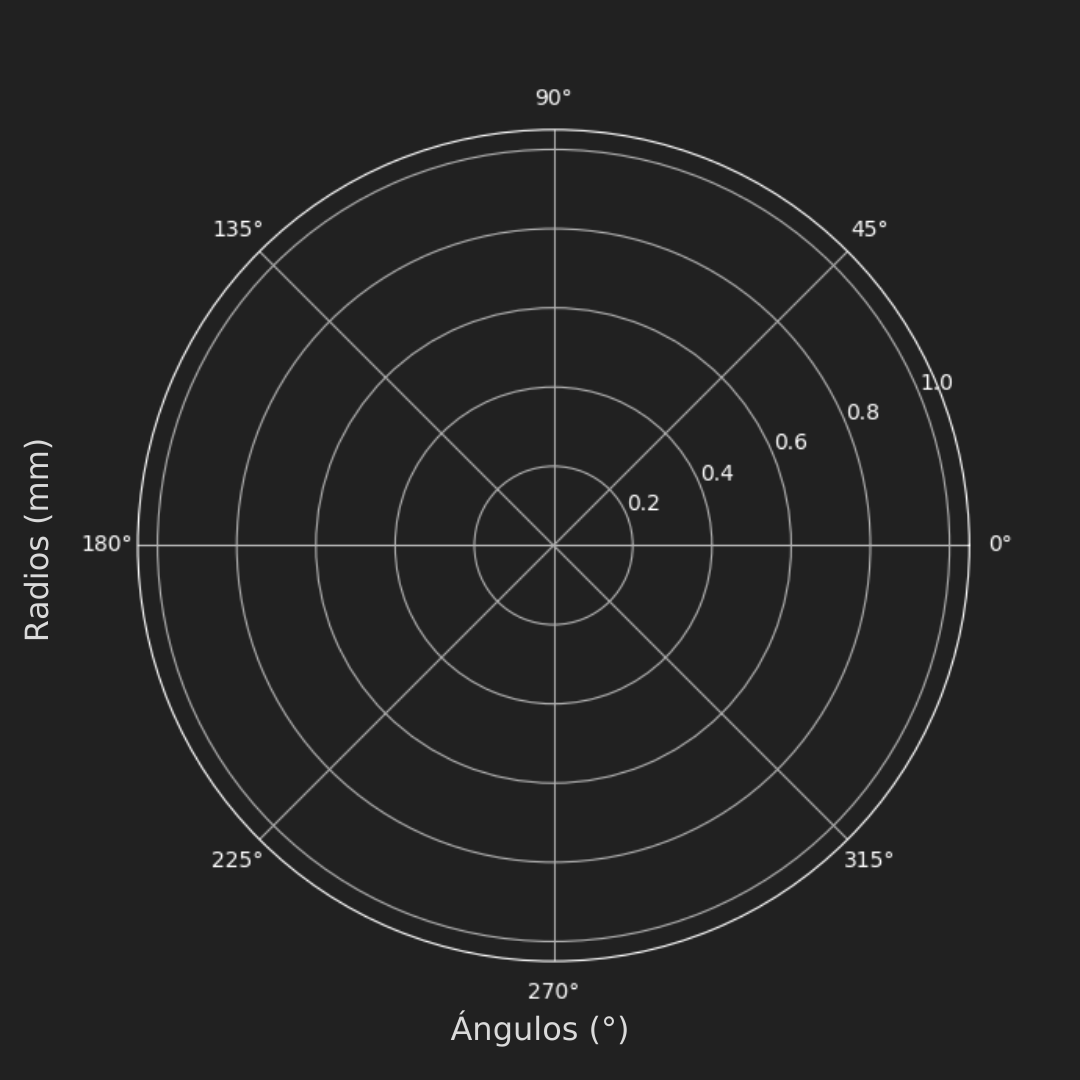
\includegraphics[width=0.9\linewidth]{try_6cm_r.png}
		\caption{Reconstrucción en coordenadas polares de tres revoluciones completas capturadas en entorno circular: 60 mm de radio.}
		\label{try_6cm_r}
	\end{subfigure}
	\hspace{1em}
	\begin{subfigure}{0.45\textwidth}
		\centering
		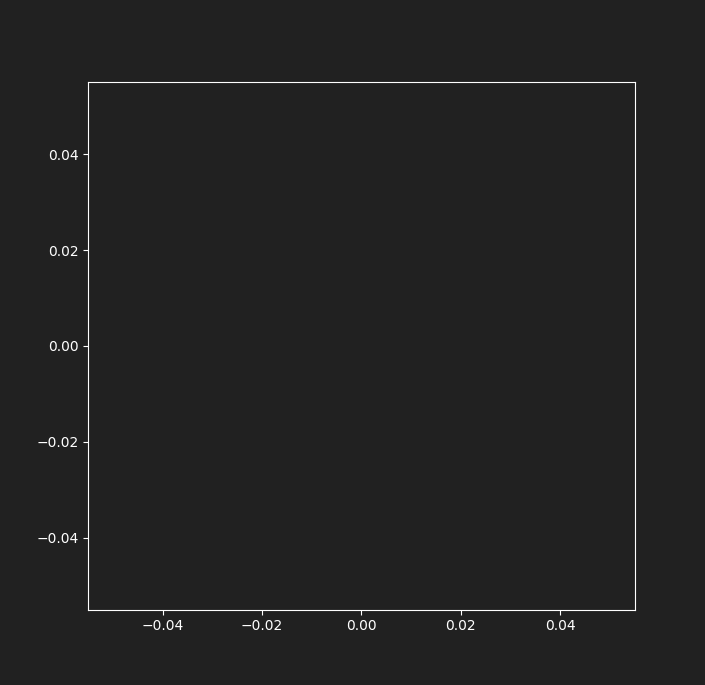
\includegraphics[width=0.9\linewidth]{try_6cm_r_car.png}
		\caption{Reconstrucción en coordenadas cartesianas de tres revoluciones completas capturadas en entorno circular: 60 mm de radio.}
		\label{try_6cm_r_car}
	\end{subfigure}
	\caption{Reconstrucciones vacías de tres revoluciones completas capturadas en entorno circular: 60 mm de radio.}
	\label{fig: reconstrucciones_vacías_6}
\end{figure}

Se llevaron a cabo pruebas adicionales utilizando los contornos circulares de 70, 80, 90 y 100 mm de radio (ver Figuras \ref{fig: reconstrucciones_vacías_7} y \ref{fig: reconstrucciones_vacías_8} en Anexos \ref{min_pruebas}). El entorno circular de 90 mm de radio fue el primero en mostrar indicios de distancias válidas en la reconstrucción. Aunque se logró visualizar una geometría circular, esta presentó irregularidades. Como se observa en la Figura \ref{fig: reconstrucciones_vacías_9}, existen variaciones en la distribución de los puntos capturados.
 
\begin{figure}[H]
	\centering
	\begin{subfigure}{0.6\textwidth}
		\centering
		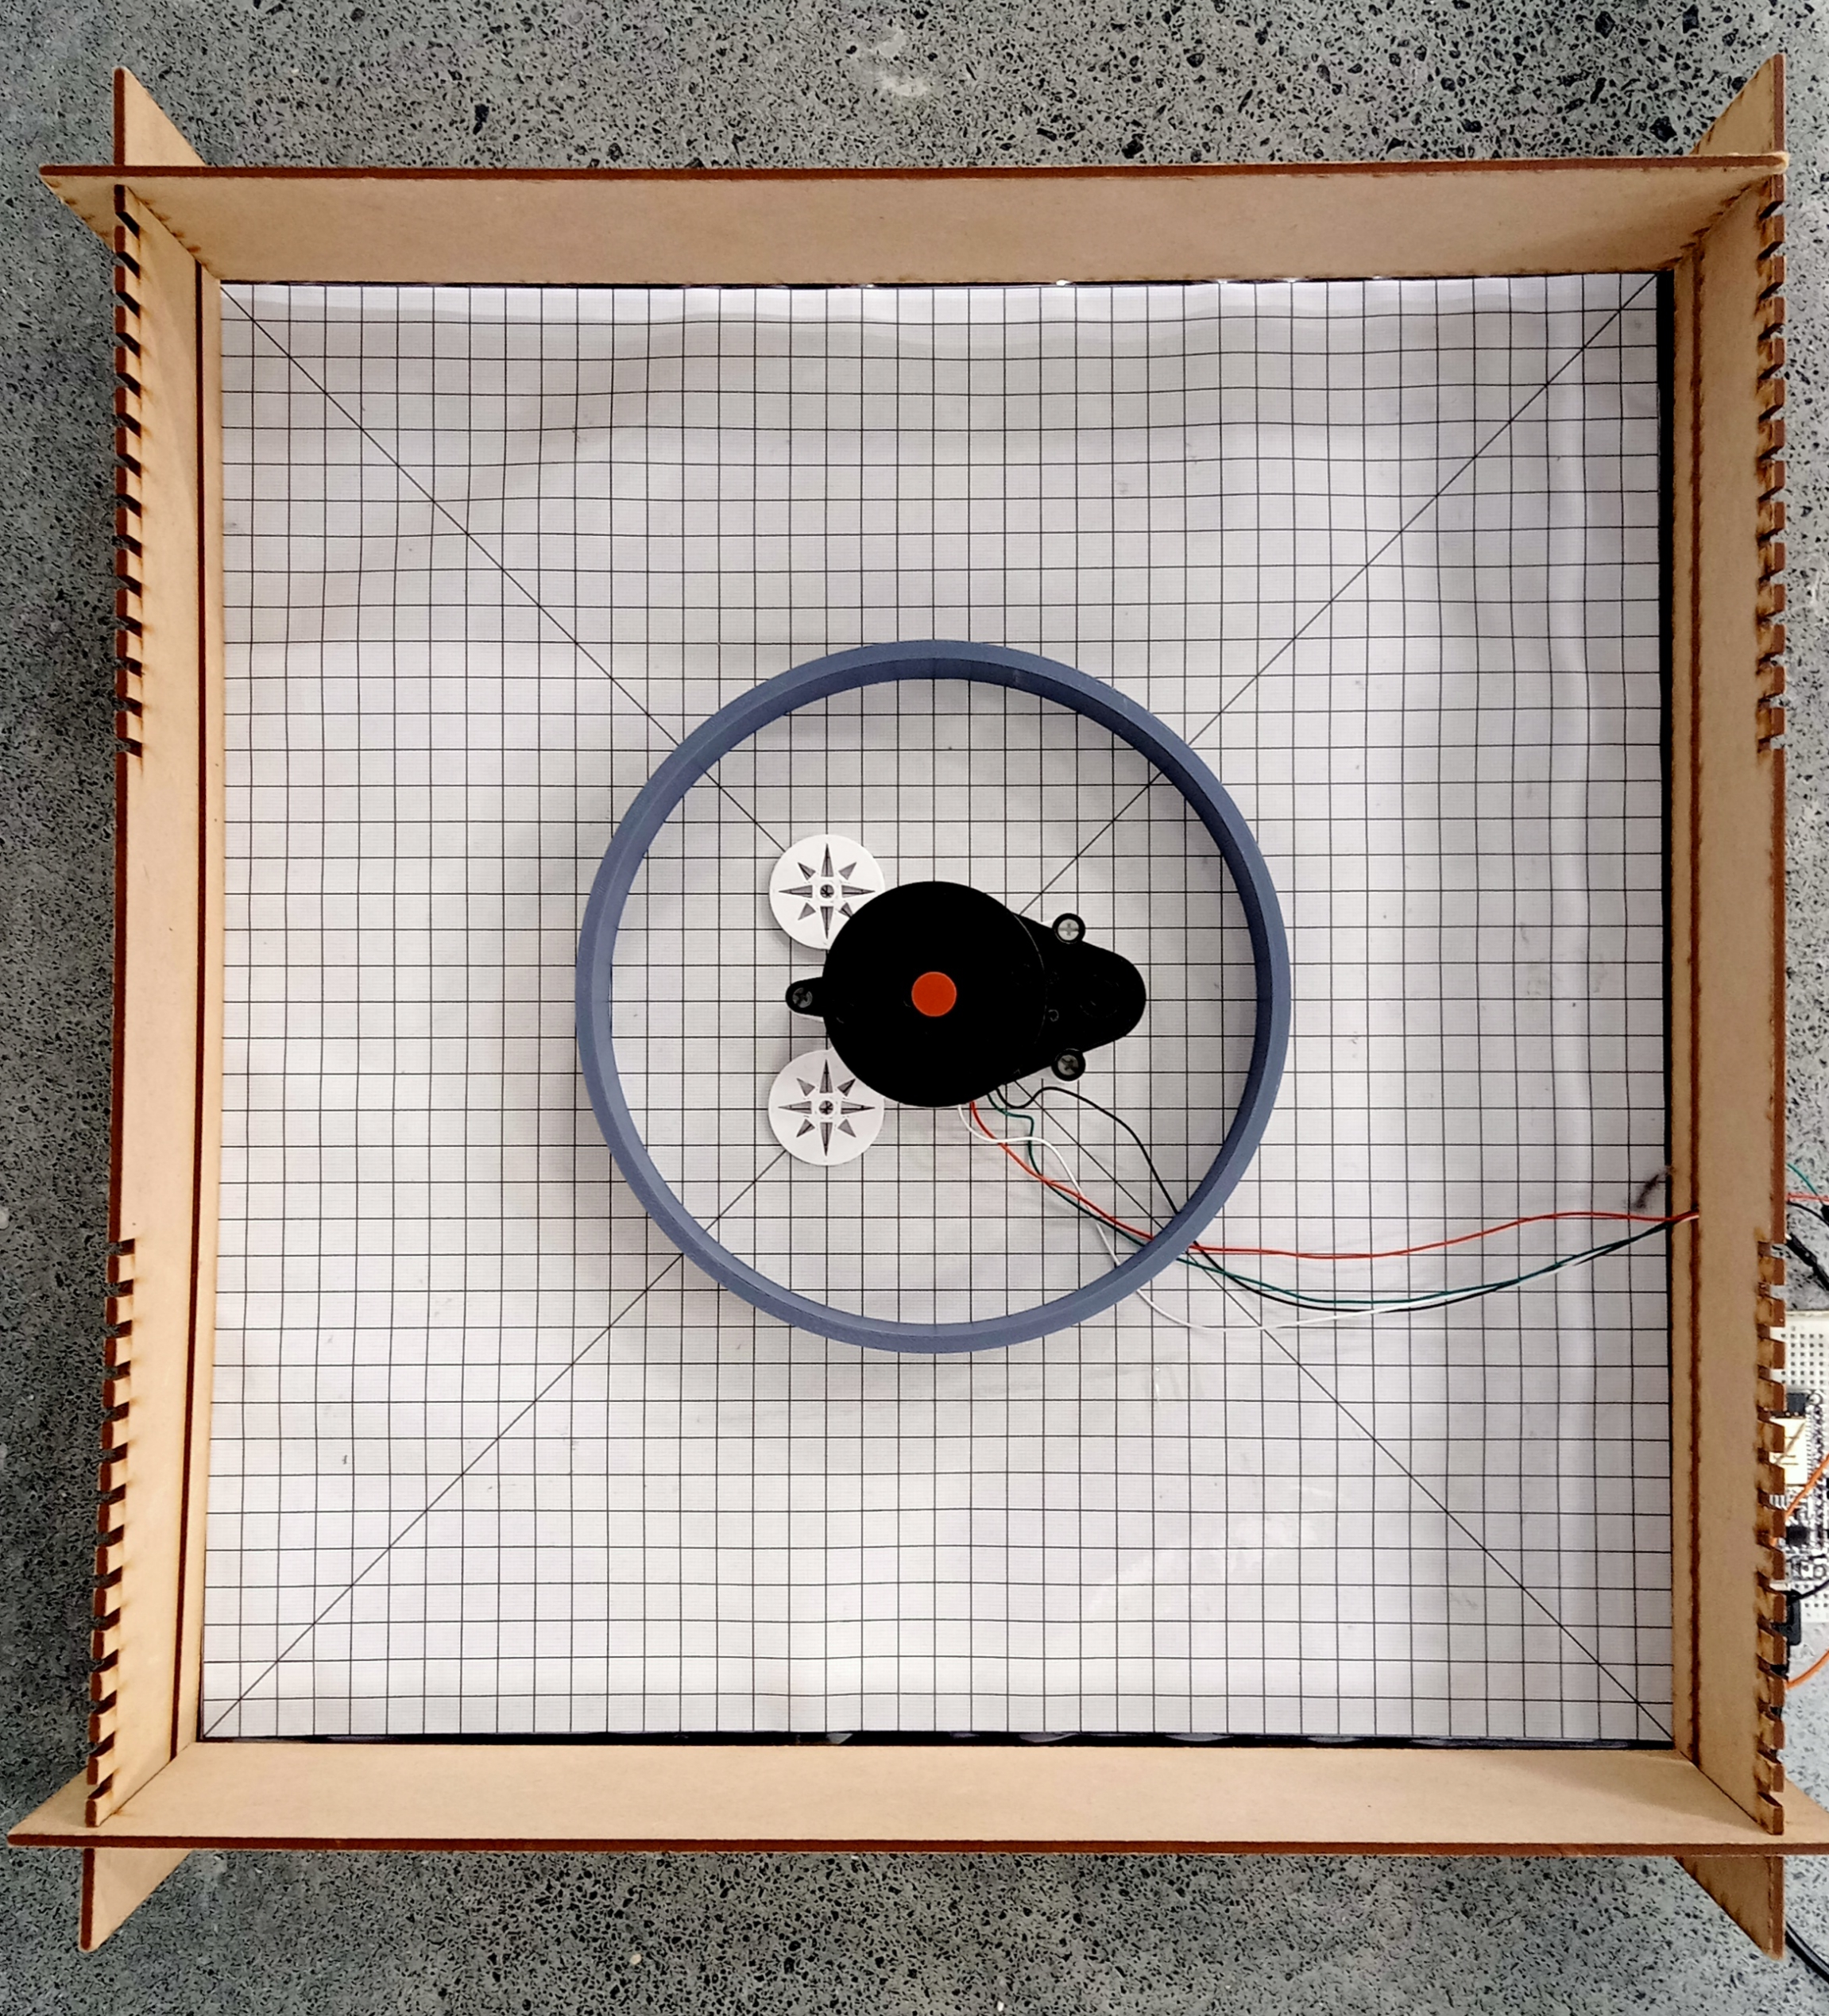
\includegraphics[width=0.6\linewidth]{disposicion_lidar7.jpeg}
		\caption{Disposición del sensor FHL-LD20 dentro del entorno circular: 90 mm de radio}
		\vspace{1em}
	\end{subfigure}
	\begin{subfigure}{0.45\textwidth}
		\centering
		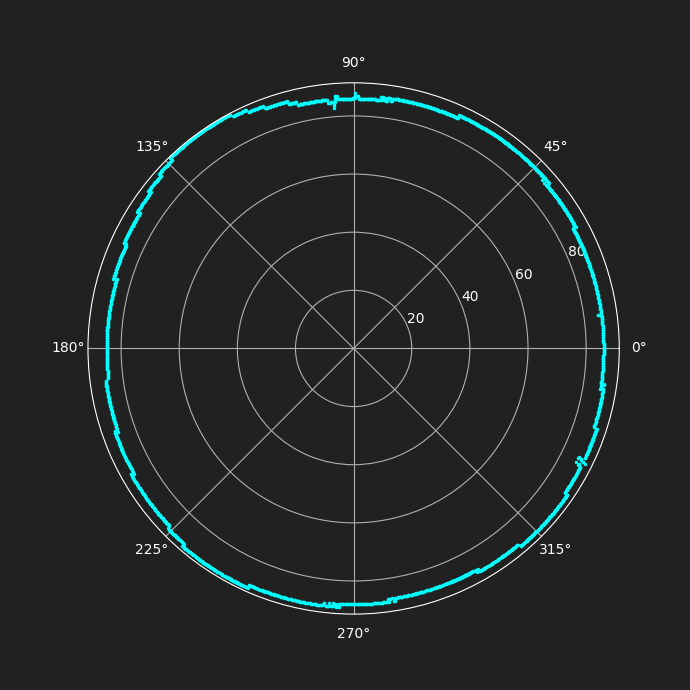
\includegraphics[width=0.8\linewidth]{try_9cm_r.png}
		\caption{Reconstrucción en coordenadas polares de tres revoluciones completas de lectura en entorno circular: 90 mm de radio}
		\label{try_9cm_r}
	\end{subfigure}
	\hspace{1em}
	\begin{subfigure}{0.45\textwidth}
		\centering
		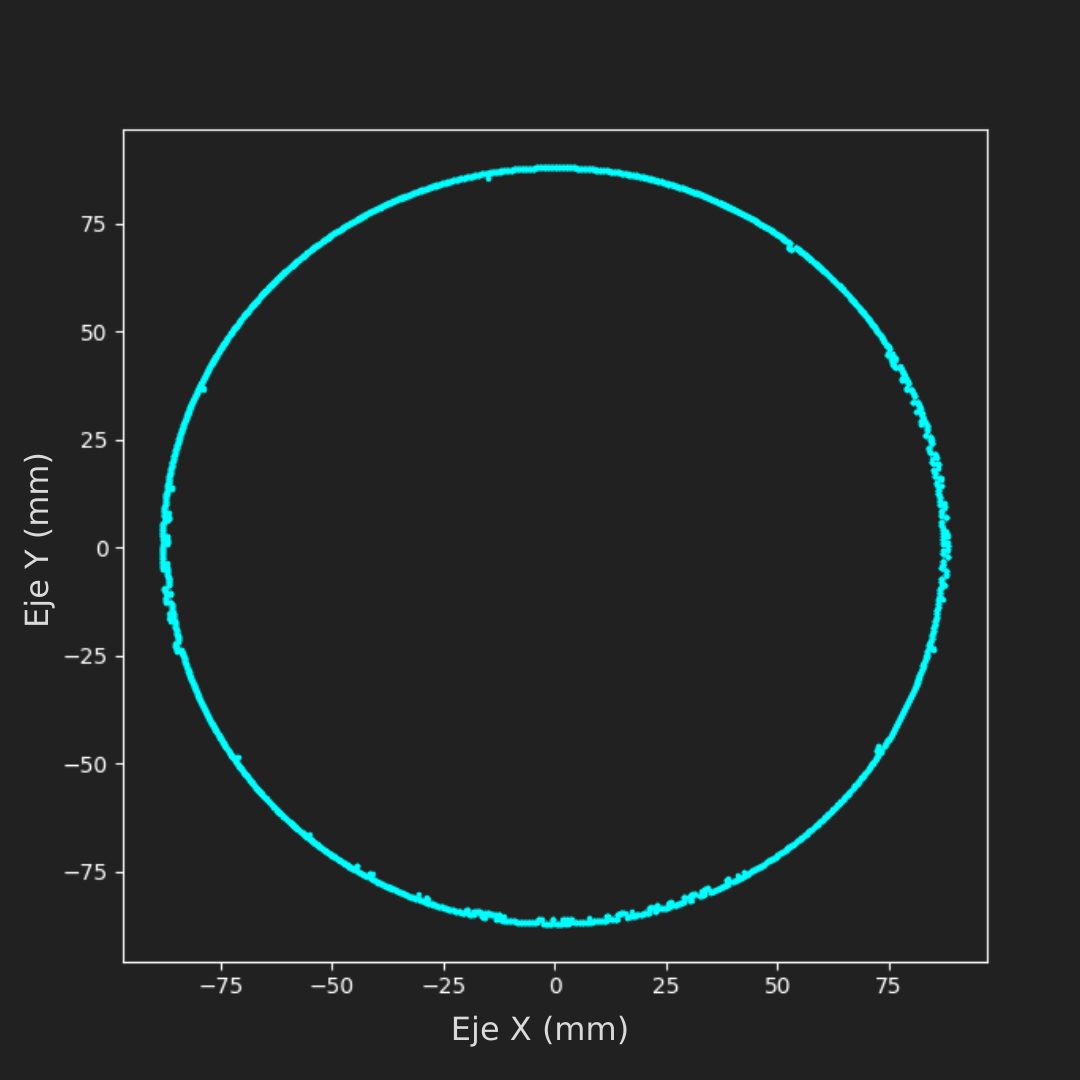
\includegraphics[width=0.8\linewidth]{try_9cm_r_car.png}
		\caption{Reconstrucción en coordenadas cartesianas de tres revoluciones completas de lectura en entorno circular: 90 mm de radio}
		\label{try_9cm_r_car}
	\end{subfigure}
	\caption{Reconstrucción del entorno circular de 90 mm de radio con tres revoluciones completas capturadas.}
	\label{fig: reconstrucciones_vacías_9}
\end{figure}

 
Al realizar la reconstrucción del entorno de 100 mm de radio, se evidenció una geometría más continua y mejor ajustada a la figura esperada. Sin embargo, todavía se observaron ciertas variaciones en la continuidad de la geometría. Al analizar el acabado superficial de los escenarios circulares impresos, se identificó que la rugosidad inherente en las piezas fabricadas pudo influir en la dispersión de las mediciones. Por esta razón, se decidió emplear un material diferente en las pruebas subsecuentes, con el objetivo de minimizar este efecto y mejorar la calidad de las mediciones capturadas. Cabe destacar que, aunque las especificaciones del fabricante indicaban un rango mínimo de medición de 100 mm, el entorno de 90 mm de radio, pese a estar por debajo de este umbral, fue capturado con notable precisión.

\begin{figure}[H]
	\centering
	\begin{subfigure}{0.6\textwidth}
		\centering
		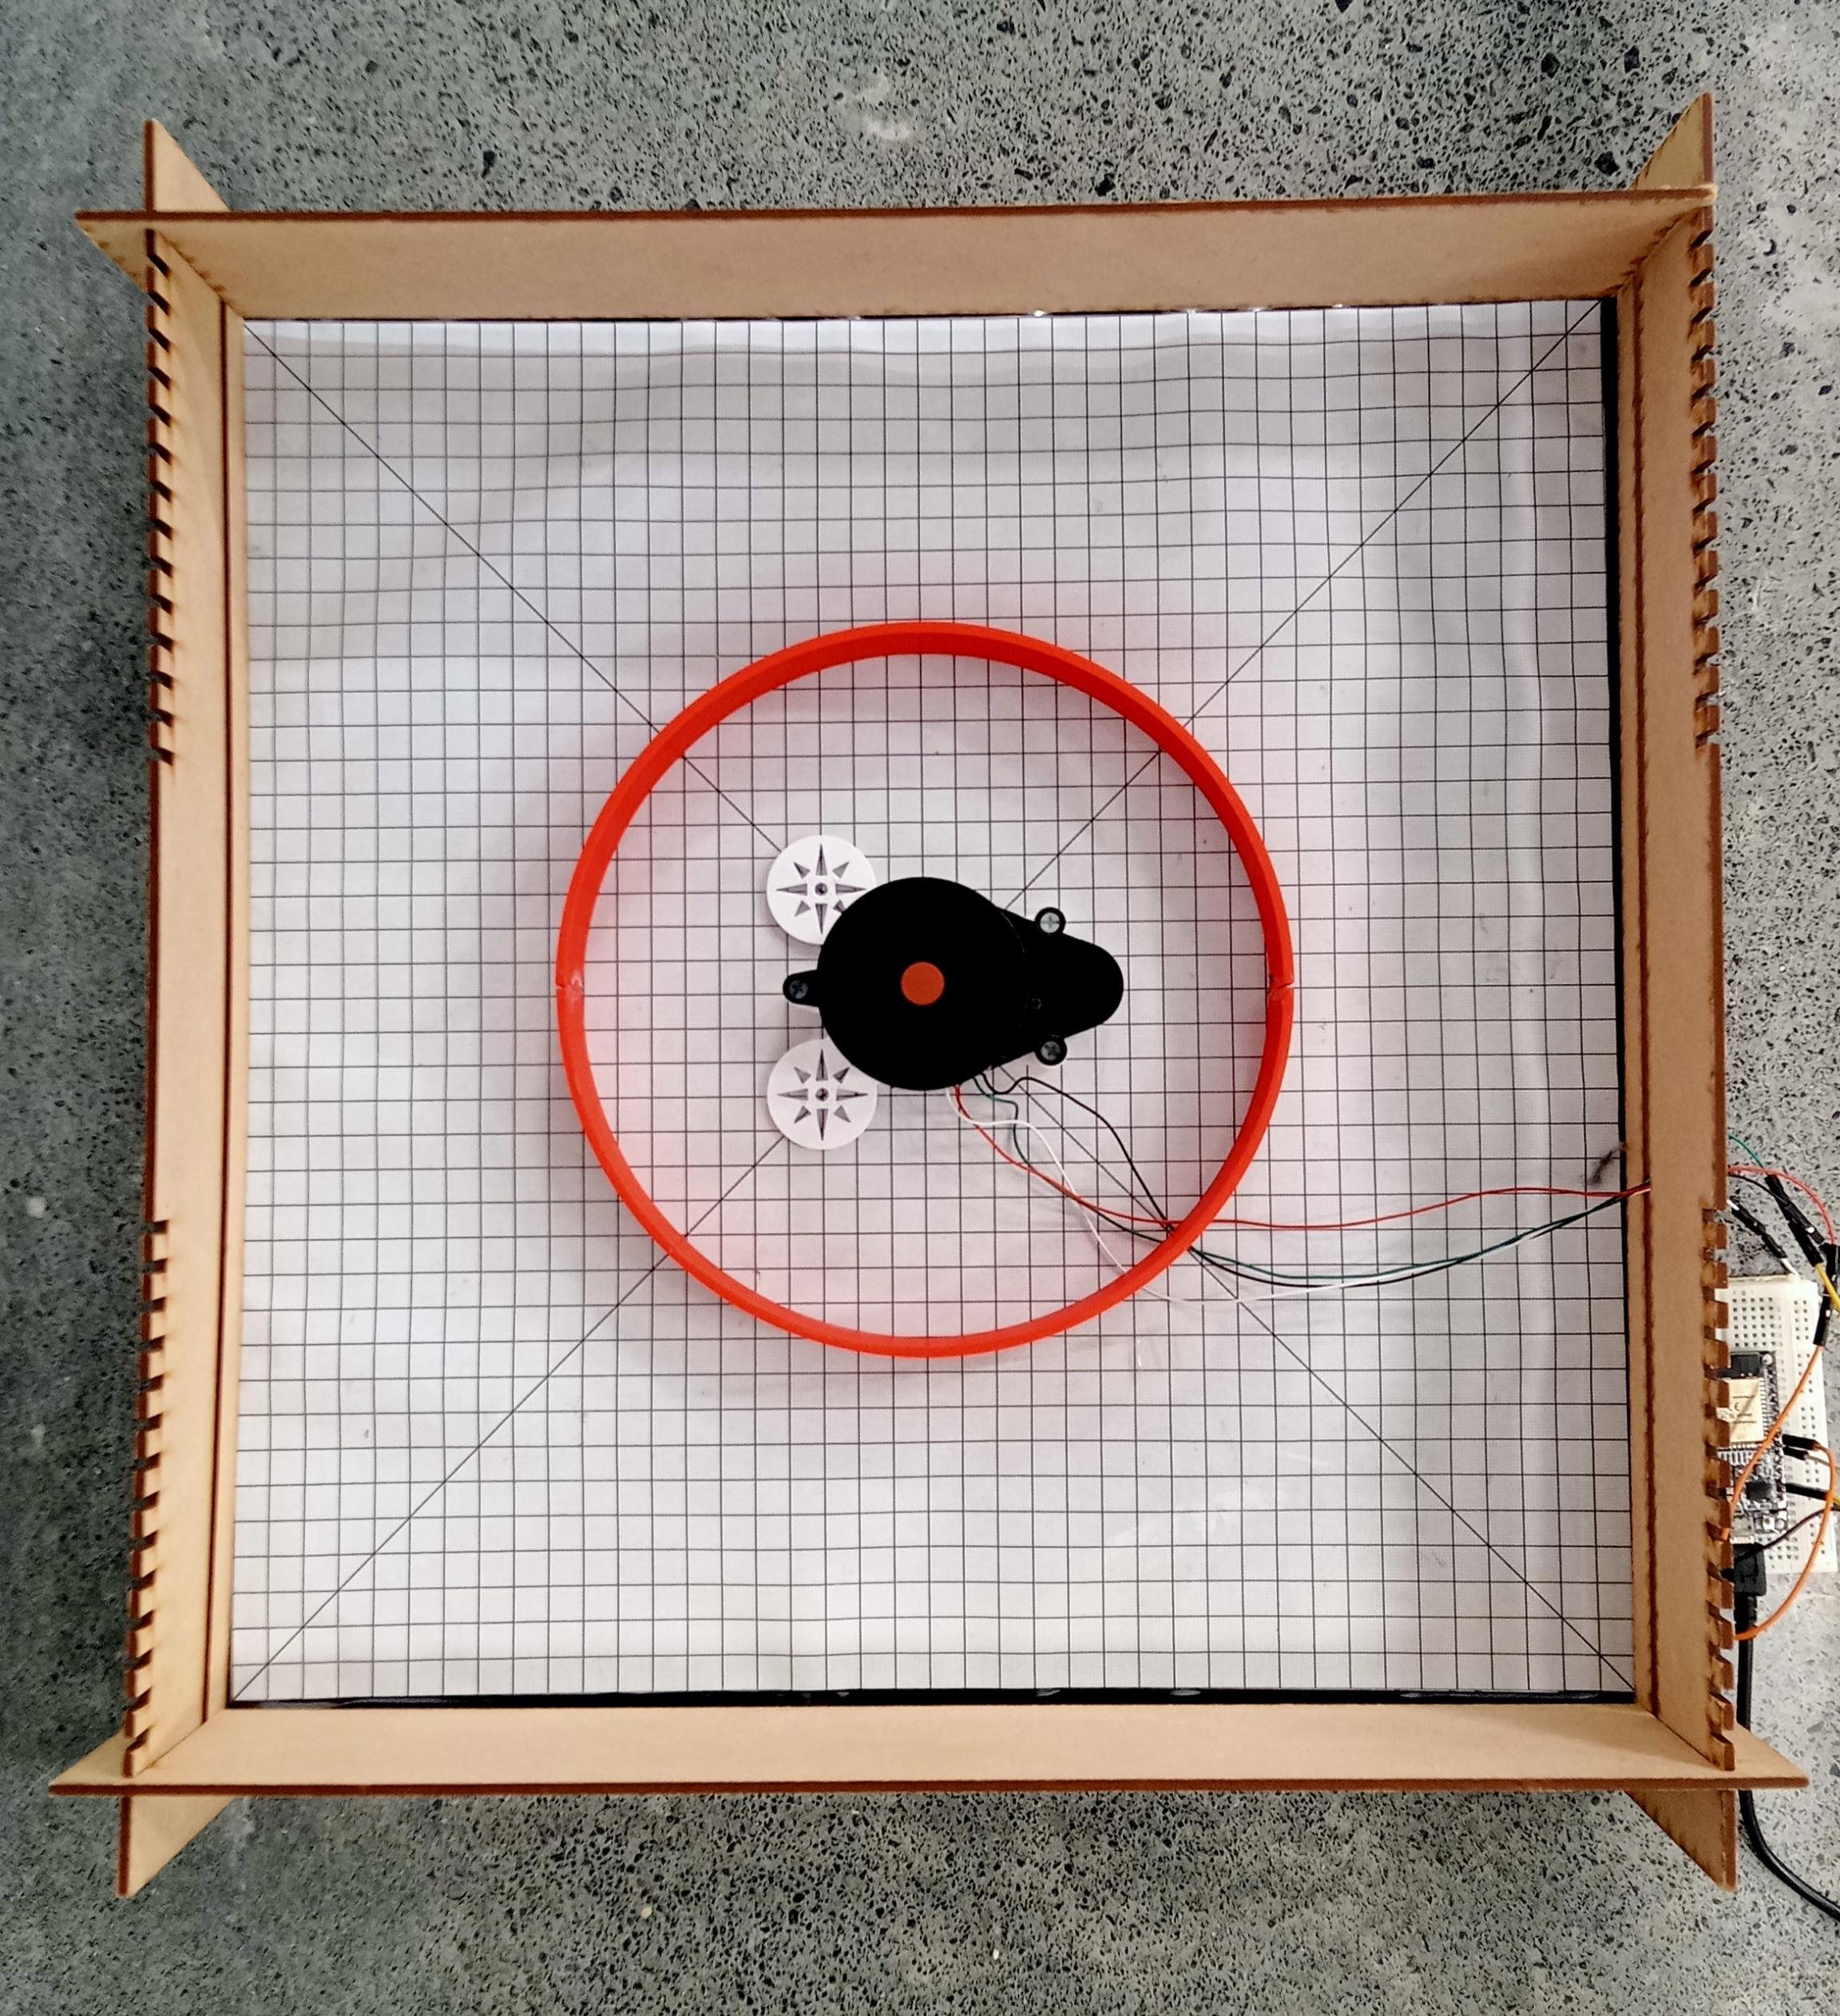
\includegraphics[width=0.65\linewidth]{disposicion_lidar8.jpeg}
		\caption{Disposición del sensor FHL-LD20 dentro del entorno circular: 100 mm de radio.}
		\label{disposicion_lidar8}
		\vspace{1em}
	\end{subfigure}
	\begin{subfigure}{0.45\textwidth}
		\centering
		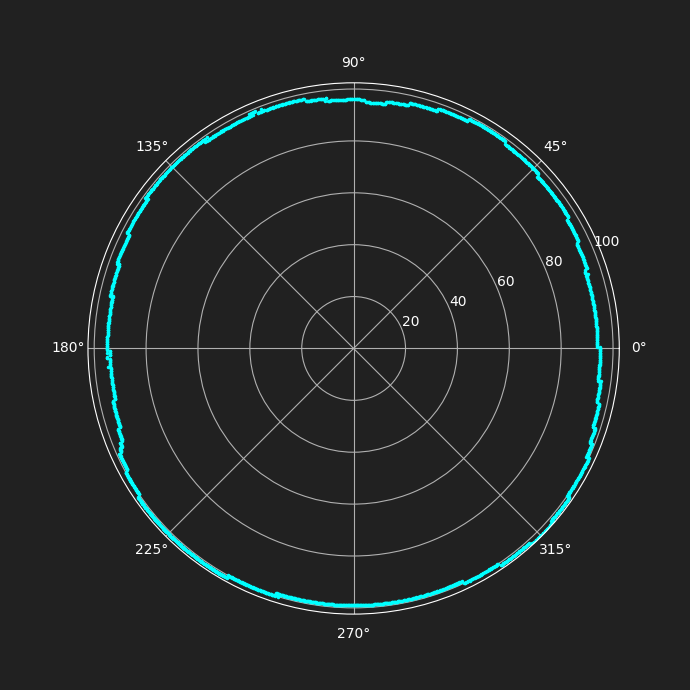
\includegraphics[width=0.9\linewidth]{try_10cm_r.png}
		\caption{Reconstrucción en coordenadas polares de tres revoluciones completas capturadas en entorno circular: 100 mm de radio.}
		\label{try_10cm_r}
	\end{subfigure}
	\hspace{1em}
	\begin{subfigure}{0.45\textwidth}
		\centering
		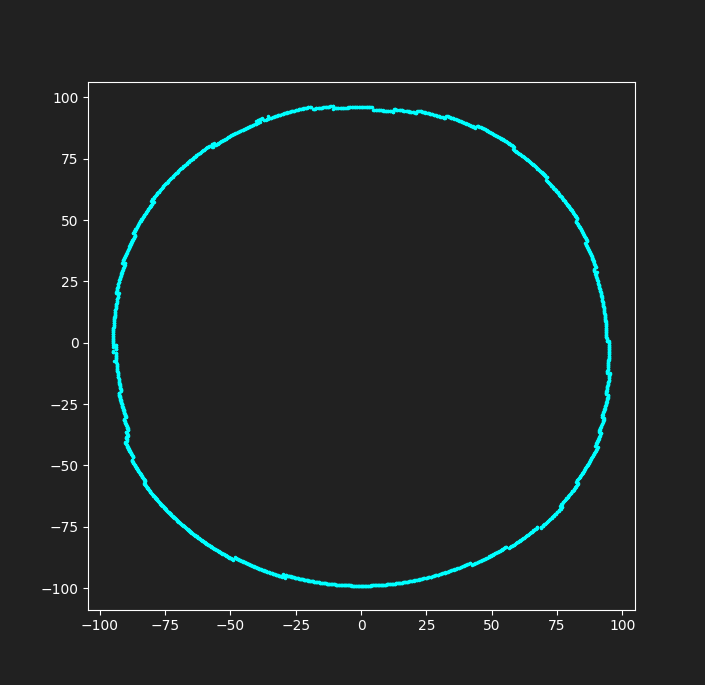
\includegraphics[width=0.9\linewidth]{try_10cm_r_car.png}
		\caption{Reconstrucción en coordenadas cartesianas de tres revoluciones completas capturadas en entorno circular: 100 mm de radio.}
		\label{try_10cm_r_car}
	\end{subfigure}
	\caption{Reconstrucción del entorno circular de 100 mm de radio con tres revoluciones completas capturadas.}
	\label{fig: reconstrucciones_10}
\end{figure}

Para garantizar una detección eficiente y reducir el ruido causado por los componentes estructurales de los agentes robóticos donde se integrará el sensor, como es el caso del Pololu 3pi+, se ha establecido un rango mínimo de medición de 15 cm. A distancias inferiores a esta, el sensor podría captar partes del propio robot, lo que afectaría negativamente la precisión de las mediciones. Además, dado que la probabilidad de encontrar obstáculos relevantes a menos de 10 cm en el entorno de operación es baja, establecer este límite permite enfocarse en la detección de obstáculos que realmente impacten en la navegación del agente robótico.

\section{Estimación de las varianzas del sensor }
\label{sec:estimacion}
En aplicaciones de mapeo de entornos con agentes robóticos móviles, la localización del robot depende de mediciones de distancia y ángulo hacia puntos de referencia fijos (\textit{landmarks}). Describir cómo un sensor de distancia, como un LIDAR, mide su posición relativa con respecto a estos puntos resulta esencial para construir un mapa coherente y actualizar la posición del robot en función de sus observaciones. Este enfoque permite corregir errores acumulados de odometría y reducir la incertidumbre en la estimación de posición, lo que posibilita que los agentes robóticos se localicen y mapeen su entorno de manera precisa y confiable \cite{corke_robotics_2017}. Para modelar matemáticamente las observaciones de un sensor de distancia equipado en un agente robótico, se emplea la Ecuación \eqref{eq:robot_landmark}.

\begin{equation}
	\label{eq:robot_landmark}
	z = h(x,p_i) 
\end{equation}

donde $x = (x_v, y_v, \theta_v)^T$ representa el estado del agente robótico, con $x_v$ y $y_v$ como sus coordenadas en el sistema global y $\theta_v$ como su orientación. Mientras que $p_i = (x_i, y_i)^T$ denota la posición conocida del i-ésimo punto de referencia en el entorno. Para modelar la incertidumbre en las mediciones de distancia y ángulo, la Ecuación \eqref{eq:robot_landmark2} extiende el modelo de observación, añadiendo un vector de ruido que refleja los errores en estas mediciones.

\begin{equation}
	\label{eq:robot_landmark2}
	z = h(x, p_i) =
	\begin{pmatrix}
		\sqrt{(y_i - y_v)^2 + (x_i - x_v)^2} \\
		\tan^{-1}\left(\frac{y_i - y_v}{x_i - x_v}\right) - \theta_v
	\end{pmatrix}
	+
	\begin{pmatrix}
		w_r \\
		w_\beta
	\end{pmatrix}
\end{equation}

\begin{equation}
	\label{eq:matriz_covarianza}
	\begin{pmatrix}
		w_r \\
		w_\beta
	\end{pmatrix}
	\sim
	N(0,W),	W =
	\begin{pmatrix}
		\sigma_r^2 & 0 \\
		0 & \sigma_\beta^2
	\end{pmatrix}
\end{equation}

Esta ecuación describe cómo el sensor mide la distancia $r$ y el ángulo $\beta$ al punto de referencia $p_i$, incorporando un vector de ruido en las mediciones. Este modelo asume que los errores $w_r$ y $w_\beta$ siguen  una distribución Gaussiana con media cero y varianza conocida en las mediciones de distancia y ángulo, respectivamente. En la Ecuación \ref{eq:matriz_covarianza} se especifica la matriz de covarianza $W$, en la cual $\sigma_r^2$ representa la varianza del error en la distancia y $\sigma_\beta^2$ la varianza del error en el ángulo. Esta matriz de covarianza refleja que las observaciones del sensor están sujetas a una incertidumbre inherente.

Para estimar las varianzas $\sigma_r^2$ y $\sigma_\beta^2$ se llevaron a cabo dos experimentos con el sensor LIDAR FHL-LD20.  El primero se centró en evaluar la varianza asociada a las mediciones de distancia, mientras que el segundo se enfocó en analizar las mediciones angulares. Ambos experimentos fueron diseñados para proporcionar una comprensión más profunda del rendimiento del sensor y su precisión en condiciones de operación.

\subsection{Estimación de la varianza asociada a las mediciones de distancia del sensor}
\label{var_dist}
Para el primer experimento, se diseñaron ocho círculos concéntricos con radios de 150, 200, 250, 300, 350, 400, 450 y 500 mm, todos con una altura de 70 mm. Estos círculos fueron fabricados en MDF y recubiertos con una capa uniforme de cartón de 1 mm de grosor. Además, se imprimió una cuadrícula de 1.2$\times$1.2 metros, dividida en intervalos de un centímetro. Esta cuadrícula incluía una serie de círculos concéntricos con los radios mencionados y líneas diagonales que cruzaban su centro, creando un sistema de referencia radial. En conjunto, este diseño ofreció un entorno controlado para analizar las mediciones en coordenadas polares y cartesianas.

\begin{figure}[H]
	\centering
	\begin{subfigure}{\textwidth}
		\centering
		\makebox[\textwidth]{\includegraphics[width=0.6\linewidth]{disposicion_lidar_var_dist1.jpg}}
		\caption{Disposición del sensor FHL-LD20 dentro del entorno circular: 149 mm de radio}
		\label{fig:disposicion_lidar_var1}
		\vspace{1em}
	\end{subfigure}
	\begin{subfigure}{0.45\textwidth}
		\centering
		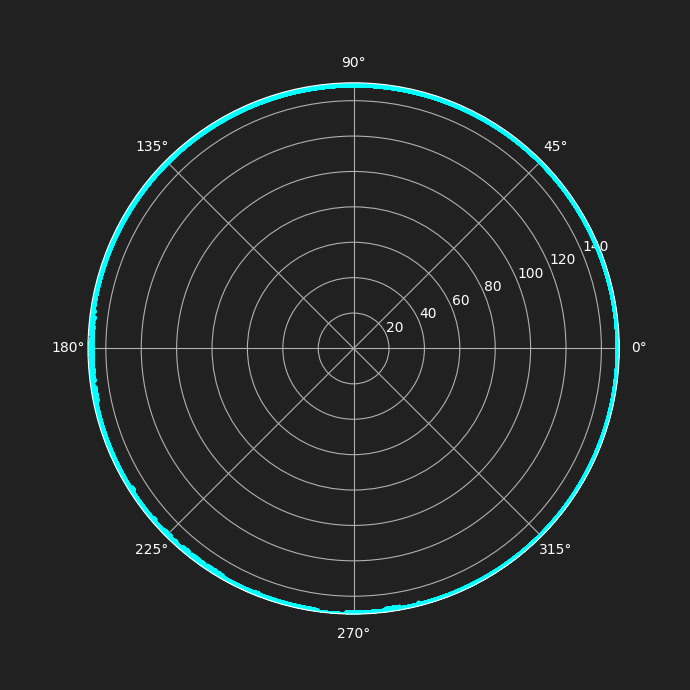
\includegraphics[width=0.8\linewidth]{0.149m_radius.png}
		\caption{Reconstrucción en coordenadas polares de entorno circular: 149 mm de radio}
		\label{fig:149m_radius_xy}
	\end{subfigure}
	\hspace{1em}
	\begin{subfigure}{0.45\textwidth}
		\centering
		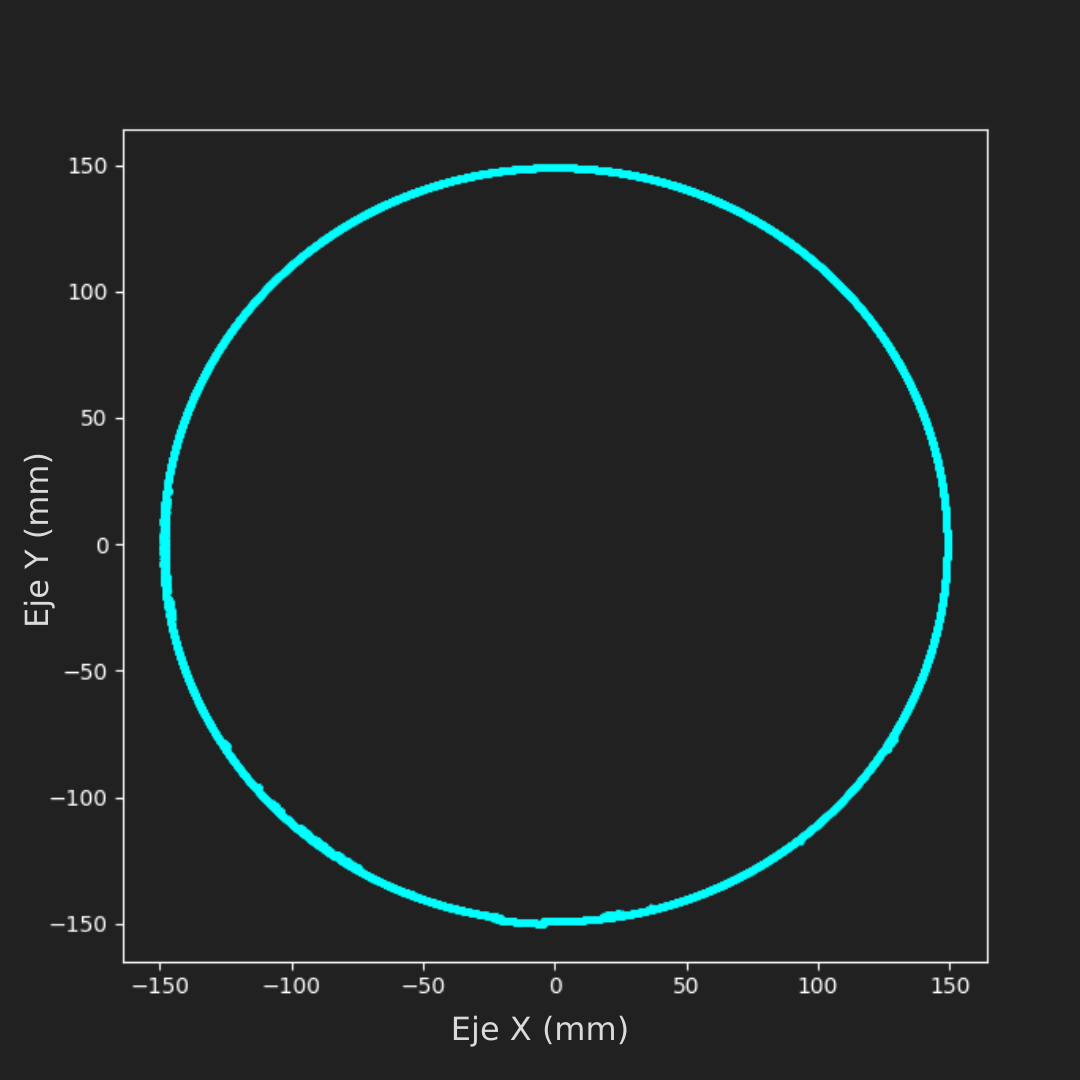
\includegraphics[width=0.83\linewidth]{0.149m_radius_XY.png}
		\caption{Reconstrucción en coordenadas cartesianas de entorno circular: 149 mm de radio}
		\label{fig:149m_radius}
	\end{subfigure}
	\caption{Reconstrucción con 180 revoluciones completas capturadas del entorno circular: 149 mm de radio.}
	\label{fig:disposicion_lidar_var_dist1}
\end{figure}

\begin{figure}[H]
	\centering
	\begin{subfigure}{\textwidth}
		\centering
		\makebox[\textwidth]{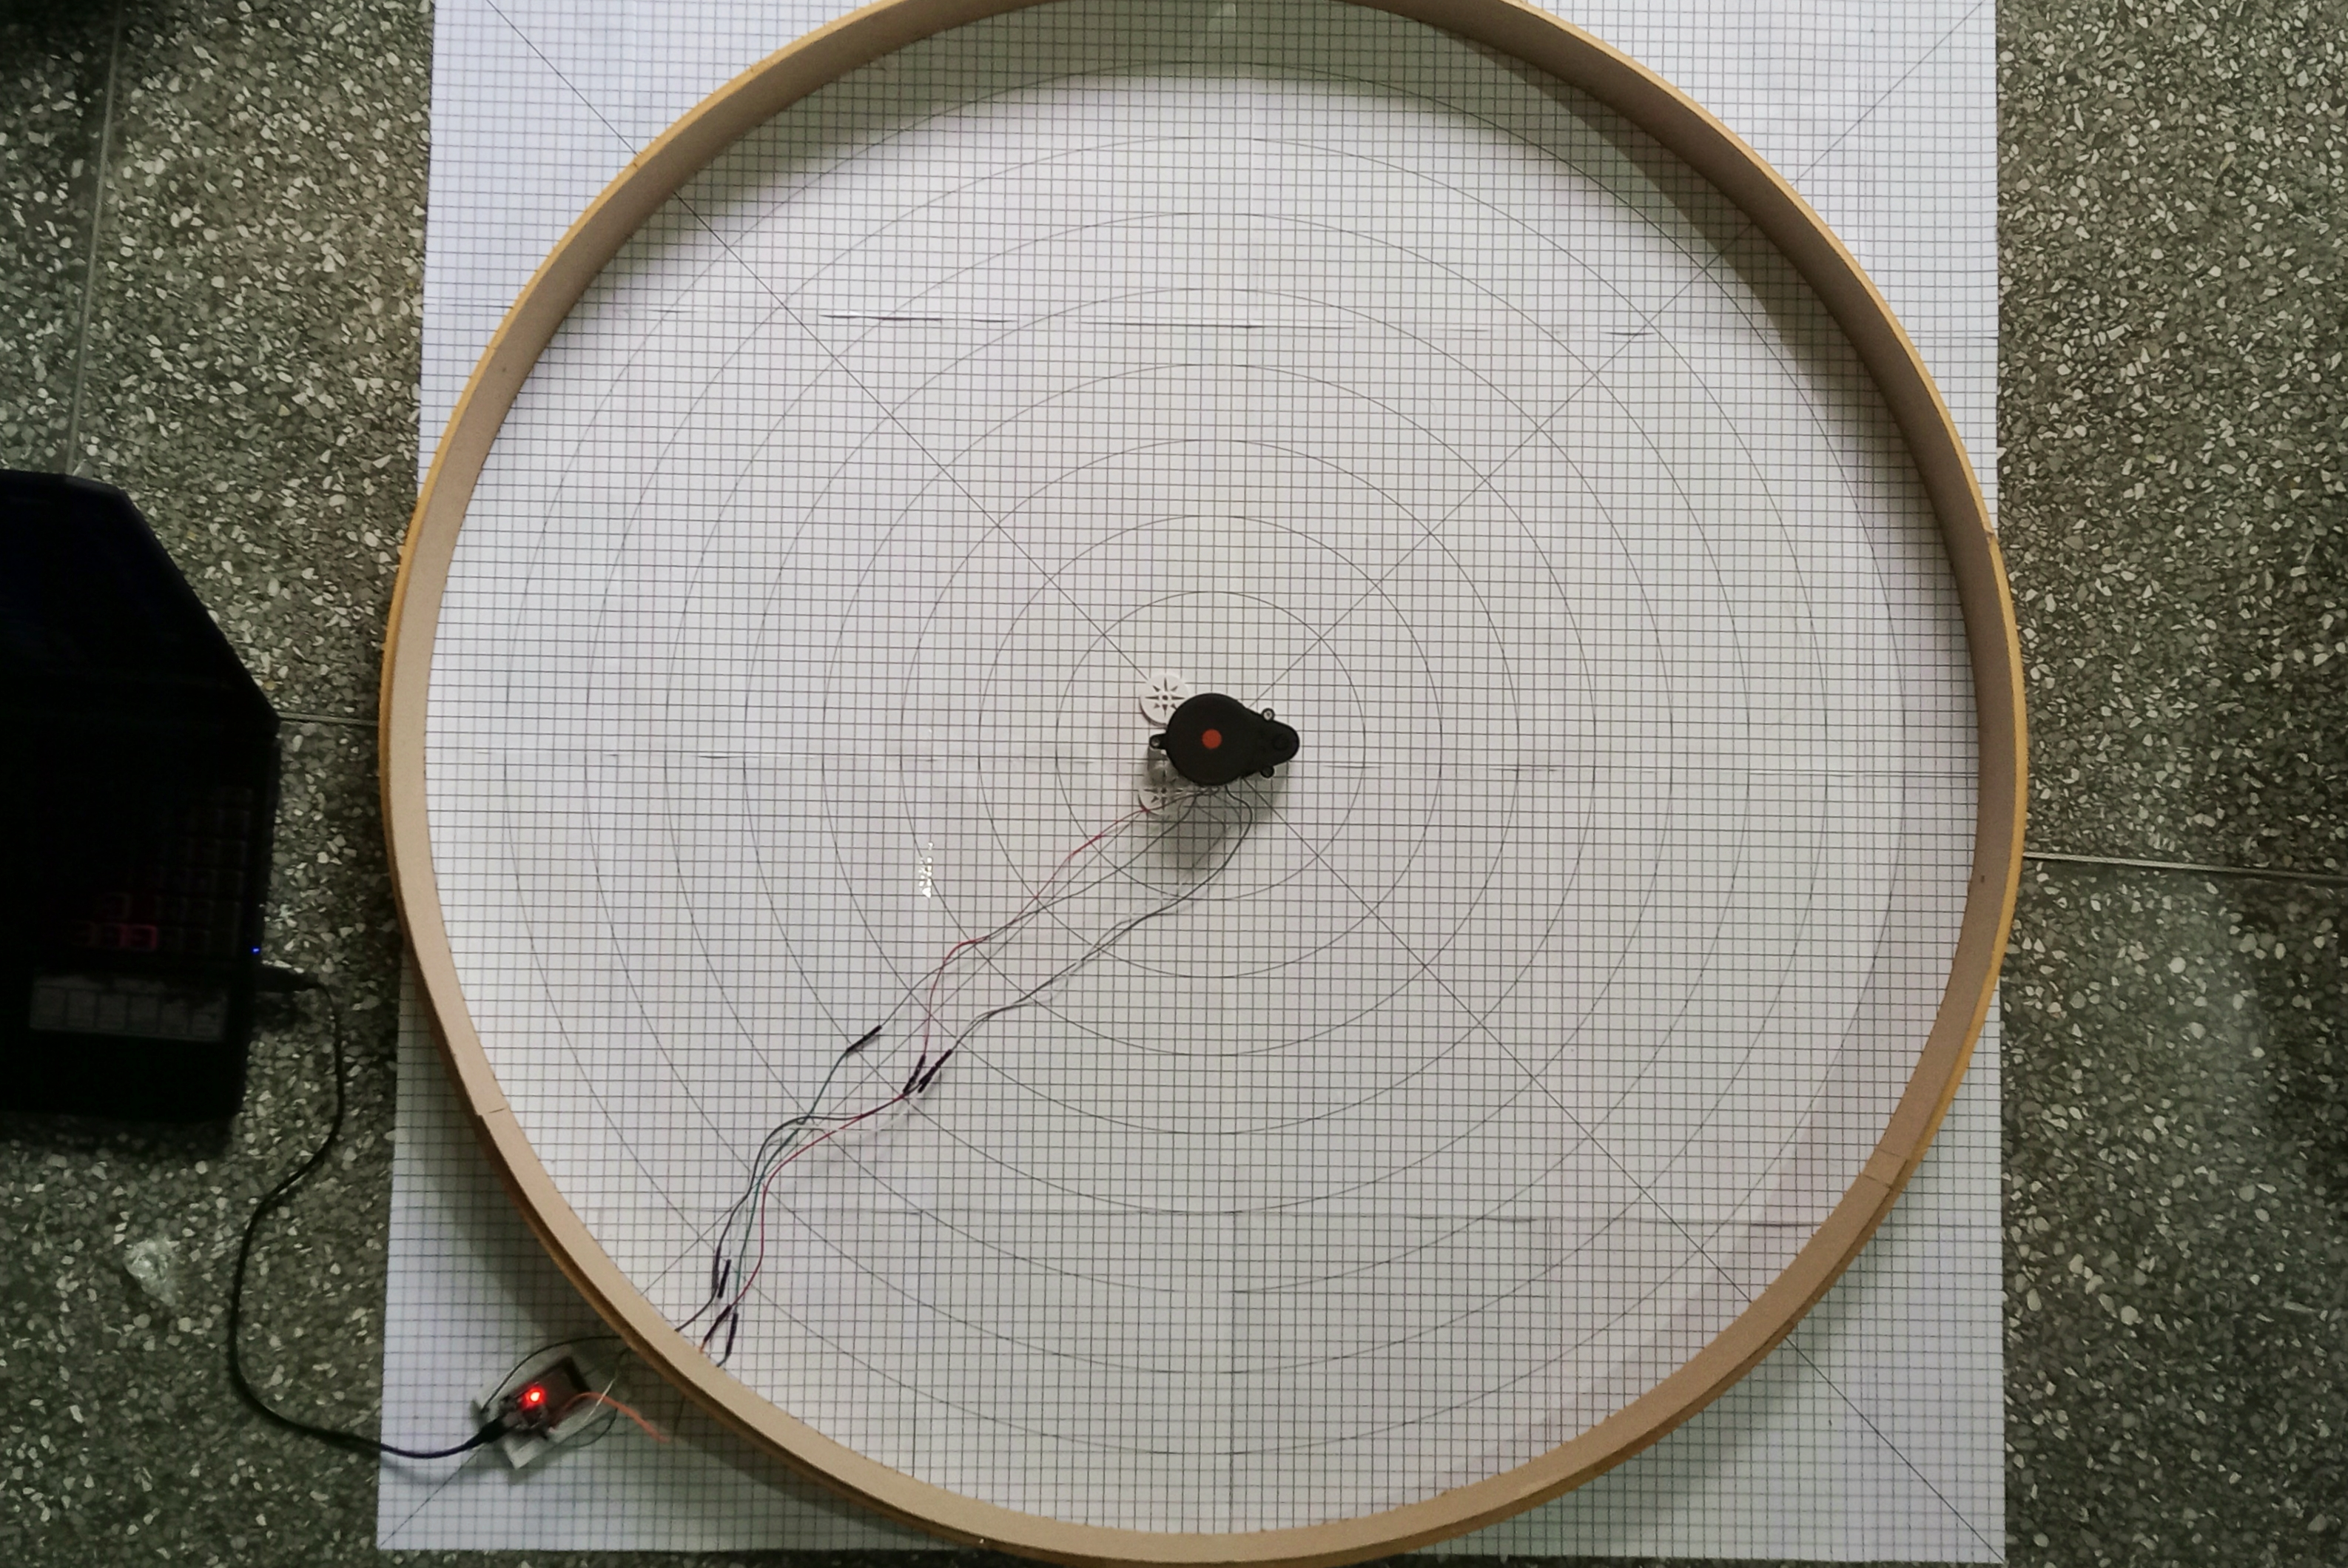
\includegraphics[width=0.6\linewidth]{disposicion_lidar_var_dist8.jpg}}
		\caption{Disposición del sensor FHL-LD20 dentro del entorno circular: 499 mm de radio}
		\label{fig:disposicion_lidar_var8}
		\vspace{1em}
	\end{subfigure}
	\begin{subfigure}{0.45\textwidth}
		\centering
		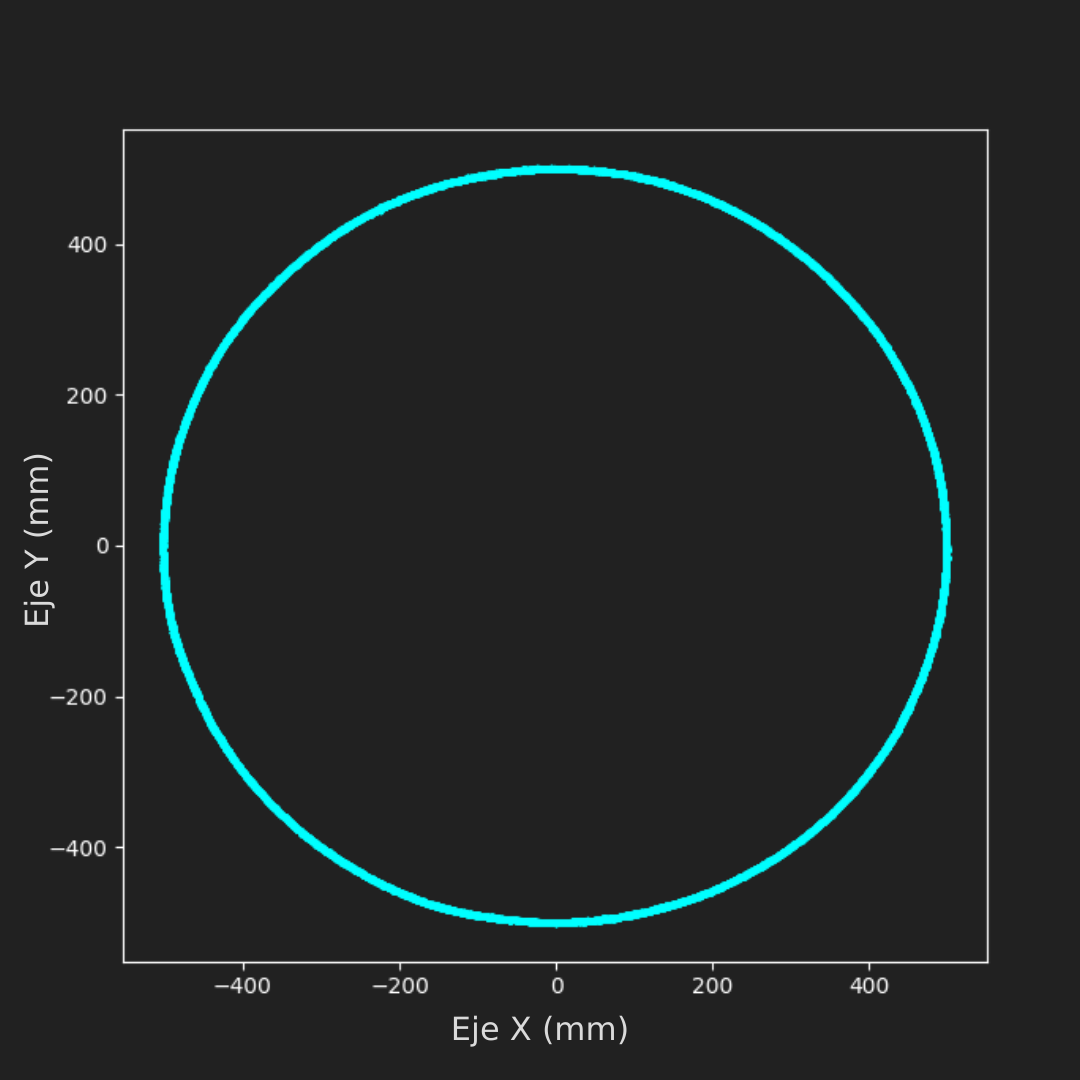
\includegraphics[width=0.8\linewidth]{0.499m_radius.png}
		\caption{Reconstrucción en coordenadas polares de entorno circular: 499 mm de radio}
		\label{fig:499m_radius_xy}
	\end{subfigure}
	\hspace{1em}
	\begin{subfigure}{0.45\textwidth}
		\centering
		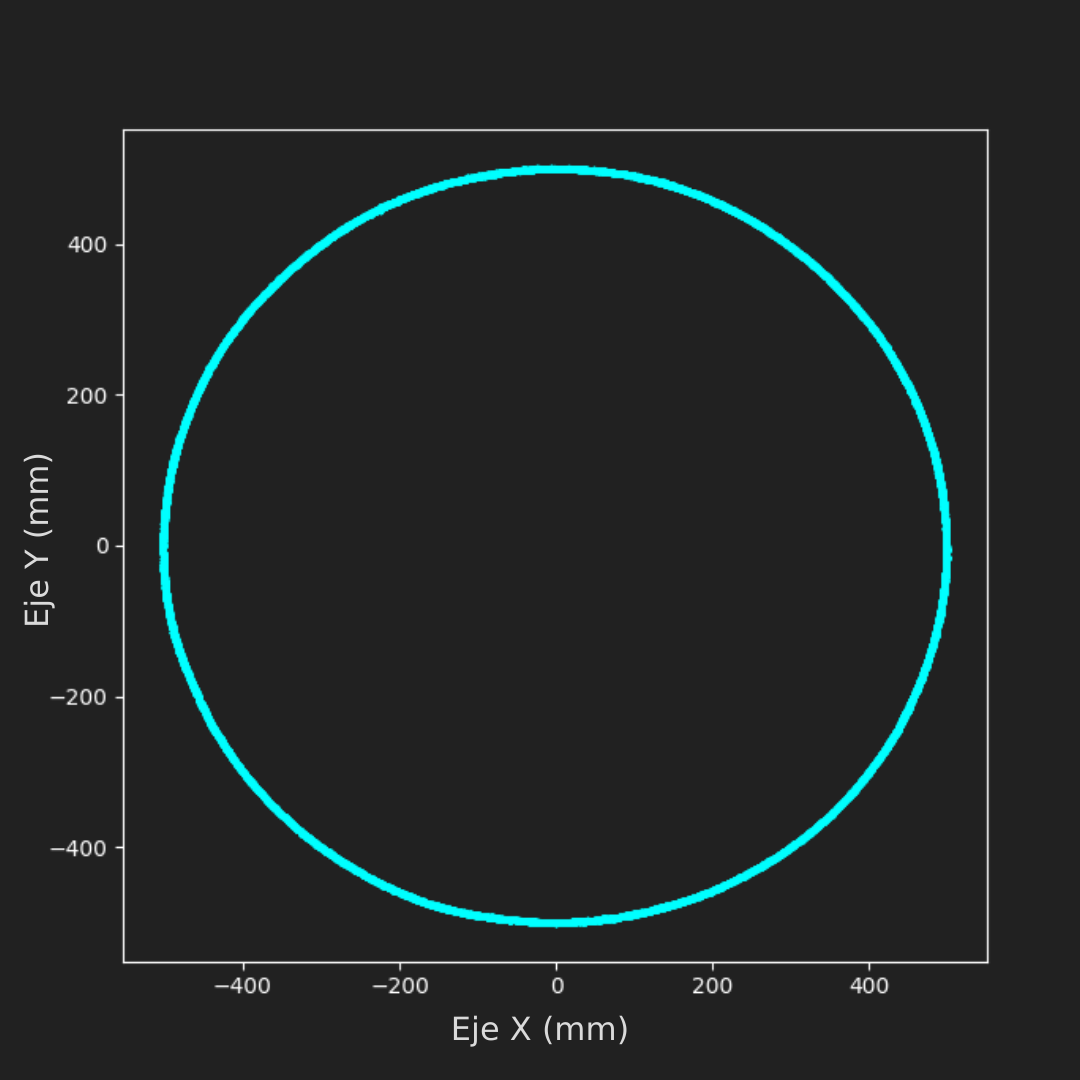
\includegraphics[width=0.83\linewidth]{0.499m_radius_XY.png}
		\caption{Reconstrucción en coordenadas cartesianas de entorno circular: 499 mm de radio}
		\label{fig:499m_radius}
	\end{subfigure}
	\caption{Reconstrucción del entorno circular de 499 mm de radio con 180 revoluciones completas capturadas.}
	\label{fig:disposicion_lidar_var_dist8}
\end{figure}

Como se muestra en las Figuras \ref{fig:disposicion_lidar_var_dist1} y \ref{fig:disposicion_lidar_var_dist8}, el sensor se posicionó en el centro de la cuadrícula y se alineó concéntricamente uno de los círculos fabricados, utilizando las líneas radiales como guía. Con esta disposición se esperaba que el sensor registrara mediciones uniformes a lo largo de todo el perímetro del círculo. Después de capturar un total de 180 revoluciones, equivalente a 129,600 puntos de medición, y repetir diez veces las mediciones, fue posible establecer el promedio, varianza muestral y sesgo asociados con las distancias medidas por el sensor para cada círculo. El análisis de los datos obtenidos con los ocho círculos permitió evaluar la la precisión del sensor a distintas distancias, proporcionando una base sólida para caracterizar la variabilidad en las mediciones y determinar la varianza asociada en cada caso.

Los resultados del experimento se presentan en el Cuadro \ref{cuadro:stats}, donde se muestran las varianzas calculadas para cada uno de los ocho radios evaluados. En todos los casos, se verificó que las mediciones se ajustaran a una distribución gaussiana normal (ver Figuras \ref{fig:histograma_dists1} a \ref{fig:histograma_dists2} en Anexos \ref{varianza_distancia}), lo que respalda la validez del modelo de ruido asumido para las observaciones del sensor (Sección \ref{sec:estimacion}). Además, se observó que, a medida que aumentaba la distancia de los radios, también se incrementaba la varianza en las mediciones, indicando una disminución gradual en la exactitud del sensor. Para caracterizar esta relación, se realizó un ajuste lineal de los datos, como se muestra en la Figura \ref{fig:varianza_tendencia}, lo que permitió describir la variación de la varianza en función de la distancia. Es importante señalar que el valor esperado para cada medición resultó ser 1 mm menor que el radio del círculo evaluado debido al grosor del recubrimiento de cartón. 

\begin{table}[H]
	\centering
	\resizebox{\textwidth}{!}{\begin{tabular}{|c|c|c|c|}
		\hline
		\textbf{Radio real ($mm$)} & \textbf{\makecell{Promedio de mediciones \\capturadas ($mm$)}} & \textbf{Bias ($mm$)} & \textbf{\makecell{Varianza \\muestral ($mm^2$)}} \\ \hline
		\textbf{499} & 499.2150 & -0.7850 & 2.4503 \\ \hline
		\textbf{449} & 448.5695 & -0.4306 & 1.4682 \\ \hline
		\textbf{399} & 398.3953 & -0.6047 & 1.3529 \\ \hline
		\textbf{349} & 348.0344 & -0.9656 & 1.0317 \\ \hline
		\textbf{299} & 298.0343 & -0.9657 & 0.5360 \\ \hline
		\textbf{249} & 249.1742 & 0.1742 & 0.5493 \\ \hline
		\textbf{199} & 199.9887 & 0.9895 & 0.4950 \\ \hline
		\textbf{149} & 148.9746 & -0.0254 & 0.0970 \\ \hline
	\end{tabular}}
	\caption{Estadísticas de precisión: valores promedio de distancia, sesgo y varianza muestral obtenidos para cada radio tras las diez corridas realizadas.} 
	\label{cuadro:stats}
\end{table}

\begin{figure}[H]
	\centering
	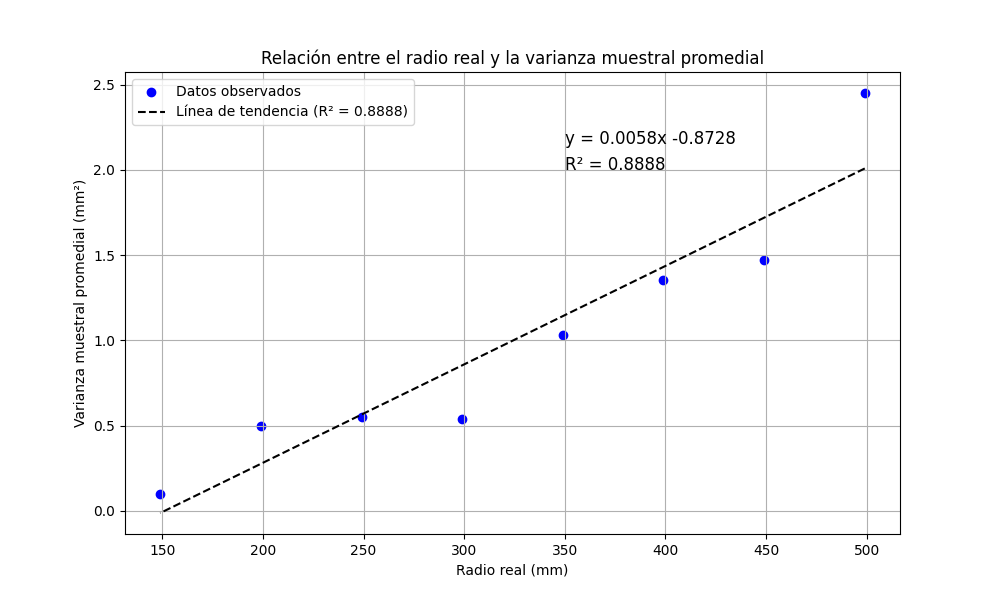
\includegraphics[width=0.95\textwidth]{varianza_tendencia.png}
	\caption{Ajuste lineal para la variación de la varianza en función de la distancia.}
	\label{fig:varianza_tendencia}
\end{figure}

En la Figura \ref{fig:lecturas1}, se aprecia que para el primer círculo, con un radio real de 149 mm, la variabilidad de los puntos medidos fue relativamente baja ($\pm$ 1 mm), con una notable concentración de mediciones cercanas al valor esperado (149 mm). Sin embargo, al aumentar el radio medido, la dispersión de los puntos incrementó hasta $\pm$ 4 mm sobre el valor esperado (499 mm), reflejando una mayor variabilidad en las mediciones (ver Figura \ref{fig:lecturas8}). En cuanto al sesgo o \textit{bias}, la Figura \ref{fig:bias_tendencia} demuestra que no se identificó una tendencia clara, ya que este oscilaba entre aproximadamente -0.9657 mm y 0.9895 mm. Es importante destacar que la varianza muestral, promedio y sesgo reportados en el Cuadro \ref{cuadro:stats} representan los promedios obtenidos en las diez corridas realizadas, proporcionando así una estimación robusta de las mediciones en cada radio. Para una comprensión más detallada de los resultados, en los Anexos \ref{varianza_distancia} se encuentran las estadísticas completas de cada corrida realizada.


\begin{figure}[H]
	\centering
	\makebox[\textwidth]{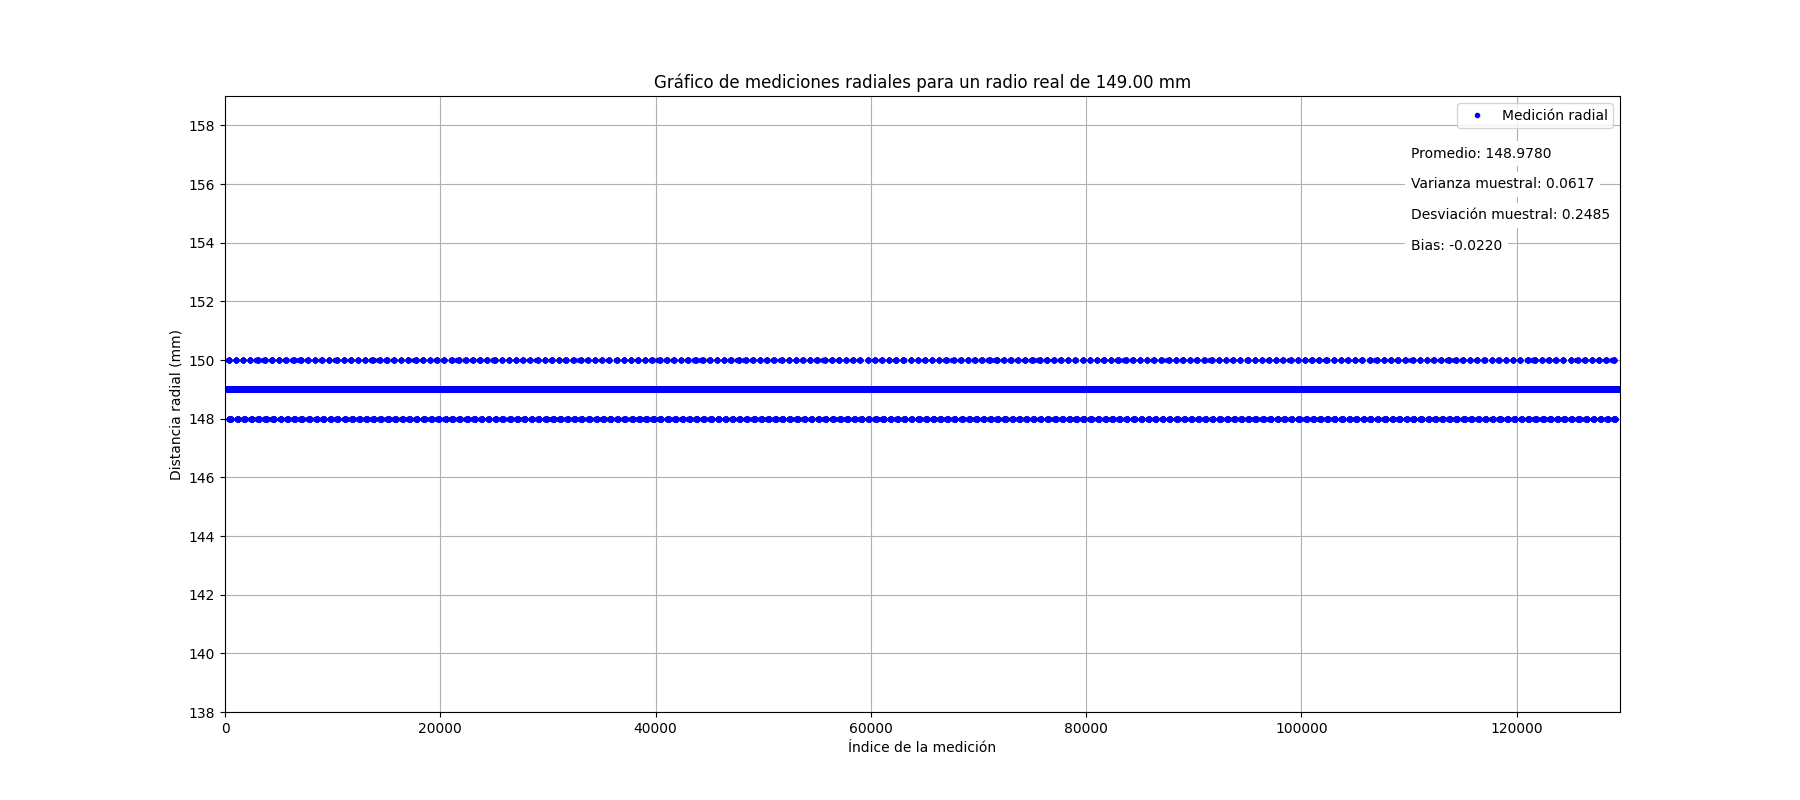
\includegraphics[width=1.25\linewidth]{0.149m_radius_stats_P1.png}}
	\caption{Variabilidad de las mediciones capturadas para un radio real de 149 mm.}
	\label{fig:lecturas1}
\end{figure}

\begin{figure}[H]
	\centering
	\makebox[\textwidth]{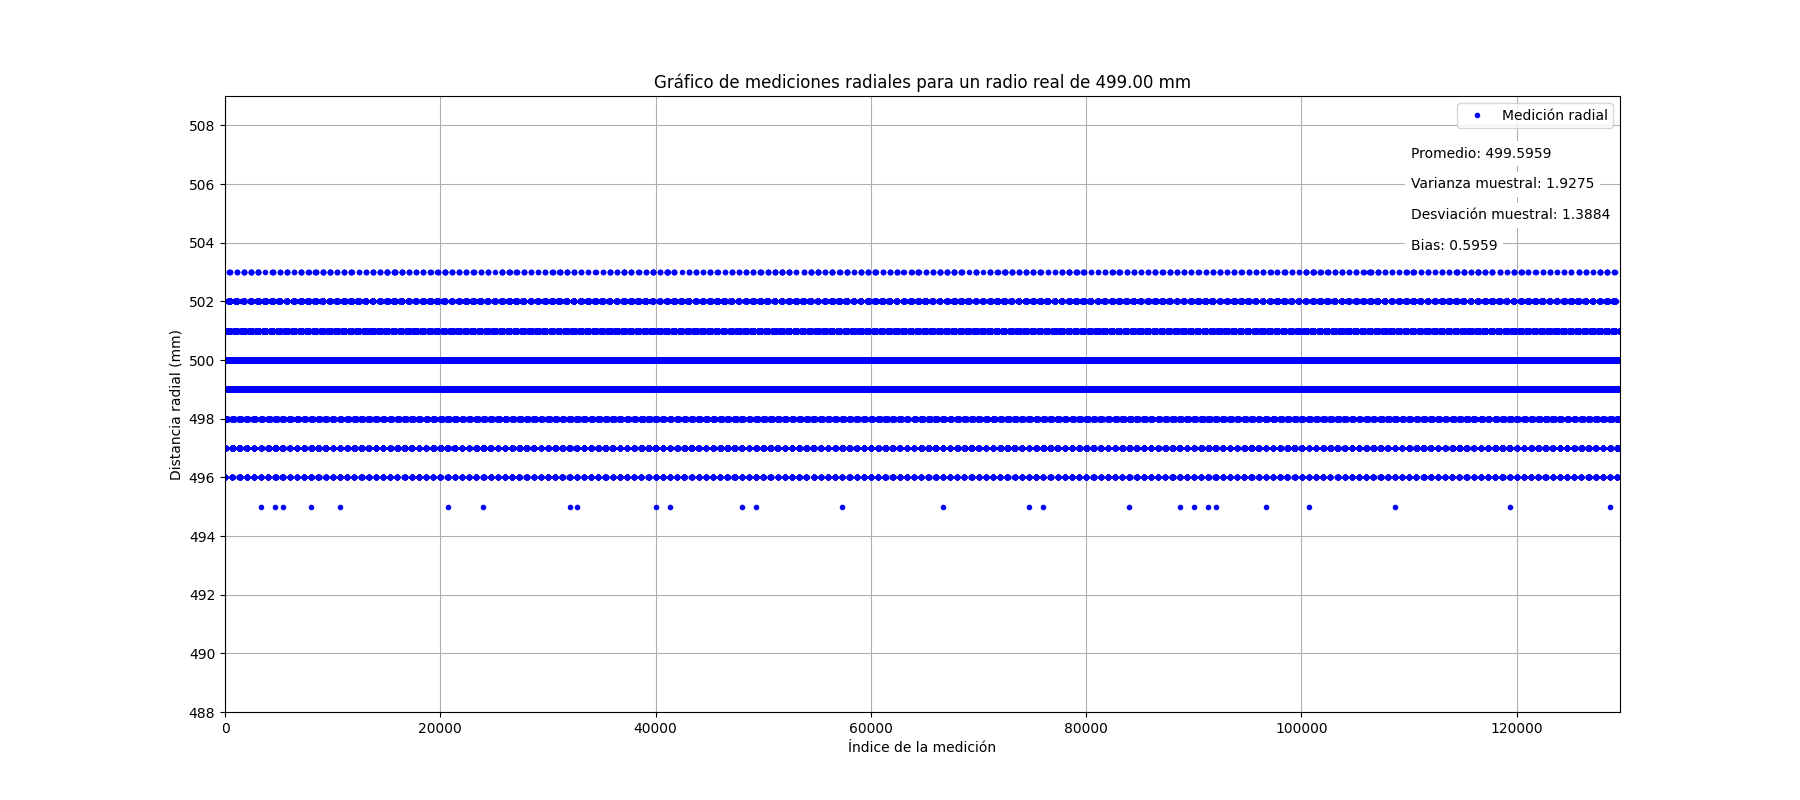
\includegraphics[width=1.25\linewidth]{0.499m_radius_stats_P1.png}}
	\caption{Variabilidad de las mediciones capturadas para un radio real de 499 mm.}
	\label{fig:lecturas8}
\end{figure}

\begin{figure}[H]
	\centering
	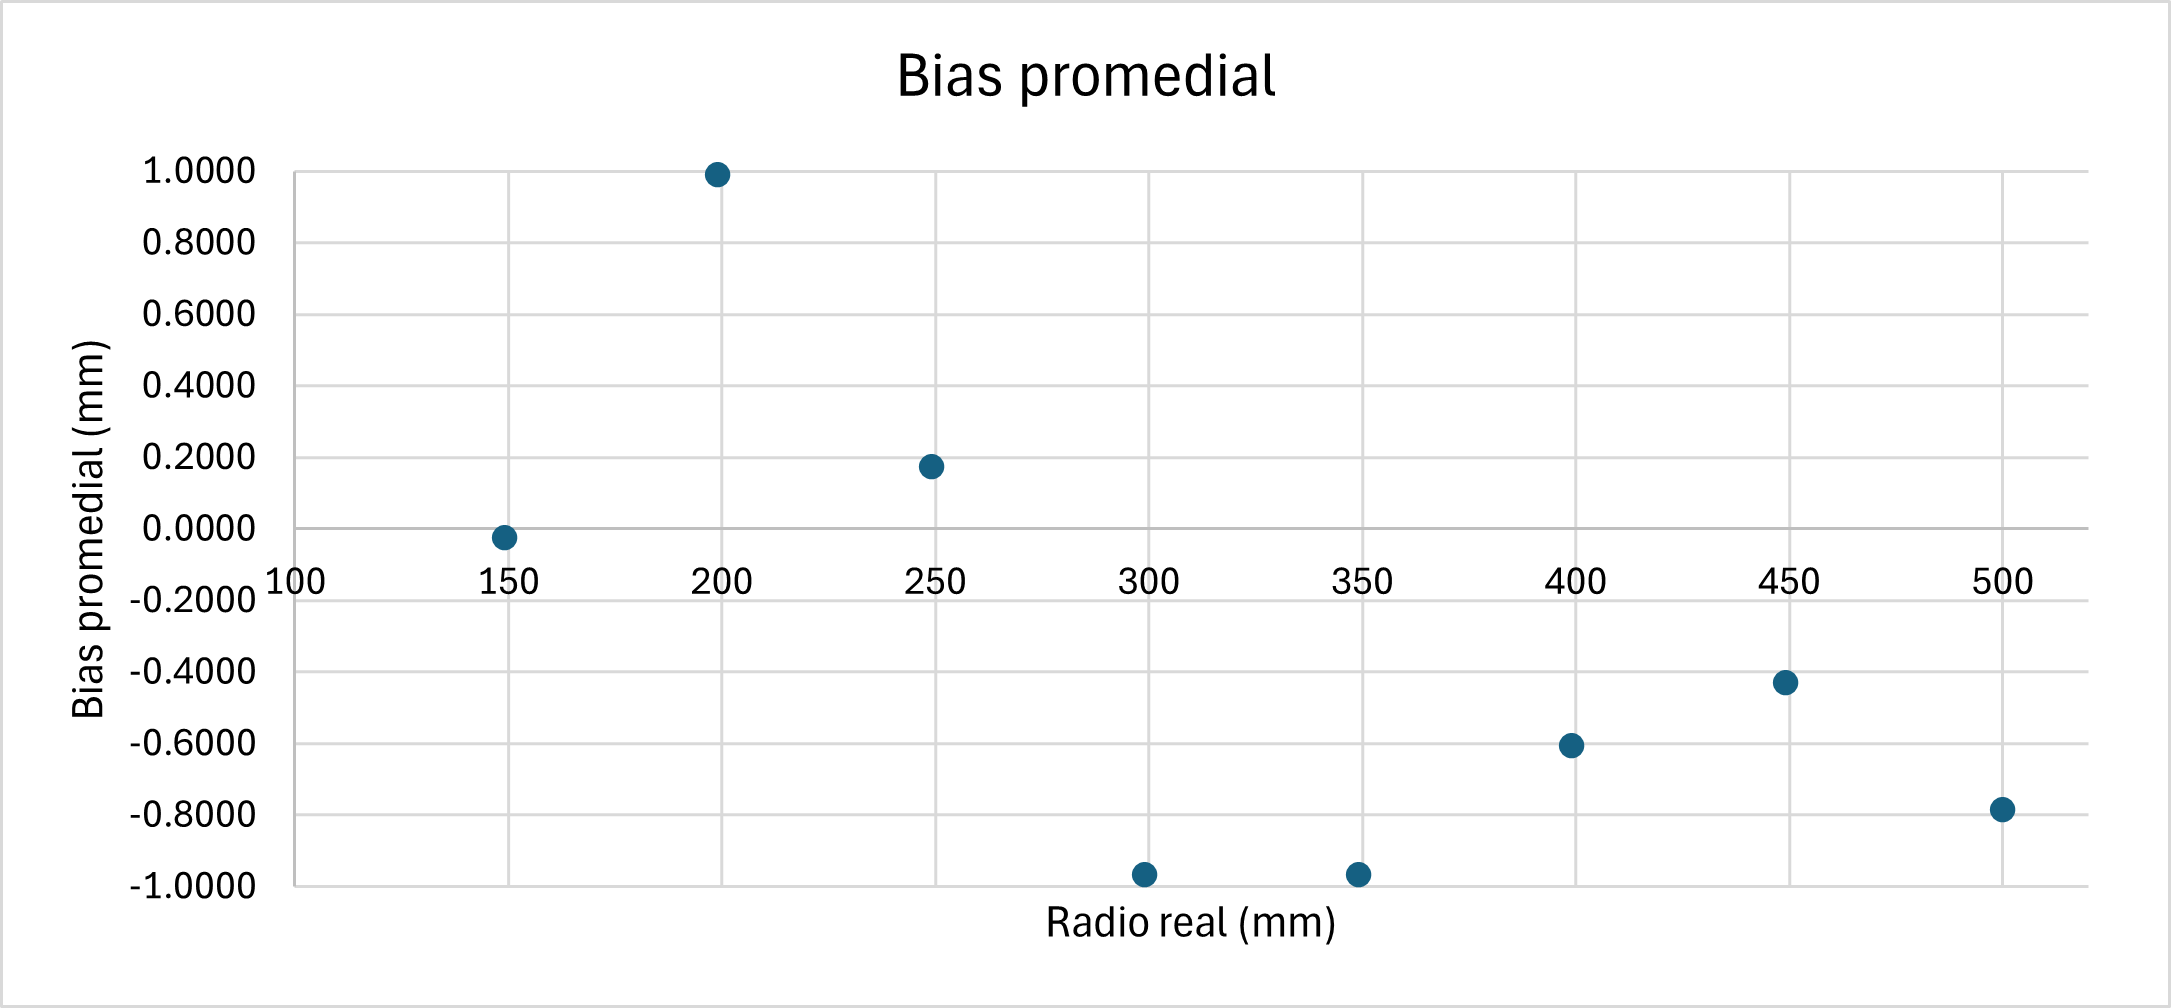
\includegraphics[width=0.8\textwidth]{bias_tendencia.png}
	\caption{Variación del sesgo en función de la distancia.}
	\label{fig:bias_tendencia}
\end{figure}

\subsection{Dispersión de las mediciones angulares del sensor}
\label{mediciones_angulares}
En el segundo experimento, se utilizó el mismo conjunto de círculos del ensayo anterior, añadiendo un noveno círculo de 70 mm de radio, diseñado específicamente para obstruir parcialmente el campo de visión del sensor. Como se muestra en las Figuras \ref{fig:disposicion_lidar_var_theta1} y \ref{fig:disposicion_lidar_var_theta8}, el sensor se mantuvo estático en el centro de la cuadrícula de referencia, mientras se colocaron dos círculos: uno externo, correspondiente a uno de los círculos previamente utilizados, y el círculo de obstrucción visual, con una apertura aproximada de 40° (ver Figura \ref{fig:obstrucción_visual}). Además, se situó un arco circular con un radio 20 mm menor al del círculo externo, abarcando un rango angular de 5°. Esta disposición permitió evaluar cómo las mediciones angulares del sensor respondían a los cambios geométricos entre el círculo y el arco  dentro del área de apertura, enfocando la medición hacia el arco situado frente al círculo externo. Cabe señalar que el arco fue colocado arbitrariamente entre los 42° y 47°, respecto al eje horizontal positivo, definiendo así los puntos de transición teóricos para el análisis.

\begin{figure}[H]
	\centering
	\begin{subfigure}{0.45\textwidth}
		\centering
		\makebox[\textwidth]{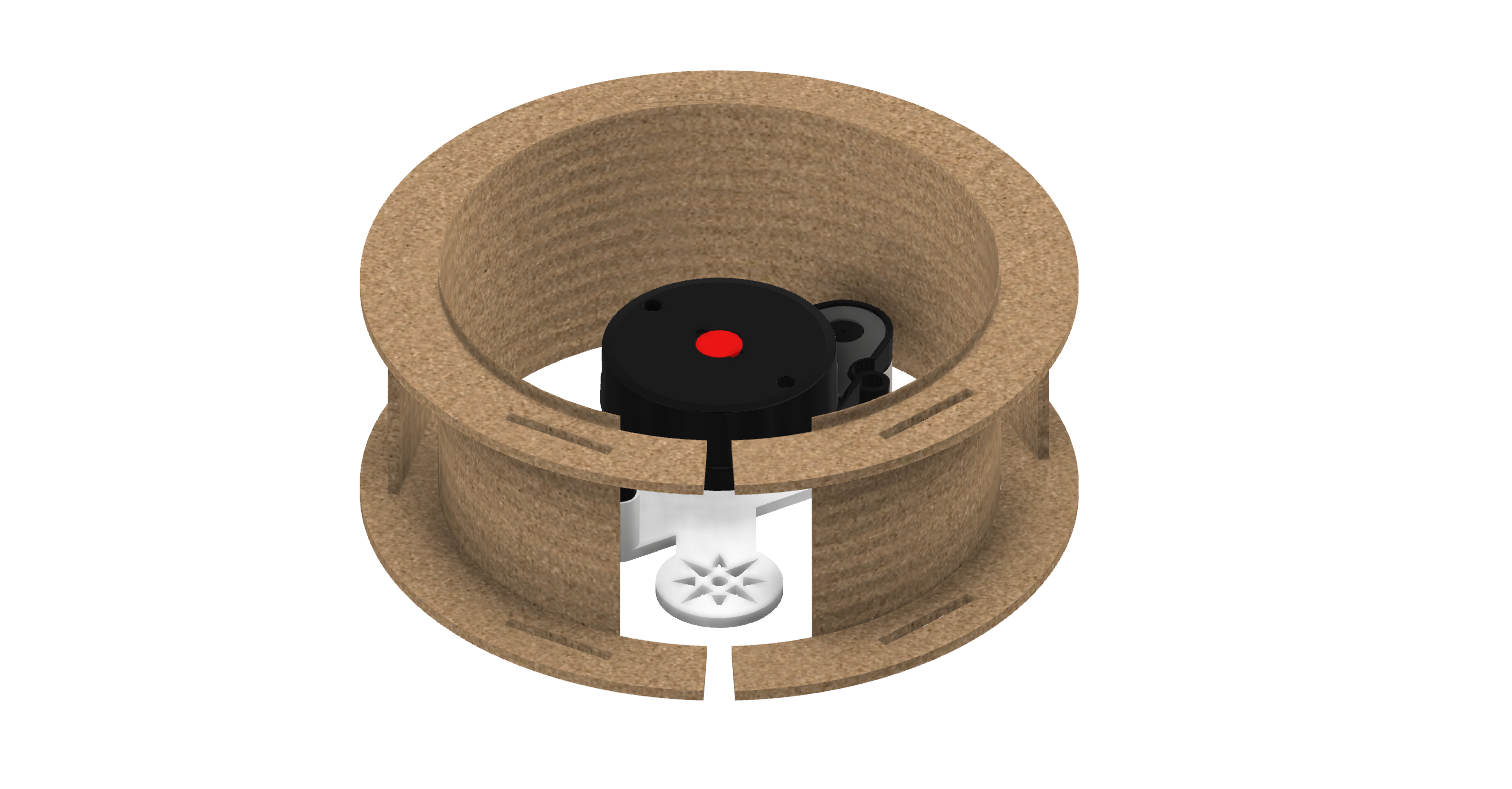
\includegraphics[width=1.15\linewidth]{CIRCULO_OBSTRUCCION_VISUAL.png}}
		\caption{Disposición del sensor FHL-LD20 dentro del círculo de obstrucción visual: 70 mm de radio, vista isométrica frontal.}
		\label{fig:obs1}
	\end{subfigure}
	\hspace{1em}
	\begin{subfigure}{0.45\textwidth}
		\centering
		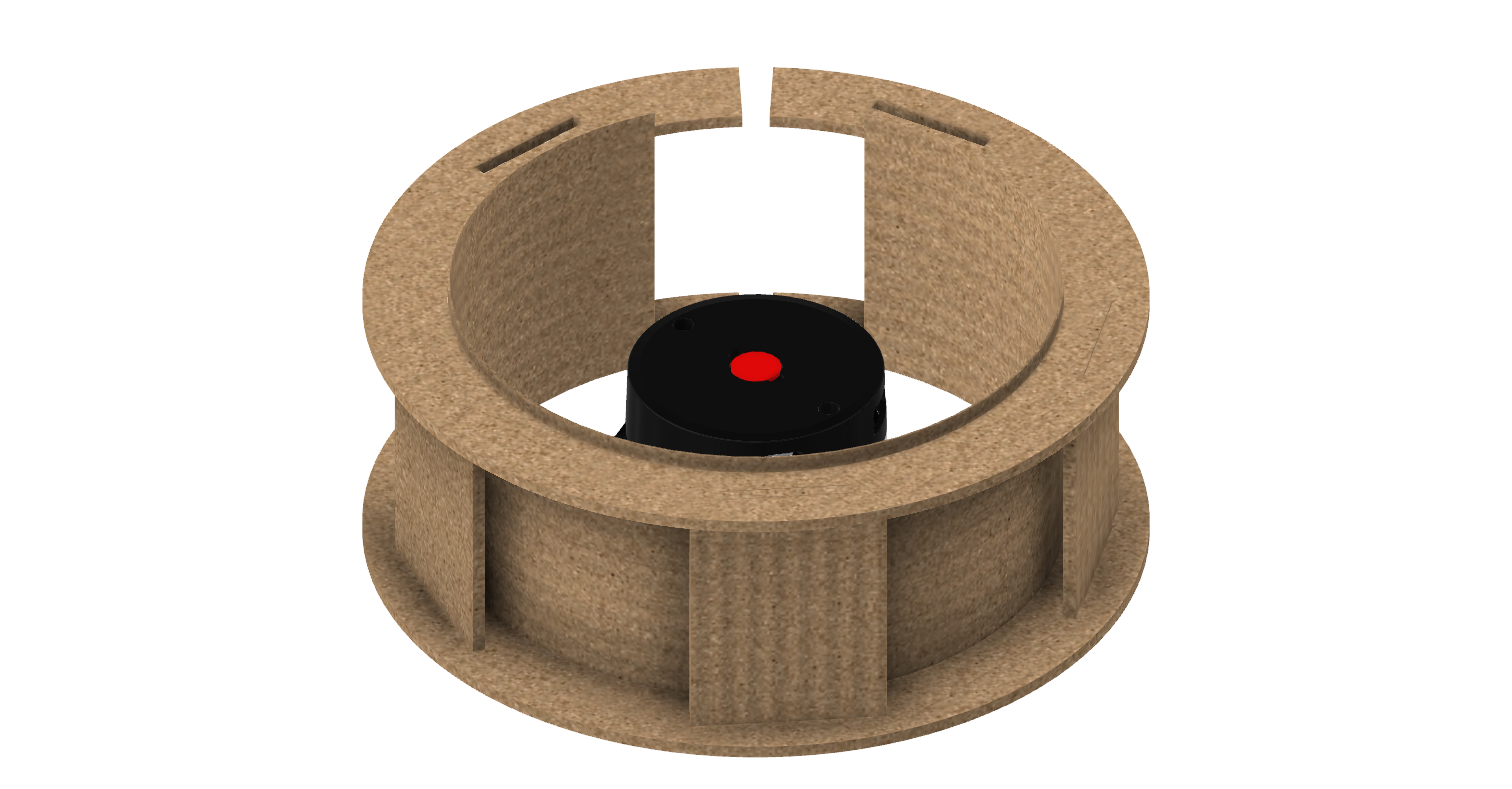
\includegraphics[width=1.15\linewidth]{CIRCULO_OBSTRUCCION_VISUAL_2.png}
		\caption{Disposición del sensor FHL-LD20 dentro del círculo de obstrucción visual: 70 mm de radio, vista isométrica trasera.}
		\label{fig:obs2}
	\end{subfigure}
	\caption{Disposición del sensor FHL-LD20 dentro del círculo de obstrucción visual con apertura de aproximadamente 40°.}
	\label{fig:obstrucción_visual}
\end{figure}

\begin{figure}[H]
	\centering
	\begin{subfigure}{0.45\textwidth}
		\centering
		\makebox[\textwidth]{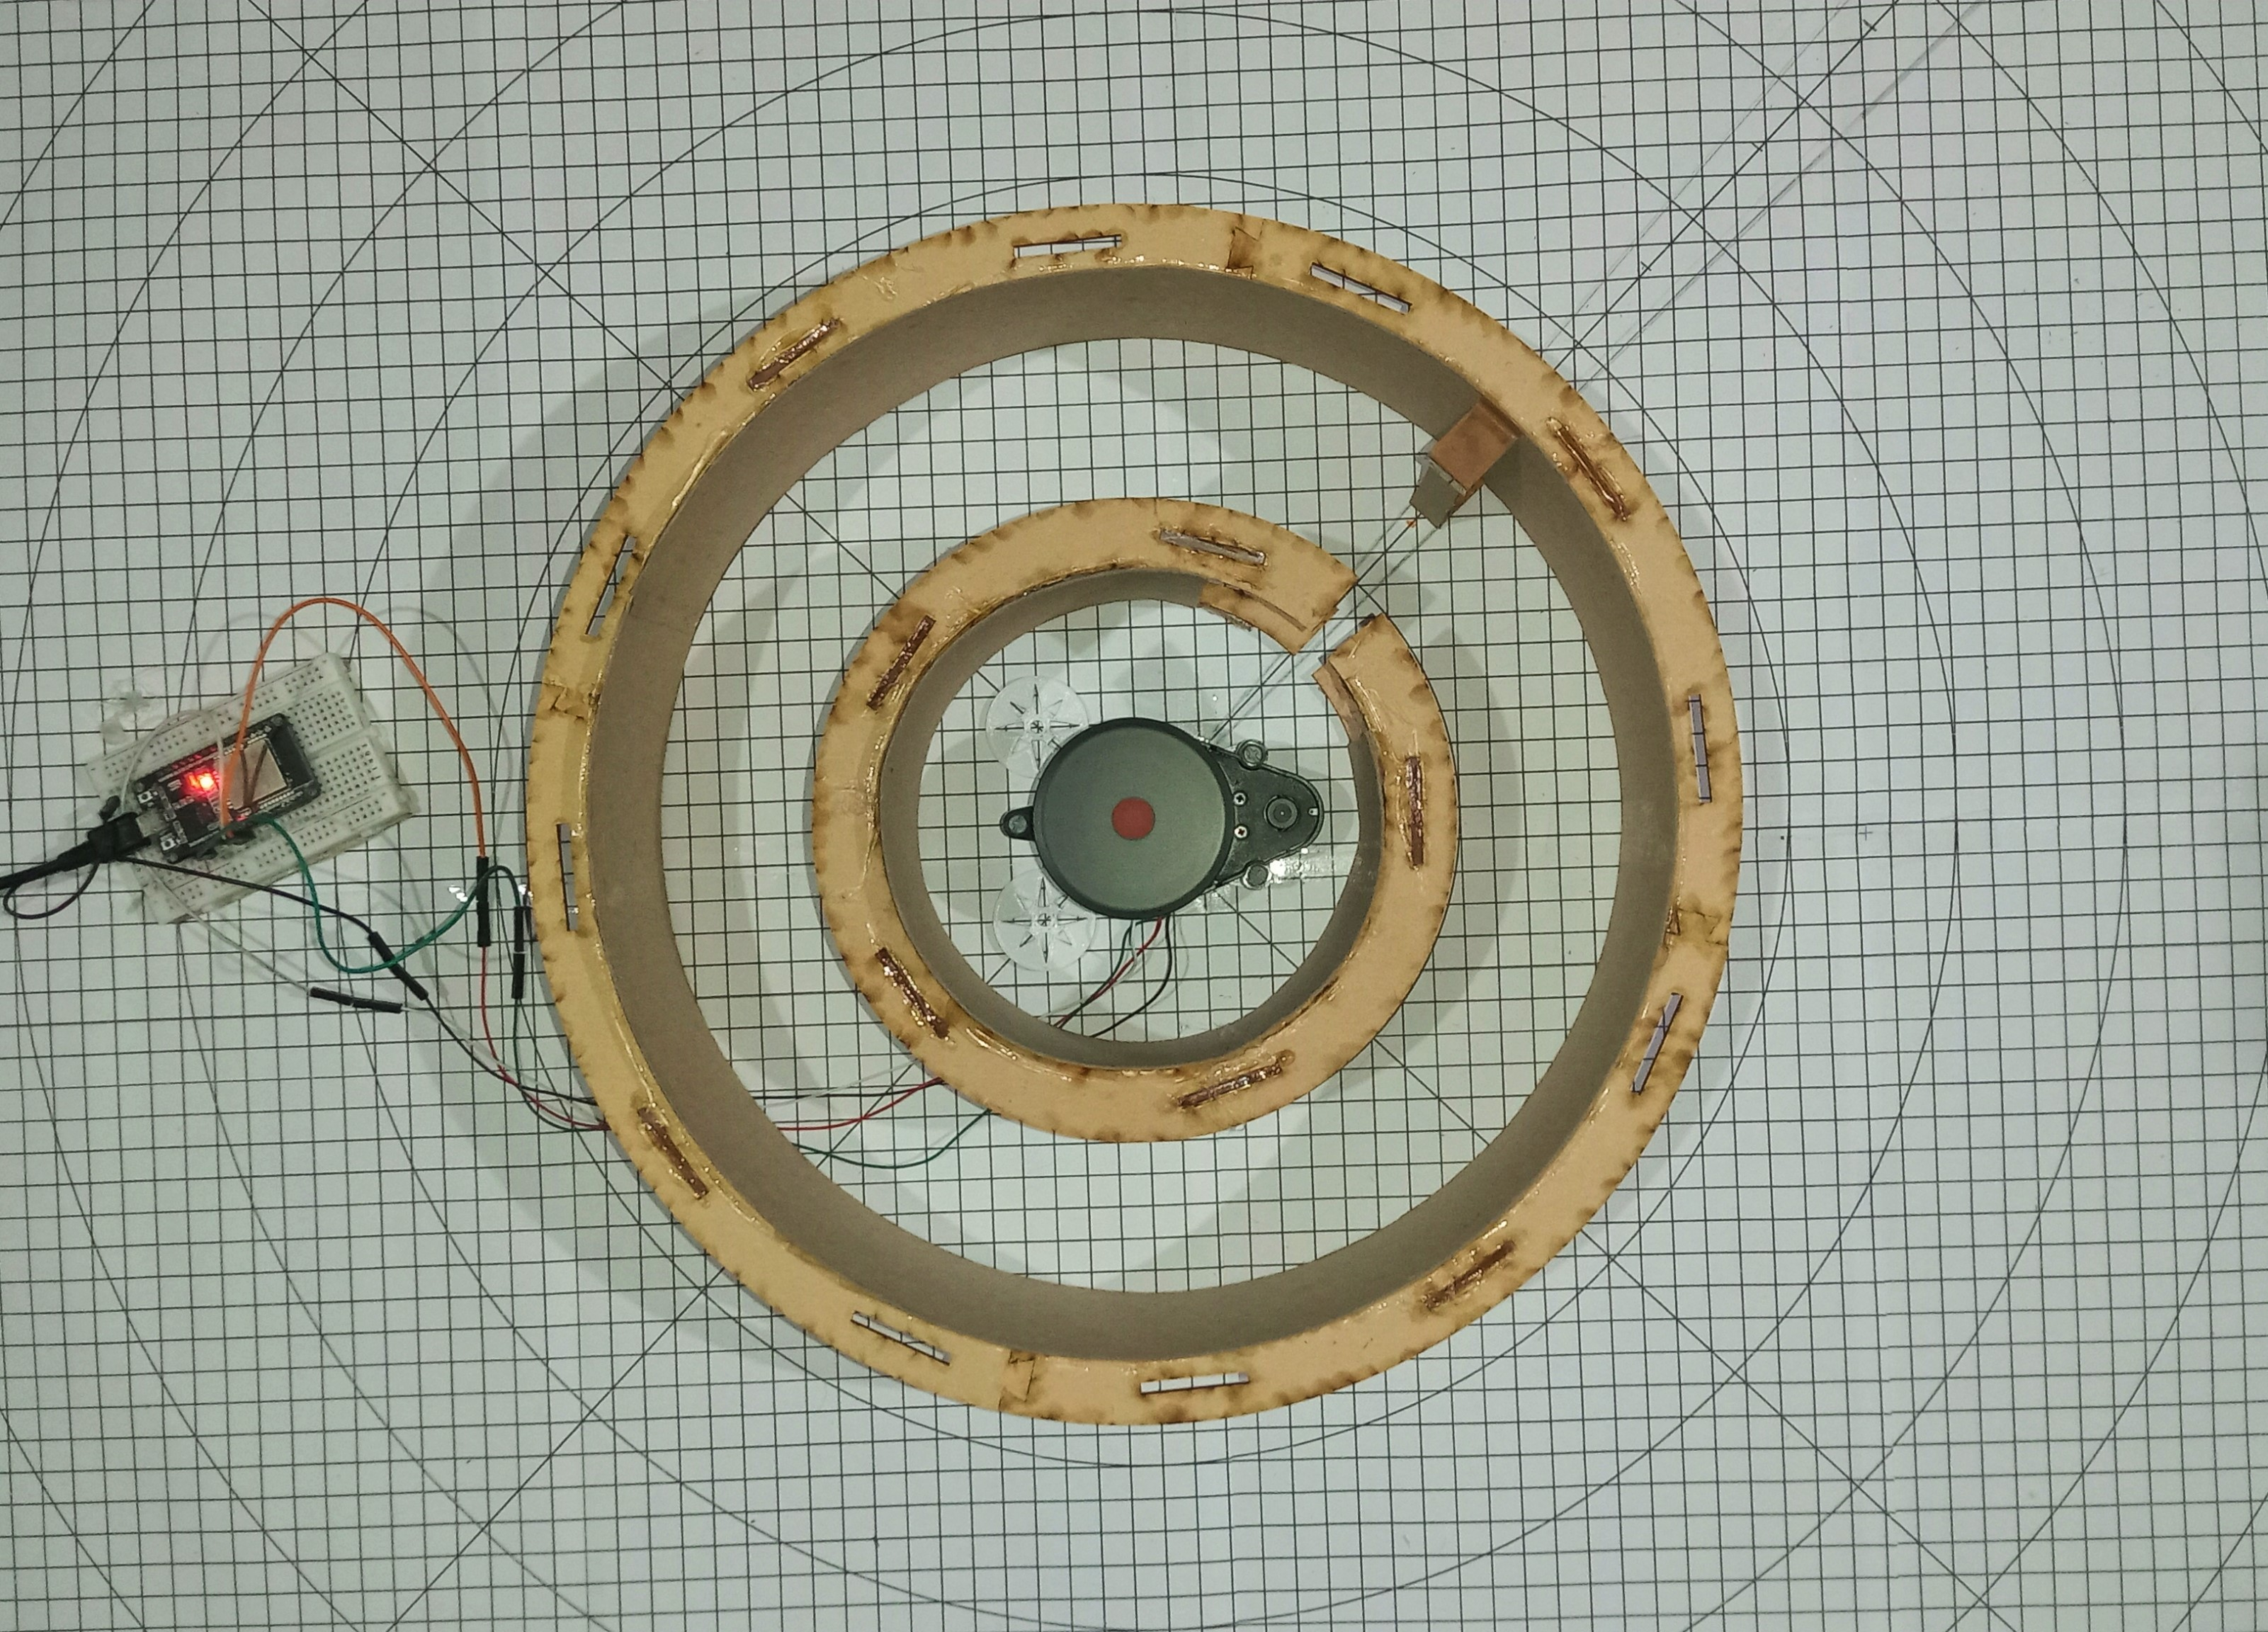
\includegraphics[width=1.15\linewidth]{disposicion_lidar_var_theta1.jpg}}
		\caption{Disposición del sensor FHL-LD20 dentro del entorno circular: 149 mm de radio con arco.}
		\label{fig:disposicion_lidar_theta1}
	\end{subfigure}
	\hspace{1em}
	\begin{subfigure}{0.45\textwidth}
		\centering
		\includegraphics[width=0.85\linewidth]{130mm_theta_XY.png}
		\caption{Reconstrucción en coordenadas cartesianas de entorno circular: 149 mm de radio con arco.}
		\label{fig:149m_radius_xy_theta1}
	\end{subfigure}
	\caption{Reconstrucción del entorno circular de 149 mm de radio con arco, 180 revoluciones completas capturadas.}
	\label{fig:disposicion_lidar_var_theta1}
\end{figure}

\begin{figure}[H]
	\centering
	\begin{subfigure}{0.45\textwidth}
		\centering
		\makebox[\textwidth]{\includegraphics[width=1.15\linewidth]{disposicion_lidar_var_theta8.jpg}}
		\caption{Disposición del sensor FHL-LD20 dentro del entorno circular: 499 mm de radio con arco.}
		\label{fig:disposicion_lidar_theta8}
	\end{subfigure}
	\hspace{1em}
	\begin{subfigure}{0.45\textwidth}
		\centering
		\includegraphics[width=0.85\linewidth]{480mm_theta_XY.png}
		\caption{Reconstrucción en coordenadas cartesianas de entorno circular: 499 mm de radio con arco.}
		\label{fig:499m_radius_xy_theta8}
	\end{subfigure}
	\caption{Reconstrucción del entorno circular de 499 mm de radio con arco, 180 revoluciones completas capturadas.}
	\label{fig:disposicion_lidar_var_theta8}
\end{figure}

Como se observa en la Figura \ref{fig:points}, para evaluar el comportamiento del sensor en estas transiciones, se tomaron cuatro puntos de referencia principales: 
\begin{enumerate}
	\item  La última medición registrada del círculo externo antes de iniciar el arco. 
	\item La primera medición correspondiente al inicio del arco.
	\item La última medición antes de finalizar el arco.
	\item La primera medición del círculo externo tras concluir el arco.
\end{enumerate}
Estos puntos representaron instantes determinantes en las transiciones geométricas, sirviendo como base para analizar la dispersión de las mediciones angulares.

\begin{figure}[H]
	\centering
	\begin{subfigure}{0.8\textwidth}
		\centering
		\includegraphics[width=0.55\linewidth]{480mm_theta_XY_point1.png}
		\caption{El óvalo rojo muestra la ubicación de dos puntos de referencia y su número de identificación.}
		\label{fig:point1}
		\vspace{1em}
	\end{subfigure}
	\begin{subfigure}{0.8\textwidth}
		\centering
		\includegraphics[width=0.55\linewidth]{480mm_theta_XY_point2.png}
		\caption{El óvalo rojo muestra la ubicación de dos puntos de referencia y su número de identificación.}
		\label{fig:point2}
	\end{subfigure}
	\caption{Cuatro puntos de referencia principales en las transiciones de geometría.}
	\label{fig:points}
\end{figure}


Los resultados del experimento se presentan en los Cuadros \ref{cuadro:stats_theta} y \ref{cuadro:stats_theta_r} en Anexos \ref{dispersion_angular}, donde se detallan los rangos de los valores experimentales en los puntos de transición (42° y 47°, respectivamente), para cada uno de los ocho escenarios evaluados, tras capturar 1080 mediciones por ángulo. Al analizar la distribución de estos datos, se determinó que las mediciones angulares seguían una distribución normal (ver Anexos \ref{disposicion_lidar2}), lo que hace que la varianza tradicional no sea la métrica más adecuada para representar la dispersión observada. Por ello, en las Figuras \ref{fig:varianza_circ_47} a \ref{fig:varianza_circ_42} se presentan únicamente los valores mínimo, máximo y promedio de las mediciones angulares en los puntos de referencia. Adicionalmente, en los Figuras \ref{fig:lecturas_theta42_1}) a \ref{fig:histograma_theta47_8} en Anexos \ref{dispersion_angular} se incluyen gráficos que muestran las desviaciones angulares respecto a los valores esperados (deltas de variación) para cada transición.

\begin{figure}[H]
	\centering
	\includegraphics[width=0.95\textwidth]{variacion_circ_arc_47.png}
	\caption{Dispersión angular en la última medición del círculo externo antes del arco a diferentes distancias radiales.}
	\label{fig:varianza_circ_47}
\end{figure}

\begin{figure}[H]
	\centering
	\includegraphics[width=0.95\textwidth]{variacion_arc_47.png}
	\caption{Dispersión angular en la primera medición correspondiente al inicio del arco a diferentes distancias radiales.}
	\label{fig:varianza_arc_47}
\end{figure}

\begin{figure}[H]
	\centering
	\includegraphics[width=0.95\textwidth]{variacion_arc_42.png}
	\caption{Dispersión angular en la última medición justo antes de finalizar el arco a diferentes distancias radiales.}
	\label{fig:varianza_arc_42}
\end{figure}

\begin{figure}[H]
	\centering
	\includegraphics[width=0.95\textwidth]{variacion_circ_arc_42.png}
	\caption{Dispersión angular en la primera medición del círculo externo tras concluir el arco. a diferentes distancias radiales.}
	\label{fig:varianza_circ_42}
\end{figure}

Al analizar los cuatro puntos de referencia, se identificó una mayor dispersión en la última medición del círculo externo antes de iniciar el arco a 47°, y en la última medición del arco antes de regresar al círculo a 42° (ver Figura \ref{fig:point1}). En estos puntos, las mediciones presentaron oscilaciones de entre 0.6210° a 2.8817° respecto a sus valores teóricos. En contraste, el primer punto del arco a 47° y la primera medición del círculo externo tras finalizar el arco a 42° (ver Figura \ref{fig:point2}) mostraron una dispersión considerablemente menor, con fluctuaciones que variaron entre -0.6610° a 0.7625° respecto a los valores teóricos esperados (ver Cuadro \ref{cuadro:dispersion_global}).

\begin{table}[H]
	\centering
	\resizebox{\textwidth}{!}{%
		\begin{tabular}{|c|c|c|c|c|c|c|c|}
			\hline
			\textbf{\makecell{Ubicación de la\\medición obtenida}} & \textbf{\makecell{Valor\\teórico (°)}} & \textbf{\makecell{Mínimo\\local (°)}} & \textbf{\makecell{Diferencia\\con valor\\teórico (°)}} & \textbf{\makecell{Máximo\\local (°)}} & \textbf{\makecell{Diferencia\\ con valor\\ teórico (°)}} & \textbf{\makecell{Mínima\\diferencia\\global\\con valores\\teóricos (°)}} & \textbf{\makecell{Máxima\\diferencia\\global\\con valores\\teóricos (°)}} \\ \hline
			\makecell{Última medición\\registrada del\\círculo externo \\antes de iniciar\\ el arco} & 47 & 47.8190 & 0.8190 & 49.8817 & 2.8817 & \multirow{2}{*}{0.6210} & \multirow{2}{*}{2.8817} \\ \cline{1-6}
			\makecell{Última medición\\antes de \\finalizar el arco.} & 42 & 42.6210 & 0.6210 & 43.8413 & 1.8413 & & \\ \hline
			\makecell{Primera medición\\ correspondiente al \\inicio del arco} & 47 & 46.7588 & -0.2412 & 47.7625 & 0.7625 & \multirow{2}{*}{-0.6610} & \multirow{2}{*}{0.7625} \\ \cline{1-6}
			\makecell{Primera medición\\del círculo externo\\ tras concluir el arco.} & 42 & 41.3390 & -0.6610 & 42.7551 & 0.7551 & & \\ \hline
		\end{tabular}%
	}
	\caption{Resumen de extremos locales y globales respecto al valor teórico.}
	\label{cuadro:dispersion_global}
\end{table}


Para verificar este comportamiento, se repitió el experimento variando la posición del arco, ubicándolo a 222° con respecto al eje horizontal positivo. Al igual que el caso anterior, los resultados mostraron una mayor dispersión en la última medición del círculo externo antes del inicio del arco a 227°, así como en la última medición registrada del arco antes de regresar al círculo externo en 222° (ver Figura \ref{fig:point3}). Estas mediciones oscilaron entre 0.5004° y 2.3290° respecto a los valores teóricos. Por el contrario, las mediciones correspondientes al primer punto del arco a 227° y al primer punto del círculo externo tras finalizar el arco a 222°  (ver Figura \ref{fig:point4}) presentaron una dispersión significativamente menor, con variaciones que se encontraron entre -0.9577° y 0.5750° en relación con los valores teóricos esperados (ver Cuadro \ref{cuadro:dispersion_global_2}). En las Figuras \ref{fig:varianza_circ_227} a \ref{fig:varianza_circ_222} se presentan únicamente los valores mínimo, máximo y promedio de las mediciones angulares en los puntos de referencia.

\begin{figure}[H]
	\centering
	\begin{subfigure}{0.8\textwidth}
		\centering
		\includegraphics[width=0.55\linewidth]{480mm_theta_XY_point4.png}
		\caption{El óvalo rojo muestra la ubicación de dos puntos de referencia y su número de identificación.}
		\label{fig:point3}
		\vspace{1em}
	\end{subfigure}
	\begin{subfigure}{0.8\textwidth}
		\centering
		\includegraphics[width=0.55\linewidth]{480mm_theta_XY_point3.png}
		\caption{El óvalo rojo muestra la ubicación de dos puntos de referencia y su número de identificación.}
		\label{fig:point4}
	\end{subfigure}
	\caption{Cuatro puntos de referencia principales en las transiciones de geometría.}
	\label{fig:points2}
\end{figure}

\begin{figure}[H]
	\centering
	\includegraphics[width=0.95\textwidth]{variacion_circ_arc_227.png}
	\caption{Dispersión angular en la última medición del círculo externo antes del arco a diferentes distancias radiales.}
	\label{fig:varianza_circ_227}
\end{figure}

\begin{figure}[H]
	\centering
	\includegraphics[width=0.95\textwidth]{variacion_arc_227.png}
	\caption{Dispersión angular en la primera medición correspondiente al inicio del arco a diferentes distancias radiales.}
	\label{fig:varianza_arc_227}
\end{figure}

\begin{figure}[H]
	\centering
	\includegraphics[width=0.95\textwidth]{variacion_arc_222.png}
	\caption{Dispersión angular en la última medición justo antes de finalizar el arco a diferentes distancias radiales.}
	\label{fig:varianza_arc_222}
\end{figure}

\begin{figure}[H]
	\centering
	\includegraphics[width=0.95\textwidth]{variacion_circ_arc_222.png}
	\caption{Dispersión angular en la primera medición del círculo externo tras concluir el arco. a diferentes distancias radiales.}
	\label{fig:varianza_circ_222}
\end{figure}

\begin{table}[H]
	\centering
	\resizebox{\textwidth}{!}{%
		\begin{tabular}{|c|c|c|c|c|c|c|c|}
			\hline
			\textbf{\makecell{Ubicación de la\\medición obtenida}} & \textbf{\makecell{Valor\\teórico (°)}} & \textbf{\makecell{Mínimo\\local (°)}} & \textbf{\makecell{Diferencia\\con valor\\teórico (°)}} & \textbf{\makecell{Máximo\\local (°)}} & \textbf{\makecell{Diferencia\\ con valor\\ teórico (°)}} & \textbf{\makecell{Mínima\\diferencia\\global\\con valores\\teóricos (°)}} & \textbf{\makecell{Máxima\\diferencia\\global\\con valores\\teóricos (°)}} \\ \hline
			\makecell{Última medición\\registrada del\\círculo externo \\antes de iniciar\\ el arco} & 227 & 227.5307 & 0.5307 & 229.3290 & 2.3290 & \multirow{2}{*}{0.5004} & \multirow{2}{*}{2.3290} \\ \cline{1-6}
			\makecell{Última medición\\antes de \\finalizar el arco.} & 222 & 222.5004 & 0.5004 & 223.1877 & 1.1877 & & \\ \hline
			\makecell{Primera medición\\ correspondiente al \\inicio del arco}  & 227 & 226.7304 & -0.2696 & 227.5750 & 0.5750 & \multirow{2}{*}{-0.9577} & \multirow{2}{*}{0.5750} \\ \cline{1-6}
			\makecell{Primera medición\\del círculo externo\\ tras concluir el arco.} & 222 & 221.0423 & -0.9577 & 222.5588 & 0.5588 & & \\ \hline
		\end{tabular}%
	}
	\caption{Resumen de extremos locales y globales respecto al valor teórico para ángulos a 222° y 227°, respecto del eje horizontal positivo.}
	\label{cuadro:dispersion_global_2}
\end{table}

Al analizar las reconstrucciones de cada caso en los cuatro puntos de referencia, se observó la presencia de ciertas ``colas'' en las mediciones durante las transiciones de geometría, afectando principalmente las últimas lecturas previas al cambio geométrico. Estas señales residuales, conocidas técnicamente como reflexiones difusas de bordes \cite{diffuse}, se originan por la interacción del LiDAR con transiciones abruptas, donde los bordes de las superficies generan reflexiones parciales del haz infrarrojo, dando lugar a múltiples ecos al recibir la señal. Este fenómeno incrementó la dispersión en las transiciones geométricas, especialmente en las mediciones finales antes del cambio geométrico. 

Estas ``colas'' en la reconstrucción del entrono representan el resultado de un procesamiento incompleto por parte del sensor. Además, la consistencia de este fenómeno en las mediciones confirma que no se trata de un error aleatorio, sino de un comportamiento sistemático inherente de la interacción del sensor con los cambios geométricos. Para reducir estos efectos, se recomienda emplear técnicas de posprocesamiento, como el suavizado de datos o la compensación geométrica mediante algoritmos avanzados de reconstrucción basados en geometrías primitivas \cite{primitive}.

\chapter{Evaluación conceptual para la futura integración del LiDAR FHL-LD20 en agentes robóticos}
En este capítulo se presentan modelos 3D que ilustran posibles montajes del sensor FHL-LD20 en los robots de tracción diferencial Pololu 3pi+. Estos montajes son propuestas conceptuales que exploran cómo podría integrarse el sensor, considerando aspectos como tamaño, espacio disponible, operatividad y limitaciones inherentes a cada configuración. Cada diseño ofrece ventajas y desventajas específicas para su aplicación en tareas de navegación autónoma y mapeo de entornos. Los modelos se han desarrollado respetando las dimensiones, la forma y las características físicas tanto del sensor como del robot, para proporcionar una visión realista de su posible implementación.

\section{Montaje frontal del sensor FHL-LD20}